\documentclass[titlepage,12pt,a4paper,twoside,openright,svgname]{report}%
\addtolength\oddsidemargin {10cm}\addtolength\evensidemargin {-10cm}


% ********************************************************************
% Re-usable information
% ********************************************************************
\newcommand{\myTitle}{Limitador de sonido para locales de música\xspace}
\newcommand{\myDegree}{Grado en Ingeniería Informática\xspace}
\newcommand{\myName}{Alejandro Ruiz Becerra\xspace}
\newcommand{\myProf}{Andrés María Roldán Aranda\xspace}
 \newcommand{\myMateLuis}{Luis Peinado Córdoba\xspace}
 \newcommand{\myMateDani}{Dani Ruiz Medina\xspace}
\newcommand{\myFaculty}{Escuela Técnica Superior de Ingenierías Informática y de
    Telecomunicación\xspace}
\newcommand{\myFacultyShort}{E.T.S. de Ingenierías Informática y de
    Telecomunicación\xspace}
\newcommand{\myDepartment}{Departamento de Electrónica y Tecnología de Computadores\xspace}
\newcommand{\myUni}{\protect{Universidad de Granada}\xspace}
\newcommand{\myLocation}{Granada\xspace}
\newcommand{\myTime}{\today\xspace}
\newcommand{\myVersion}{Version 0.1\xspace}


%\usepackage{dirtree}
%\usepackage{movie15}
%\usepackage{indentfirst}
%\usepackage{enumitem}
\usepackage{afterpage}
\usepackage{soul}
%\usepackage{siunitx}
\usepackage{xcolor}
%\usepackage{xspace}
%\usepackage{mhchem}
\usepackage{amsmath}
%\usepackage{wrapfig}
%\usepackage{changepage}
%\usepackage{geometry}

\usepackage{tabulary}
\usepackage{tabularx}
\usepackage{booktabs}
\usepackage{caption}

\usepackage{float}
\usepackage{color}
\usepackage{upquote}
\usepackage{listings}
\usepackage[singlespacing]{setspace} % package para controlar
\usepackage{estilos/pfc}
\usepackage{estilos/funciones}
\PassOptionsToPackage{spanish,english}{babel}
\usepackage[spanish, english]{babel}
\usepackage{lscape}
\usepackage{graphicx}
\usepackage{epstopdf}
\usepackage{rotating}
\usepackage{hyperref}
\usepackage[noabbrev]{cleveref}      % reference object types automatically

\usepackage{fixltx2e}
\usepackage{longtable}

\usepackage{listings}
\usepackage{eurosym}
\usepackage{pdfpages}

\usepackage{algorithm}      % http://ctan.org/pkg/algorithms
\usepackage{algpseudocode}  % http://ctan.org/pkg/algorithmicx
\usepackage{multirow}
\usepackage{appendix}
\usepackage{subfig}         % subfiguras

%\usepackage[3D]{movie15}
%\usepackage{media9}

\usepackage{url}
\usepackage{enumerate}
\usepackage{inputenc}
%\usepackage{multimedia}

%\usepackage{glossaries}
%\usepackage[acronym]{glossaries}



%\geometry{bindingoffset=3mm}
\def\videoautorefname{Video}%

\newcommand{\heading}[1]{\multicolumn{1}{c}{#1}}


\definecolor{LightBlue}{rgb}{0.83, 0.92, 0.95}
\definecolor{codegreen}{rgb}{0,0.6,0}
\definecolor{codegray}{rgb}{0.5,0.5,0.5}
\definecolor{codepurple}{rgb}{0.58,0,0.82}
\definecolor{backcolour}{rgb}{0.95,0.95,0.92}

%% ALEX %%
%\def\chapterautorefname{Chapter}%
%\def\figureautorefname{Figure}%
%\def\sectionautorefname{Section}%
%\def\subsectionautorefname{Subsection}%
%\def\tableautorefname{Table}%
%\def\equationautorefname{Equation}%

%para que no se corten parrafos a mitad
%\widowpenalties 1 10000
%\raggedbottom

%Video floats
\newfloat{videoFloat}{thp}{lop}[chapter]
\floatname{videoFloat}{Video}


\definecolor{atomString}{RGB}{221,17,68}
\definecolor{atomComment}{RGB}{153,153,136}
\definecolor{black}{RGB}{0,0,0}
\definecolor{mygreen}{RGB}{28,172,0} % color values Red, Green, Blue
\definecolor{mylilas}{RGB}{170,55,241}


% CSS
\lstdefinelanguage{CSS}{
    keywords={color,background-image:,margin,padding,font,weight,display,position,top,left,right,bottom,list,style,border,size,white,space,min,width, transition:, transform:, transition-property, transition-duration, transition-timing-function},
    sensitive=true,
    morecomment=[l]{//},
    morecomment=[s]{/*}{*/},
    morestring=[b]',
    morestring=[b]",
    alsoletter={:},
    alsodigit={-}
}

% JavaScript
\lstdefinelanguage{JavaScript}{
    morekeywords={typeof, delete,new, true, false, catch, function, return, null, catch, switch, var, if, in, while, do, else, case, break},
    morecomment=[s]{/*}{*/},
    morecomment=[l]//,
    morestring=[b]",
    morestring=[b]'
}

\lstdefinelanguage{HTML5}{
    language=html,
    sensitive=true,
    alsoletter={<>=-},
    morecomment=[s]{<!-}{-->},
    tag=[s],
    otherkeywords={
        % General
        >,
        % Standard tags
        <!DOCTYPE,
        </html, <html, <head, <title, </title, <style, </style, <link, </head, <meta, />,
        % body
        </body, <body,
        % Divs
        </div, <div, </div>,
        % Paragraphs
        </p, <p, </p>,
        % scripts
        </script, <script,
        % More tags...
        <canvas, /canvas>, <svg, <rect, <animateTransform, </rect>, </svg>, <video, <source, <iframe, </iframe>, </video>, <image, </image>, <header, </header, <article, </article
    },
    ndkeywords={
        % General
        =,
        % HTML attributes
        charset=, src=, id=, width=, height=, style=, type=, rel=, href=,
        % SVG attributes
        fill=, attributeName=, begin=, dur=, from=, to=, poster=, controls=, x=, y=, repeatCount=, xlink:href=,
        % properties
        margin:, padding:, background-image:, border:, top:, left:, position:, width:, height:, margin-top:, margin-bottom:, font-size:, line-height:,
        % CSS3 properties
        transform:, -moz-transform:, -webkit-transform:,
        animation:, -webkit-animation:,
        transition:,  transition-duration:, transition-property:, transition-timing-function:,
    }
}

\lstdefinestyle{htmlcssjs} {%
    % General design
    backgroundcolor=\color{white},
    basicstyle={\footnotesize\ttfamily},
    frame=b,
    % line-numbers
    xleftmargin={0.75cm},
    numbers=left,
    stepnumber=1,
    firstnumber=1,
    numberfirstline=true,
    % Code design
    identifierstyle=\color{black},
    keywordstyle=\color{blue}\bfseries,
    ndkeywordstyle=\color{black}\bfseries,
    stringstyle=\color{red}\ttfamily,
    commentstyle=\color{atomComment}\ttfamily,
    % Code
    language=HTML5,
    alsolanguage=JavaScript,
    alsodigit={.:;},
    tabsize=1,
    showtabs=false,
    showspaces=false,
    showstringspaces=false,
    extendedchars=true,
    breaklines=true,
    captionpos=b,                    % sets the caption-position to bottom
    literate=%
    *{0}{{{\color{red}0}}}1
    {1}{{{\color{red}1}}}1
    {2}{{{\color{red}2}}}1
    {3}{{{\color{red}3}}}1
    {4}{{{\color{red}4}}}1
    {5}{{{\color{red}5}}}1
    {6}{{{\color{red}6}}}1
    {7}{{{\color{red}7}}}1
    {8}{{{\color{red}8}}}1
    {9}{{{\color{red}9}}}1,
    % German umlauts
    literate=%
    {Ö}{{\"O}}1
    {Ä}{{\"A}}1
    {Ü}{{\"U}}1
    {ß}{{\ss}}1
    {ü}{{\"u}}1
    {ä}{{\"a}}1
    {ö}{{\"o}}1
}
%
\lstdefinestyle{py} {%
    language=python,
    backgroundcolor=\color{white},
    literate=%
    *{0}{{{\color{red}0}}}1
    {1}{{{\color{red}1}}}1
    {2}{{{\color{red}2}}}1
    {3}{{{\color{red}3}}}1
    {4}{{{\color{red}4}}}1
    {5}{{{\color{red}5}}}1
    {6}{{{\color{red}6}}}1
    {7}{{{\color{red}7}}}1
    {8}{{{\color{red}8}}}1
    {9}{{{\color{red}9}}}1,
    basicstyle=\footnotesize\ttfamily, % Standardschrift
    numbers=left,               % Ort der Zeilennummern
    %numberstyle=\tiny,          % Stil der Zeilennummern
    %stepnumber=2,               % Abstand zwischen den Zeilennummern
    numbersep=5pt,              % Abstand der Nummern zum Text
    tabsize=4,                  % Groesse von Tabs
    extendedchars=true,         %
    breaklines=true,            % Zeilen werden Umgebrochen
    keywordstyle=\color{blue}\bfseries,
    frame=b,
    commentstyle=\color{atomComment}\itshape,
    stringstyle=\color{red}\ttfamily, % Farbe der String
    showspaces=false,           % Leerzeichen anzeigen ?
    showtabs=false,             % Tabs anzeigen ?
    xleftmargin=17pt,
    framexleftmargin=17pt,
    framexrightmargin=5pt,
    framexbottommargin=4pt,
    %backgroundcolor=\color{lightgray},
    showstringspaces=false,      % Leerzeichen in Strings anzeigen ?
}

\hypersetup{
    pdfauthor = {\myName (email (en) ugr (punto) es)},
    pdftitle = {\myTitle},
    pdfsubject = {},
    pdfkeywords = {palabra_clave1, palabra_clave2, palabra_clave3, ...},
    pdfcreator = {LaTeX con el paquete ....},
    pdfproducer = {pdflatex}
    %bookmarks=true,% show bookmarks bar?
    %unicode=true, %allows to use characters of non-Latin based languages in Acrobat’s bookmarks
    bookmarksnumbered=true,
    pdfstartview={FitH},
    %– FitH : Fit whole width of page
    %– FitV : Fit whole height of page
    %– FitB : Fit whole ”Bounding Box” page
    %– FitBH: Fit whole width of ”Bounding Box” of page
    %– FitBV: Fit whole height of ”Bounding Box” of page
    pdfpagemode=UseOutlines,
    colorlinks=true,        % false: boxed links; true: colored links
    linkcolor=blue,         % color of internal links
    citecolor=green,        % color of links to bibliography
    filecolor=black,        % color of file links
    urlcolor=blue          % color of external links.
}

\makeindex %Para hacer el índice alfabético

% Glosario
\usepackage[nonumberlist,sanitize={symbol=false},acronym,toc]{glossaries}
\usepackage{glosario_acronimos}
\makeglossaries

%============ ELADIO GUTIERREZ CARRASCO  =====================
% -*- Demosle unas leccioncillas a LaTeX sobre como colocar figuras -*-
\setcounter{topnumber}{3}     % Max. numero de figs. on top
\setcounter{bottomnumber}{3}  % Max. numero de figs. abajo
\setcounter{totalnumber}{10}   % Max. numero de figs. por pagina
\renewcommand{\topfraction}{1} % Max. fraccion de pagina ocupada por figs.
\renewcommand{\bottomfraction}{1}
\renewcommand{\textfraction}{0}  % Min. fraccion de pagina ocupada por texto
\renewcommand{\floatpagefraction}{0.5} % Max. espacio de pagina solo con figs.
\textfloatsep=0.5mm

%Paragraphs
%\parindent=1cm %: indentation of paragraphs
\parskip=3mm %: gap between paragraphs

%OJOOOOOOOOOOOO MARGENES PARA GUILLOTINAR AL IMPRIMIR, QUITAR PARA VERSIÓN DIGITAL. SOLO HAY QUE PONER EL EVEN EN PRINCIPIO
%\addtolength\evensidemargin{3mm}
\addtolength\oddsidemargin{-1.8mm}
%%%%%%%%%%%%%%% ESTO TB PARA IMPRESIÓN,  FIJA EL TAMAÑO EN A4 +3 MM EN CADA LADO
 %\geometry{
		%papersize={216mm,303mm},
 %}
%%%%%%%%%%%%%%%%%%%%%%%%%%%%%%%%%%%

%\oddsidemargin=10mm

%Floats (tables and figures) Parece que no funciona cuando se usa [H]

\floatsep=1mm %: is the space between adjacent floats that are moved to the top or bottom of the text page.
\textfloatsep=1mm %: is the space between the main text and floats at the top or bottom of the page.
\intextsep=5mm %: space left on top and bottom of an in-text float.
%\dbltextfloatsep is \textfloatsep for 2 column output.
%\dblfloatsep is \floatsep for 2 column output.
\abovecaptionskip=0mm %: space above caption
\belowcaptionskip=-2mm %: space below caption

%Maths
\abovedisplayskip=2mm %: space before maths
\belowdisplayskip=2mm %: space after maths
        %\arraycolsep: gap between columns of an array

%Lists
\topsep=1mm %: space between first item and preceding paragraph.
\partopsep=0mm %: extra space added to \topsep when environment starts a new paragraph.
\itemsep=-1.5mm %-2mm %: space between successive items
%\parskip=0mm % 	Space between paragraphs outside of a list, and part of the space between a non-list paragraph and a list item.
%\topsep 	Extra space added to \parskip before the first and after the last item.
%\parsep=0mm %	Paragraph separation within a single item.
%\itemsep 	Extra inter-item spacing added to \parsep.
\partopsep=0mm % 	This is added to the top and/or bottom of the list if and only if there's a blank line above or below the first or last item. Leave this alone unless blank lines become a problem.

%%% NO HYPENATION %%%
\tolerance=1
\emergencystretch=\maxdimen
\hyphenpenalty=10000
\hbadness=10000
%%% NO HYPENATION %%%

\captionsetup{belowskip=10pt,aboveskip=2pt} %%Caption space between figure and below text
%\hypersetup{linkcolor=black, citecolor=black}        % color of links to bibliograp}

% Asignar nombres de secciones no definidos en Babel Spanish
\setlocalecaption{spanish}{contents}{Tabla de contenidos}
\setlocalecaption{spanish}{listfigure}{Lista de figuras}
\setlocalecaption{spanish}{listtable}{Lista de tablas}
\setlocalecaption{spanish}{chapter}{Capítulo}
\setlocalecaption{spanish}{figure}{Figura}
\setlocalecaption{spanish}{appendix}{Apéndice}
\setlocalecaption{spanish}{bib}{Bibliografía}
\setlocalecaption{spanish}{table}{Tabla}

\AtBeginEnvironment{quote}{\par\singlespacing\small}

\newcommand{\commillas}[1]{``#1''}

\usepackage{framed}
\definecolor{shadecolor}{named}{LightBlue}

\definecolor{delim}{RGB}{20,105,176}
\definecolor{numb}{RGB}{106, 109, 32}
\definecolor{string}{rgb}{0.64,0.08,0.08}

\colorlet{punct}{red!60!black}
\definecolor{background}{HTML}{EEEEEE}
\definecolor{delim}{RGB}{20,105,176}
\colorlet{numb}{magenta!60!black}
\lstdefinelanguage{json}{
    basicstyle=\ttfamily\scriptsize,
    numbers=left,
    numberstyle=\tiny\color{codegray},
    stepnumber=1,
    numbersep=8pt,
    showstringspaces=false,
    breaklines=true,
    frame=lines,
    backgroundcolor=\color{background},
    literate=
     *{0}{{{\color{numb}0}}}{1}
      {1}{{{\color{numb}1}}}{1}
      {2}{{{\color{numb}2}}}{1}
      {3}{{{\color{numb}3}}}{1}
      {4}{{{\color{numb}4}}}{1}
      {5}{{{\color{numb}5}}}{1}
      {6}{{{\color{numb}6}}}{1}
      {7}{{{\color{numb}7}}}{1}
      {8}{{{\color{numb}8}}}{1}
      {9}{{{\color{numb}9}}}{1}
      {:}{{{\color{punct}{:}}}}{1}
      {,}{{{\color{punct}{,}}}}{1}
      {\{}{{{\color{delim}{\{}}}}{1}
      {\}}{{{\color{delim}{\}}}}}{1}
      {[}{{{\color{delim}{[}}}}{1}
      {]}{{{\color{delim}{]}}}}{1},
}

\lstdefinelanguage{conf}
{
    basicstyle=\ttfamily\scriptsize,
    numberstyle=\tiny\color{codegray},
    columns=fullflexible,
    morecomment=[l]{\#},
    commentstyle={\color{codegray}\bfseries},
}

\lstdefinestyle{alex}{
%    backgroundcolor=\color{backcolour},
%    commentstyle=\color{codegreen},
%    keywordstyle=\color{magenta},
    numberstyle=\tiny\color{codegray},
%    stringstyle=\color{codepurple},
    basicstyle=\ttfamily\scriptsize,
%    basicstyle=\ttfamily\footnotesize,
%	breakatwhitespace=false,
%    breaklines=true,
%    captionpos=b,
%    keepspaces=true,
%    numbers=left,
%    numbersep=5pt,
%    showspaces=false,
%    showstringspaces=false,
%    showtabs=false,
    tabsize=2
}

\lstset{style=alex}
\usepackage{multicol}

\newcommand{\footlabel}[2]{%
    \addtocounter{footnote}{1}%
    \footnotetext[\thefootnote]{%
        \addtocounter{footnote}{-1}%
        \refstepcounter{footnote}\label{#1}%
        #2%
    }%
    $^{\ref{#1}}$%
}
\renewcommand{\footref}[1]{%
    $^{\ref{#1}}$%
}
%This is a sentence with a footnote\footlabel{rom}{this is the adapted footnote} in it.
%This second sentence points to the same footnote,\footref{rom} so you don't have
%to write it all over again. As you can see, the macro's work in conjuncture with
%the normal\footnote{this is a normal footnote} footnote.
%Though there is a small discrepancy in how the links are displayed.

\begin{document}

\newcommand\blankpage{%
    \null
    \thispagestyle{empty}%
    \addtocounter{page}{-1}%
    \newpage
}

\renewcommand{\arraystretch}{2}

\selectlanguage{spanish}

% Contador de PDF incluidos a pagina completa
\newcounter{includepdfpage}

% Indice alphanumérico
\pagenumbering{alph}

% Portada

\newlength{\originalVOffset}
\newlength{\originalHOffset}
\setlength{\originalVOffset}{\voffset}
\setlength{\originalHOffset}{\hoffset}

\setlength{\voffset}{0cm}
\setlength{\hoffset}{0cm}

\includepdf[pages=-,link=true,landscape]{./Portada/portada_tfm_pablo.pdf}

\setlength{\voffset}{\originalVOffset}
\setlength{\hoffset}{\originalHOffset}

\addcontentsline*{toc}{chapter}{\numberline{}{}}

\pagenumbering{roman} \setcounter{page}{1}

%--
\thispagestyle{empty}
%\includepdf[pages=-,link=true,landscape,linkname=PortadaPastas]{StarTrackerPortada.pdf}

%\cleardoublepage NO METER
%\thispagestyle{empty} NO METER
%\clearpage{\pagestyle{empty}\cleardoublepage} NO METER
%--
%\newpage

\thispagestyle{empty}
\vspace*{3cm}
%\begin{flushright}
%
%%\textbf{\large ``Design of a multidisciplinary 1U CubeSat Simulation Platform''}
%\vfill
%\parindent=0pt
%\begin{small}
%\begin{flushleft}
%Credits for the cover: \textbf{NASA}.\\
%Printed in Granada, September 2019.
%\\~\\
%All rights reserved.
%\end{flushleft}
%
%\end{small}
%
%\afterpage{\blankpage}
%
%\par\end{flushright}{\large \par}

\newpage


%\thispagestyle{empty}
%\vspace*{3cm}
%\begin{flushright}
%
%%\textbf{\large ``Design of a multidisciplinary 1U CubeSat Simulation Platform''}
%
%\textbf{\large ``Design of a multidisciplinary}\\
%\textbf{\large  1U CubeSat Simulation Platform''}
%
%\afterpage{\blankpage}
%
%\par\end{flushright}{\large \par}
%\clearpage

%\thispagestyle{empty}

\begin{center}
\textbf{\huge \includegraphics[scale=1.45]{FigurasTFM/logo_ugr.pdf}}
\par\end{center}{\huge \par}

\begin{center}
\vspace*{1cm}
\par\end{center}

\begin{center}
\textbf{\large GRADO EN}\\
\textbf{\large INGENIERÍA INFORMÁTICA}
\par\end{center}{\large \par}

\begin{center}
\textbf{\large Trabajo de fin de grado}
\par\end{center}{\large \par}

\begin{center}

\par\end{center}

\begin{center}
\textbf{\emph{\LARGE {}``Limitador de sonido}}\\
\textbf{\emph{\LARGE {} para locales de música''}}

\par\end{center}{\LARGE \par}

\begin{center}
\vspace*{3cm}
\par\end{center}

\begin{center}
{\large CURSO ACADÉMICO: 2020 - 2021}
\par\end{center}{\large \par}

\begin{center}
{\large Alejandro Ruiz Becerra}
\par\end{center}{\large \par}

\newpage
\thispagestyle{empty}

~

\newpage
\thispagestyle{empty}

\begin{center}
\includegraphics[scale=1.45]{FigurasTFM/logo_ugr.pdf}
\par\end{center}

\begin{center}
GRADO EN INGENIERÍA INFORMÁTICA\par\end{center}

\begin{center}
\vspace*{0.1cm}
\par\end{center}

\begin{center}
\textbf{\emph{\LARGE {}``Limitador de sonido}}\\
\textbf{\emph{\LARGE {} para locales de música''}}
\par\end{center}{\Large \par}

\begin{center}
\vspace*{0.3cm}
\par\end{center}

\begin{center}
REALIZADO POR:
\par\end{center}

\begin{center}
\textbf{Alejandro Ruiz Becerra}
\par\end{center}

\begin{center}
DIRIGIDO POR:
\par\end{center}

\begin{center}
\textbf{Andrés María Roldán Aranda}
\par\end{center}

\begin{center}
DEPARTAMENTO:
\par\end{center}

\begin{center}
\textbf{Electrónica y Tecnología de Computadores}
\par\end{center}

\begin{center}
\vfill
\par\end{center}

\vspace*{1.5cm}

\newpage
\thispagestyle{empty}
\noindent
\blankpage

%Begin ----  Para que funcione bien el TOC en PDF
\clearpage
\thispagestyle{empty}
\phantomsection
\addcontentsline{toc}{chapter}{Autorización Lectura}

\noindent D. Andrés María Roldán Aranda, Profesor del departamento
de Electrónica y Tecnología de los Computadores de la Universidad
de Granada, como director del Trabajo Fin de Grado de D. Alejandro Ruiz Becerra,

\vspace*{1cm}

Informa:

\begin{doublespace}
Que el presente trabajo, titulado:
\end{doublespace}

\begin{doublespace}
\begin{center}
\textbf{\emph{\large {}``Limitador de sonido para locales de música''}}
\par\end{center}{\large \par}
\end{doublespace}

\noindent ha sido realizado y redactado por el mencionado alumno bajo
mi dirección, y con esta fecha autorizo a su presentación.

\vspace*{1cm}

\begin{center}
Granada, a 21 de Julio de 2021
\par\end{center}

\bigskip
\bigskip
\begin{center}
\includegraphics[scale=0.2]{FigurasTFM/firmaAndres.png}
\end{center}

\begin{center}
\begin{doublespace}
Fdo. Andrés María Roldán Aranda
\end{doublespace}
\end{center}

\newpage
\thispagestyle{empty}
\noindent

\newpage
\phantomsection
\noindent
\blankpage

\addcontentsline{toc}{chapter}{Autorización Depósito Biblioteca}
\bigskip

\noindent Los abajo firmantes autorizan a que la presente copia de
Trabajo Fin de Grado se ubique en la Biblioteca del Centro y/o
departamento para ser libremente consultada por las personas que lo
deseen.

\vspace*{1cm}

\begin{center}
Granada, a 21 de Julio de 2021
\par\end{center}

\bigskip
\bigskip

\begin{center}
\hspace{0cm}\includegraphics[scale=0.9]{FigurasTFM/firmaJC.png}\hspace{3cm} \includegraphics[scale=0.2]{FigurasTFM/firmaAndres.png}
\end{center}

\begin{doublespace}
\begin{center}
\hspace{0cm}Fdo. Alejandro Ruiz Becerra \hspace{3cm} Fdo. Andrés María Roldán Aranda
\end{center}
\end{doublespace}
~

%Begin ----  Para que funcione bien el TOC en PDF
\clearpage
\phantomsection
\noindent
\thispagestyle{empty}


\addcontentsline{toc}{chapter}{Resumen}
\vspace{-1.48cm}
\begin{center}
%\begin{adjustwidth}{-9pt}{0pt}
    \textbf{\Large Limitador de sonido para locales de música}
%\end{adjustwidth}
\par\end{center}{\Large \par}

\begin{center}
    \textbf{\large Alejandro Ruiz Becerra}
    \par\end{center}{\large \par}

\vspace{0.75cm}


\begin{doublespace}
    \noindent \textbf{PALABRAS CLAVE:}
\end{doublespace}


\begin{singlespace}
    \noindent GranaSAT, Acústica y audio, Ingeniería Acústica, Ingeniería Inversa, Control de ruidos, Ecualización, Electrónica.

%    \glsname{cubesat}, \glsname{altium}, Diseño aeroespacial, \glsname{solid}, \glsname{ground}, \acrshort{EDA}, Electrónica, \acrshort{OBC}, \acrshort{ADCS}, \acrshort{EPS}, \acrshort{OBDH}, Diseño de \acrshort{PCB}, \acrshort{matlab}.

\end{singlespace}

\begin{doublespace}
    \noindent \textbf{RESUMEN:}
\end{doublespace}

\begin{singlespace}

    \noindent El objetivo del presente proyecto es diseñar e implementar el software necesario para la construcción de un limitador de sonido para locales de ocio, de forma que se cumplan las especificaciones legales y ordenanzas exigidas por las instituciones en éste ámbito, siendo beneficiara del presente trabajo la empresa \textbf{Heimdal Sound Control}.

    \noindent El proyecto puede dividirse en tres grandes bloques: ingeniería inversa, diseño e implementación. Durante la primera fase se estudian y analizan limitadores de sonido de la competencia, ya presentes en el mercado; para luego diseñar el sistema en base a los requisitos extraídos del proceso de ingeniería inversa, y finalmente desarrollar y probar el software del producto.

    \noindent Este Trabajo de Fin de Grado se sitúa en el ámbito de un proyecto mayor, ambicioso y de largo recorrido, y se apoya en el trabajo realizado por otros alumnos pertenecientes a diversas competencias. Por tanto, el presente trabajo no debe verse como un todo, sino como un gran engranaje dentro de una máquina mayor, el cuál permite que el conjunto de componentes interaccionen entre ellos.

    \noindent La complejidad y el ámbito multidisciplinar de este Trabajo de Fin de Grado permite cubrir, no sólo algunas de las diferentes especialidades del Grado en Ingeniería Informática, sino también adquirir conocimientos y habilidades transversales o específicos de otros campos de la Ingeniería, como la \textbf{Electrónica} y la \textbf{Acústica}.

    \noindent El resultado de todo lo expuesto culmina con un equipo real de limitación de sonido completo y funcional, que cumple con los requisitos definidos en las etapas iniciales del proyecto, y con el cual se cierra la etapa universitaria de Grado.

%    \noindent El objetivo principal del presente proyecto es desarrollar una Plataforma de Simulación multidisciplinar de \textbf{CubeSats}. Estará compuesta de tres bloques diferenciados, en torno a los cuales pivotará el proyecto: una plataforma de simulación mecánica, un software de gestión de \glsname{ground} y un prototipo de \glsname{cubesat}, que constituirá la base del futuro \textbf{GranaSAT-I}.
%
%    Este Trabajo Fin de Máster se aborda desde una ambiciosa doble perspectiva: por un lado, el desarrollo de una Plataforma de Simulación de amplia utilidad en el ámbito académico, como medio para el acercamiento del alumnado de múltiples titulaciones al mundo aeroespacial y en concreto a los CubeSats, en el contexto de auge actual, fomentado por instituciones como la \textbf{Agencia Espacial Europea }(\acrshort{ESA}); en segundo lugar, en el ámbito de investigación, proveyendo de un medio para la implementación de nuevos algoritmos de comunicación, de control orbital y, en general, para el desarrollo y testeo de tecnologías y técnicas novedosas, de manera previa a su lanzamiento.
%
%    El desarrollo e implementación de este proyecto se lleva a cabo siguiendo metodologías de \textbf{Ingeniería de Sistemas} contrastadas y asentadas en la industria espacial, dotándolo de realismo y acercando al alumno a técnicas profesionales de amplio reconocimiento en el mercado de trabajo. Asimismo, la complejidad y ámbito multidisciplinar de este Trabajo~Fin~de~Máster le permite cubrir, no sólo las diferentes especialidades del Máster~de~Ingeniería~de~\textbf{Telecomunicación}, sino también adquirir conocimientos y habilidades transversales o específicos de otros campos de la Ingeniería, como la \textbf{Mecánica} o la \textbf{Aeroespacial}. Así, además de software especialista de cada uno de los campos mencionados, se han analizado y aplicado técnicas avanzadas de \textbf{mecanizado} (fresado de aluminio mediante control numérico), \textbf{fabricación} (soldadura utilizando técnicas de \textit{reflow}) o \textbf{caracterización} de diferentes dispositivos (baterías de litio, células solares de silicio...), entre otros.
%
%    El resultado de todo lo expuesto culmina con la obtención de un entorno de simulación completo y funcional, que cumple con los requisitos definidos en etapas iniciales, y con el cual se cierra la etapa universitaria de Máster.

\end{singlespace}

\vspace{1.25cm}

\newpage

~

\vspace{-1.15cm}


\begin{otherlanguage}{english}

\begin{center}
%\begin{adjustwidth}{-9pt}{0pt}
\textbf{\Large Sound limiter for music venues}
%\end{adjustwidth}
\par\end{center}{\Large \par}

\begin{center}
\textbf{\large Alejandro Ruiz Becerra}
\par\end{center}{\large \par}

\vspace{0.75cm}
\begin{doublespace}
\noindent \textbf{KEYWORDS:}
\end{doublespace}

\begin{singlespace}

    \noindent GranaSAT, Acoustics and audio, Acoustical engineering, Reverse engineering, Noise control, Equalization, Electronics.

%\noindent \glsname{cubesat}, \glsname{altium}, Aerospace design, \glsname{solid}, \glsname{ground}, \acrshort{EDA}, Electronic, \acrshort{OBC}, \acrshort{ADCS}, \acrshort{EPS}, \acrshort{OBDH}, \acrshort{PCB} Design, \acrshort{matlab}.

\end{singlespace}

\begin{doublespace}
\noindent \textbf{ABSTRACT:}
\end{doublespace}

\begin{singlespace}

%    \noindent The complexity and the mutildisciplinary scope of this Bachelor's Thesis allows to cover, not only some of the different specialties of the Bachelor Degree in Informatics Engineering, but also to adquire knowledge and transversal habilities from other fields of the Engineering, such as \textbf{Electronics} and \textbf{Acoustics}.
%
    \noindent El objetivo del presente proyecto es diseñar e implementar el software necesario para la construcción de un limitador de sonido para locales de ocio, de forma que se cumplan las especificaciones legales y ordenanzas exigidas por las instituciones en éste ámbito, siendo beneficiara del presente trabajo la empresa \textbf{Heimdal Sound Control}.

    \noindent El proyecto puede dividirse en tres grandes bloques: ingeniería inversa, diseño e implementación. Durante la primera fase se estudian y analizan limitadores de sonido de la competencia, ya presentes en el mercado; para luego diseñar el sistema en base a los requisitos extraídos del proceso de ingeniería inversa, y finalmente desarrollar y probar el software del producto.

    \noindent Este Trabajo de Fin de Grado se sitúa en el ámbito de un proyecto mayor, ambicioso y de largo recorrido, y se apoya en el trabajo realizado por otros alumnos pertenecientes a diversas competencias. Por tanto, el presente trabajo no debe verse como un todo, sino como un gran engranaje dentro de una máquina mayor, el cuál permite que el conjunto de componentes interaccionen entre ellos.

    \noindent La complejidad y el ámbito multidisciplinar de este Trabajo de Fin de Grado permite cubrir, no sólo algunas de las diferentes especialidades del Grado en Ingeniería Informática, sino también adquirir conocimientos y habilidades transversales o específicos de otros campos de la Ingeniería, como la \textbf{Electrónica} y la \textbf{Acústica}.

    \noindent El resultado de todo lo expuesto culmina con un equipo real de limitación de sonido completo y funcional, que cumple con los requisitos definidos en las etapas iniciales del proyecto, y con el cual se cierra la etapa universitaria de Grado.


%\noindent The main purpose of this project is developing a multidisciplinary Simulation Platform for \textbf{CubeSats}. It will be composed of three differentiated blocks, around which the project is structured: a mechanical simulation platform, a \glsname{ground} management software and a \glsname{cubesat} prototype that will be the base for the future \textbf{GranaSAT-I}.
%
%This Master's Thesis is addressed from a double perspective: on the one hand, the development of a Simulation Platform of great usefulness in an academic environment, as a way to get students from multiple degrees closer to the aerospace world, and particularly to CubeSats, given its current context of peak, being fostered by institutions such as \textbf{European Space Agency} (\acrshort{ESA}); on the other hand, in a research environment, providing with a mean to implement new communication algorithms, orbit controllers, and generally speaking, for the development and test of new technologies and techniques, before launching.
%
%The development and implementation of this project is performed following methodologies of System Engineering contrasted in the aerospace industry, giving realism and getting the student closer to professional techniques, widely recognized in the job market. Furthermore, the complexity and multidisciplinary scope of this Master's~Thesis allows covering not only the different specialties of the Master~in~\textbf{Telecommunication}~Engineering but also acquiring knowledge and transversal abilities from other fields of the Engineering, such as \textbf{Mechanical} or \textbf{Aerospace}. Besides specific software of each of the mentioned areas, advanced techniques of \textbf{machining} (aluminum milling), \textbf{manufacturing} (solder reflow) or \textbf{characterization} of different devices (lithium batteries, silicon solar cells...) among others, have been analyzed and applied.
%
%The result of the exposed culminates with the obtention of a complete and functional simulation environment, which  complies with the requirements defined in the preliminary stages, and supposes the finalization of the Master.
\end{singlespace}

\newpage
\thispagestyle{empty}
%

\end{otherlanguage}

~

%Begin ----  Para que funcione bien el TOC en PDF
\clearpage
\phantomsection
\thispagestyle{empty}
\addcontentsline{toc}{chapter}{Dedication}

\vspace*{8cm}

\begin{quotation}
\noindent \begin{flushright}
%\textbf{\emph{\Large Dedicado a}}\textbf{\emph{\large }}\\
\textbf{\emph{\large \lq Tough and competent\rq}}\\
%\textbf{\emph{  Eugene F. Kranz}}\\
%\textbf{\emph{\large Answer}}\\
%\textbf{\emph{\large \lq --Whatever it takes\rq}}\\
%\textbf{\emph{\large Mis padres, Paco y Encarni, y mi hermano Alberto, porque sin ellos y sin su apoyo, llegar hasta aquí hubiera sido imposible.}}
%\textbf{\emph{\large .....Esto lo último.....}}
%Todos aquellos que no tuvieron la oportunidad.
\par\end{flushright}{\large \par}
\end{quotation}
\newpage
\thispagestyle{empty}


% Agradecimientos
\phantomsection
\addcontentsline{toc}{chapter}{Agradecimientos}
\newpage

\begin{center}
\noindent
\textbf{\emph{\Large Acknowledgments:}}
\vspace{4cm}
\end{center}

This work is dedicated to all those people: family, friends, colleagues, who have supported me throughout my life, and especially in recent years; as well as to all those professors and teachers, who through the great passion and dedication that they pour into their work have contributed to the fact that today I am writing these lines

\newpage
\afterpage{\blankpage}
\newpage


\begin{center}
\noindent
\textbf{\emph{\Large Agradecimientos:}}
\vspace{4cm}
\end{center}

Este trabajo va dedicado a todas aquellas personas: familiares, amistades, compañeros y compañeras, que me han apoyado a lo largo de mi vida, y especialmente durante estos últimos años; así como a todos aquellos profesores y profesoras, universitarios y no universitarios, que mediante la gran pasión y dedicación que vuelcan en su trabajo han contribuido a que hoy me encuentre redactando estas líneas.

\afterpage{\blankpage}


% Lista de FIGURAS
\include{prefacios/ListaFiguras}

% Lista de Videos
%%Begin ----  Para que funcione bien el TOC en PDF
\cleardoublepage
\phantomsection \label{listofvid}
\addcontentsline{toc}{chapter}{List of Videos}
%END  ---- Para que funcione bien el TOC en PDF
 
\begin{singlespacing}%onehalfspacing}
\listof{videoFloat}{List of Videos}
\end{singlespacing}%onehalfspacing}


%\fancyhead{}
%\fancyhead[RO]{\small{\nouppercase{Índice de Figuras}}}
%\fancyhead[LE]{\small{\nouppercase{Índice de Figuras}}}

%\addcontentsline{toc}{chapter}{Lista de Figuras}%

\clearpage{\pagestyle{fancy}\cleardoublepage}%


% Lista de TABLAS
%Begin ----  Para que funcione bien el TOC en PDF
\cleardoublepage
\phantomsection \label{Tablas}
%\addcontentsline{toc}{chapter}{List of Tables}
%END  ---- Para que funcione bien el TOC en PDF
\begin{singlespacing}%onehalfspacing}
\listoftables
\end{singlespacing}%onehalfspacing}

%
%\fancyhead{}
%\fancyhead[RO]{\small{\nouppercase{Índice de Tablas}}}
%\fancyhead[LE]{\small{\nouppercase{Índice de Tablas}}}

%\addcontentsline{toc}{chapter}{Lista de Tablas}%

\clearpage{\pagestyle{fancy}\cleardoublepage}%




% Glosario
\clearpage
\printglossary[style=long3col, type=\acronymtype, title=Acrónimos, toctitle=Acrónimos]
\clearpage
\printglossary[type=main, title=Glosario, toctitle=Glosario]
\clearpage

% Indice árabe
\pagenumbering{arabic}

% Capítulo 1: Introducción
\chapter{Introducción}\label{cap:capitulo1}

El presente proyecto se desarrolla en el marco del Trabajo de Fin de Grado con el cual se finaliza el Grado Universitario en Ingeniería Informática, con especialidad en Ingeniería del Software, cursado por el alumno Alejandro Ruiz Becerra en la Escuela Técnica Superior de Ingenierías Informática y de Telecomunicación de la Universidad de Granada. El objetivo principal del presente trabajo es demostrar los conocimientos y habilidades adquiridos por el alumno durante la realización de dicho Grado. Para ello, se ha realizado el presente proyecto, el cual propone el diseño e implementación de un software que permita controlar los niveles acústicos en locales con equipos de música.

Este Trabajo de Fin de Grado se realiza en colaboración con el proyecto académico \gls{granasat}, un proyecto multidisciplinario, dirigido por el Profesor Andrés María Roldán Aranda, que reúne a personas de diferentes campos que quieren adquirir conocimientos relativos a la Ingeniería Aeroespacial y a la Ingeniería Electrónica.

% EJEMPLO DE IMAGEN CENTRADA
\begin{figure}[H]
    \centering
    
\includegraphics{figuras/granasat.pdf}
    \caption{Logotipo de \gls{granasat}}
    %\vspace{-1cm}
\end{figure}

El laboratorio de \gls{granasat} así como el equipamiento y materiales necesarios para la realización de este proyecto se encuentran en la Avenida de Madrid, frente al Escuela Internacional de Posgrado de la Universidad de Granada y el Antiguo Hospital Clínico de Granada (España). Este proyecto ha sido desarrollado tanto presencialmente en el laboratorio como de forma remota, debido a la situación actual de pandemia causada por el virus COVID-19.

%Es importante destacar que el proyecto que se expone en este documento se basa y apoya en el trabajo realizado por otros alumnos/as antes que yo, así como en el trabajo conjunto que se ha realizado en el presente curso académico con Dani ----, estudiante del Grado en Ingeniería Informática y Luis ----, estudiante del Máster en Ingeniería en Telecomunicaciones, ambos pertenecientes a la Universidad de Granada.

\section{Motivación}\label{sec:motivacion}

% No mostrar las sub-secciones de esta sección
\addtocontents{toc}{\protect\setcounter{tocdepth}{0}}

Todos los establecimientos comerciales que dispongan de equipos de reproducción musical o audiovisual pueden, especialmente de noche, afectar no solo al descanso de los vecinos, sino también a la salud auditiva de los clientes y a los trabajadores del mismo. Es por ello que surge la necesidad de controlar la emisión de ruidos desde estos establecimientos tanto hacia a las viviendas o oficinas adyacentes, como a la calle, así como mantener unos niveles acústicos adecuados en el interior del local. Esta necesidad se hace requisito para este tipo de establecimientos debido a la Ley del Ruido del año 2003.

La Ley del Ruido (Ley 37/2003) del 17 de noviembre de 2003 dio lugar al comienzo de la lucha legislada contra la contaminación acústica, mediante la cual se dota de un esquema básico a nivel estatal para que, en los niveles autonómico y local puedan elaborarse promulgaciones de esta ley. Por tanto, queda en manos de las comunidades autónomas, y en última instancia, de los ayuntamientos, el definir las medidas, normas e infracciones a aplicar en esta materia.

El Ayuntamiento de Granada aplica su propia normativa en este ámbito mediante la \textit{Ordenanza Municipal de Protección del Medio Ambiente Acústico en Granada} del año 2007. Es de especial interés, dado el proyecto que nos ocupa, los artículos 36 y 37.

\subsection{Artículo 36. Condiciones acústicas particulares en actividades y edificaciones donde se generan niveles elevados de ruido}

En este artículo se definen una serie de condiciones para los establecimientos de espectáculos públicos, actividades recreativas y comerciales que generen elevados niveles de ruido.

A modo de resumen, este artículo:

\begin{itemize}
    \item Clasifica las edificaciones donde se generan un nivel de ruido superior a 70 \gls{dba} en 3 tipos.

    \item Exige la aplicación de un aislamiento acústico al local.

    \item Prohíbe niveles de de presión sonora superiores a 90 \gls{dba} en zonas destinadas al público, salvo que se dé advierta correctamente en los accesos a dichas zonas.
\end{itemize}

%Las edificaciones de Tipo 3 se definen como:
%
%\begin{quote}
% Los establecimientos de espectáculos públicos y actividades recreativas, con actuaciones y conciertos con música en directo, y/o música pregrabada bailable, (salas de fiestas, discotecas y cualquier otro establecimiento de esparcimiento)
%\end{quote}

Si bien, estos tipos de establecimientos tienen la obligación de aislar acústicamente el local mediante la aplicación de diferentes soluciones arquitectónicas, esto no es suficiente para garantizar que no se sobrepasan los límites de emisión e inmisión de ruido definidos en la normativa, la cual se puede consultar en el Anexo B. Esto mismo queda reflejado en el articulo 37 de la normativa que puede verse a continuación.

\subsection{Artículo 37. Instalación de equipos limitadores controladores acústicos}

\begin{quote}
    En aquellos locales descritos en el artículo 36 de la presente Ordenanza, donde se disponga de equipo de reproducción musical o audiovisual en los que los niveles de emisión sonora pudieran de alguna forma ser manipulados directa o indirectamente, se instalará un equipo limitador-controlador que permita asegurar, de forma permanente, que bajo ninguna circunstancia las emisiones del equipo musical superen los límites admisibles de nivel sonoro tanto en el interior del propio local (articulo 20 bis) como en las edificaciones adyacentes, así como que cumplen los niveles de emisión al exterior exigidos en esta Ordenanza.
\end{quote}

Por tanto, resulta evidente observar que existe una necesidad por parte de los establecimientos con equipos de reproducción de música de controlar sus niveles de contaminación acústica de forma que se cumpla la normativa, para evitar molestias a vecinos, y denuncias y sanciones a los propietarios del local.

% Reestablecer profundidad del ToC
\addtocontents{toc}{\protect\setcounter{tocdepth}{5}}

\section{Objetivos del proyecto}\label{sec:objetivos}

El objetivo primario de este proyecto es el siguiente:

\begin{itemize}
    \item Presentar un software capaz de registrar los niveles acústicos de emisión y recepción, y que actúe sobre dichos niveles en base a la normativa aplicada.
\end{itemize}

Este objetivo general define de forma concreta qué es lo que se pretende hacer en el proyecto. Asimismo, existen otros objetivos más específicos:

\begin{enumerate}

    \item Conocer y analizar las necesidades reales del sistema de monitorizacion de ruido ambiental requerido.

    \item Extraer los requisitos funcionales y no funcionales del sistema, a partir de conversaciones con el cliente y del proceso de ingeniería inversa.

    \item Realizar una análisis de las tecnologías utilizadas en el software presente en el limitador del laboratorio, y estudiar si pueden solucionar las necesidades de cada uno de los requisitos.

    \item Diseñar e implementar un prototipo del producto software requerido.

    \item Realizar los tests de validación y pruebas necesarios para verificar el correcto funcionamiento del prototipo.

    \item Acercar al alumno a un entorno real de Ingeniería.

    \item Poner de manifiesto los conocimientos y habilidades adquiridas en el Grado de Ingeniería Informática.

    \item Superar la signatura de Fin de Grado, y por ende, el Grado en Ingeniería Informática.
\end{enumerate}

\section{Contexto} \label{sec:contexto}

Hasta ahora, se han establecido cuales son las necesidades y las motivaciones del proyecto, así como la idea general y los objetivos del mismo, pero nada se sabe aún de su punto de partida ni de su contexto, ¿se va a partir de cero? ¿existe una arquitectura hardware específica para este propósito o es parte del proyecto definirla y construirla? ¿hay más personas involucradas en el proyecto? En las siguientes páginas resolveremos estás cuestiones y más, y se proporcionará un enfoque más detallado y completo del la envergadura del trabajo que en este documento se presenta.

%Una vez establecidas las ideas generales del proyecto, es necesario enmarcarlo en su contexto. Las siguientes páginas tendrán como propósito presentar el punto de partida y el contexto del proyecto, de forma que se pueden entender mejor cuál es el ámbito

Para comenzar, en el laboratorio de \glsname{granasat} se dispone de un limitador de sonido operativo, pero bastante antiguo, el cual es necesario estudiar para poder entender se funcionamiento y, por ende, conocer cuales son las tareas concretas que debe realizar un limitador de sonido para efectuar sus funciones. Este limitador será objeto que un minucioso proceso de ingeniería inversa, del cual extraeremos una gran cantidad de conocimiento, en forma de requisitos, diagramas y estrategias de acción para resolver las problemáticas a las que nos enfrentamos en el proyecto. Se dispone así mismo del todo el código fuente de este limitador, lo cual facilitará bastante nuestro trabajo.

Se dedicará un capítulo completo a este limitador, dónde se detallará el proceso de ingeniería inversa al que se le ha sometido, se explicará cómo funciona este limitador y se expondrán todos los conocimientos que se han podido extraer del él. Este limitador, por tanto, supondrá el punto de partida y la principal guía del presente proyecto, siendo así su piedra angular, ya que se volverá é constantemente para comparar y validar el trabajo realizado.


¡¡ INSERTAR IMAGEN DEL LIMITADOR !!


También en laboratorio de \glsname{granasat} se dispone de un limitador en fase de prototipo, sobre el cual correrá el sistema de limitación y control de sonido que se va a desarrollar. Esta arquitectura supone la inclusión de ciertas restricciones y consideraciones a la hora de diseñar e implementar el sistema, ya que se dispone de un hardware especializado y cuyo centro de cómputo es una Raspberry Pi.


¡¡INSERTAR IMAGEN DEL LIMITADOR NUEVO !!


\myMateLuis, es un estudiante del Máster en Ingeniería de Telecomunicaciones y el responsable de esta arquitectura. El trabajo realizado en este prototipo supone su Trabajo de Fin de Máster.

¡¡INSERTAR IMAGEN DE LUIS !!

Por otro lado, es necesario poder configurar el sistema cuando se realice la instalación del mismo en el establecimiento. Los datos configurables en el equipo supondrán unos requisitos de datos y especificarán en el capítulo \ref{cap:capitulo2}, pero a modo de resumen, es necesario configurar una serie de variables que modificarán el funcionamiento del sistema, como el aislamiento aplicado al local y la normativa del ayuntamiento o comunidad autónoma en el que se encuentra el local.

¡¡INSERTAR IMAGEN DEL APP CONF !!

\myMateDani, estudiante del \myDegree, como proyecto para su Trabajo de Fin de Grado va a diseñar e implementar una aplicación para configurar nuestro sistema.

¡¡INSERTAR IMAGEN DE DANI !!

Nuestro sistema, por tanto, deberá comunicarse tanto con el hardware especializado como con la aplicación de configuración. Para ello deberán identificarse y definirse unas interfaces de comunicación para que los sistemas cooperen, lo cual se traduce en nuevo requisitos en nuestro proyecto. Se profundizará en estas interfaces en el capítulo de diseño, \ref{cap:capitulo5}.


¡¡ EN GENERAL, EXTENDER !!

\section{Estructura del proyecto}\label{sec:estructura}

El proyecto se divide en 8 capítulos y varios anexos que describen cada una de las partes del proceso de desarrollo del producto propuesto.

Los capítulos que componen el presente documento son:

\begin{itemize}
    \item El presente capítulo, numerado como \ref{cap:capitulo1}, pretende ser una introducción al proyecto, tanto en su faceta de Trabajo de Fin de Grado como en su faceta de colaboración con GranaSAT. En este capítulo también puede encontrarse la planificación temporal del proyecto en forma de diagrama de Gantt.

    \item El capítulo \ref{cap:capitulo2} es un breve resumen de la idea global del producto, extraída de conversaciones con el cliente. A partir de esta información se generan una definición de necesidades principales y secundarias para el producto, en forma de requisitos del cliente.

    \item El capítulo \ref{cap:capitulo3} se procede a documentar el proceso de ingeniería inversa al que se ha sometido a dos versiones de un mismo limitador disponible en el laboratorio de GranaSAT. La idea principal de este proceso de ingeniería inversa es realizar un reconocimiento de las tareas técnica necesarias para completar los objetivos del proyecto.

    \item A continuación, en el capítulo \ref{cap:capitulo4}, se utilizará el conocimiento obtenido mediante proceso del ingeniería inversa realizado en el capítulo anterior para presentar un primer análisis en profundidad del trabajo necesario a realizar para cumplir los objetivos del proyecto, así como un desglose de dicho trabajo en forma de requisitos del sistema. En este capítulo también se detallarán los requerimientos técnicos del producto. Una vez concretados estos requerimientos se analizarán los pros y los contras de diferentes tecnologías o enfoques que solucionan la problemática de cada uno de los subsistemas que componen el proyecto. De este análisis en profundidad se extrae una estrategia de trabajo, compuesta por un conjunto de soluciones técnicas viables para el producto y una planificación temporal para el desarrollo del proyecto que se puede observar en el diagrama de la figura figura X.Y.

    \item Tras realizar el análisis y siguiendo la metodología propuesta en la figura X.Y, se presenta en el capítulo \ref{cap:capitulo5} el diseño del producto, es decir, qué se va a hacer exactamente y cómo. Para ello se han tenido en cuenta las cuestiones relativas al análisis del capítulo anterior y se han seleccionado las soluciones y tecnologías optimas para diseñar el sistema.

    \item En el capítulo \ref{cap:capitulo6} se presentan los detalles sobre la implementacion del sistema y la metodología seguida durante este proceso. Los procesos de ingeniería inversa, análisis y diseño tendrán un gran valor en este punto, y serian cruciales durante el proceso de implementación.

    \item En el capítulo \ref{cap:capitulo7} se describen una serie de pruebas de validación y test de forma que se verifique que el producto generado a partir del diseño propuesto en el capítulo \ref{cap:capitulo5} cumple con las especificación de requisitos descrita en el \ref{cap:capitulo2}, y que a demás, lo realiza de forma correcta.

    \item Por último, el capítulo \ref{cap:capitulo8} contiene un conjunto de conclusiones a modo de resumen, donde se repasan los objetivos del proyecto y cómo se han abordado cada uno de ellos. También se incluye una lista de mejoras del sistema como trabajo futuro y continuación del proyecto.

    \item En el anexo \ref{cap:presupuesto} se detalla el presupuesto y los costes asociados a este proyecto.
\end{itemize}

% Capítulo 2: Análisis de Requisitos
\chapter{Especificación de requisitos} \label{cap:capitulo2}

Una vez introducido el tema de estudio y los objetivos del presente proyecto, se va a dar paso en este segundo capítulo a definir cuáles son los requisitos del sistema, clasificándolos en requisitos funcionales y no funcionales.

Estos requisitos tienen su origen en las conversaciones que se han establecido con el cliente en primera instancia y como resultado del conocimiento extraído del proceso de ingeniería inversa.

\section{Requisitos funcionales} \label{sec:rf}

%Tal y como se comentó en la sección \ref{sec:contexto}
Un controlador-limitador de sonido tiene como objetivo medir los valores de presión acústica que se emiten en el local, y evitar que se sobrepasen los límites establecidos en la normativa del núcleo de población en el que se encuentra el establecimiento.

\begin{itemize}
    \item El sistema debe ser capaz de calibrar sus sensores.

    \item El sistema debe poder emitir ruido rosa.

    \item El sistema debe comprobar que no ha sido manipulado. Para ello se verificará en el inicio y/o fin de cada sesión que las calibraciones de sus sensores y señales de audio corresponden a los valores actuales de emisión y recepción.

    \item El sistema debe poder conservar un registro de sus lecturas por un período al menos 2 meses, con una periocidad de un minuto.

    \item El sistema debe proporcionar un mecanismo de comunicación hacia el exterior, de forma que se pueda configurar y obtener métricas.

    \item El sistema debe poder leer los valores de emisión en el local.

    \item El sistema debe actuar en caso de que los valores de emisión en el local sobrepasen los valores límite definidos en la normativa vigente, limitando el nivel de presión acústica.
\end{itemize}

\section{Requisitos no funcionales} \label{sec:rnf}

Como requisitos no funcionales tenemos:

\begin{itemize}
    \item El sistema debe poder ejecutarse en el hardware provisto (módulo de computación Raspberry Pi con sistema operativo DietPi y arquitectura \acrshort{ARM}).

    \item El sistema debe ser robusto y tolerante a fallos.

    \item El producto debe ser lo más ligero posible en términos de consumo de recursos de computación y espacio en disco, ya que estos recursos son especialmente limitados en la arquitectura objetivo.

    \item El sistema debe usar \acrshort{JSON} como formato estándar de intercambio de datos.

    \item Los valores de presión acústica deben darse en decibelios ponderados (dbA).
\end{itemize}




% Capítulos 3, 4 y 5: Ingenieria Inversa
\chapter{Ingeniería Inversa: introducción} \label{cap:capitulo3_I}

En este capítulo se procede a documentar el proceso de ingeniería inversa al que se ha sometido a limitador que puede verse en la imagen {imagen}.

Tal y como se comentó en la sección \ref{sec:contexto}, el punto de partida del proyecto es el estudio y análisis de un limitador funcional y operativo que se encuentra en el laboratorio de \gls{granasat}. Es importante recordar que se dispone del código fuente de este limitador, así como su manual de usuario, el cual nos será de gran ayuda para poder instalarlo correctamente y conocer las capacidades y características generales del producto. De aquí en adelante, se hará referencia al este limitador como \acrshort{LM7}, ya que ese es el nombre técnico del producto.

\begin{figure}
    \centering
    \includegraphics[width=0.9\textwidth]{imagenes/lm7-fotos/lms7.jpg}
    \caption{Limitador LM7.}
	\label{img:lms7_cls}
\end{figure}

\section{Instalación del limitador}

El primer paso a realizar para comenzar el proceso de ingeniería inversa es instalar el equipo. Para ello, se recurre al manual de usuario del equipo, y se siguen las instrucciones de instalación. En la figura \ref{fig:lm7_montaje} se puede observar el esquema de montaje del limitador en un entorno objetivo, es decir, en un establecimiento. En nuestro caso, nuestra entrada no se corresponde a una mesa de mezclas, sino a un ordenador, mediante el cual podremos enviar audio al limitador y comprobar su respuesta.

% Lo manda a otra página
%\begin{figure}[H]
%    \centering
%    \includegraphics[scale=0.25]{figuras/manual7_montaje_trim.pdf}
%    \caption{Esquema conceptual del montaje del \acrshort{LM7}.}
%    \label{fig:lm7_montaje}
%\end{figure}

% Lo encaja en el punto actual del documento
\begin{center}
    \includegraphics[scale=0.6]{figuras/manual7_montaje_trim.pdf}
    \captionof{figure}{Esquema conceptual del montaje del \acrshort{LM7}}
    \label{fig:lm7_montaje}
\end{center}

En la figura superior, podemos observar de izquierda a derecha y de arriba a bajo los siguientes elementos: mesa de mezclas (entrada), micrófono del limitador, limitador de sonido \acrshort{LM7}, altavoces, amplificador (salida).

%\begin{figure}[H]
%    \centering
%    \includegraphics[scale=0.6]{figuras/manual7_trasera_trim2.pdf}
%    \caption{Parte trasera. Conexiones del \acrshort{LM7}.}
%    \label{fig:lm7_trasera}
%\end{figure}
\begin{center}
    \includegraphics[scale=0.55]{figuras/manual7_trasera_trim.pdf}
    \captionof{figure}{Parte trasera. Conexiones del \acrshort{LM7}}
    \label{fig:lm7_trasera}
\end{center}

El sensor S7 (micrófono) es un componente esencial del limitador y forma parte del mismo. Gracias a él, el limitador puede medir la presión acústica en cada momento y actuar en consecuencia. Asimismo, y como se verá más adelante en este documento, será un elemento esencial en la calibración del limitador. El resto del elementos que se muestran en la figura \ref{fig:lm7_montaje} son elementos externos al limitador, y no alteran el funcionamiento del sistema en ninguna forma.

En la figura \ref{fig:lm7_trasera} se pueden observar las principales conexiones del \acrshort{LM7}, las cuales constan de:

\begin{itemize}
    \item Toma de alimentación eléctrica.
    \item Sensor S7 (micrófono) con conector \acrshort{xlr}.
    \item Entradas balanceadas para audio con conectores \acrshort{xlr}.
    \item Salidas balanceadas para audio con conectores \acrshort{xlr}.
    \item Entradas y salidas no balanceadas con conectores \gls{RCA}.
    \item Conector \glsname{rj45} para conexión directa en área local (parte frontal del limitador, no visible en las figuras).
\end{itemize}

Conectamos el micrófono al limitador, así como la entrada y la salida de audio. La salida de audio se conecta a un amplificador de sonido disponible en el laboratorio, y como salida a este sistema de amplificación se conecta un dodecaedro. De forma que podamos tener interacción con el equipo, abrimos el limitador retirando la carcasa metálica exterior, para así poder conectar un teclado y una pantalla a la placa base del equipo. De esta forma descubrimos pro primera vez las entrañas del limitador, y nos encontramos con una tecnología bastante desfasada y un ensamble prácticamente casero. Tal y como podemos ver en la imagen \ref{img:lm7}, el \gls{HW} del limitador se compone de una placa base de tipo industrial, cuyas características de detallan en la tabla \ref{tab:lms7_specs}, un circuito integrado para las entradas y salidas de audio del limitador vistas en la figura \ref{fig:lm7_trasera} y una pequeña caja negra, la cual contiene un relé, y cuya funcionalidad se verá más adelante. Además de esto podemos observar la existencia de una tarjeta de sonido \acrshort{USB} conectada a un puerto \acrshort{USB} de la placa base y cuyas salidas van hacia la caja negra que podemos ver en la imagen. Como dispositivo de almacenamiento interno tenemos un \glsname{CF}, con 1GB de capacidad. En fases posteriores del actual proceso de ingeniería inversa extraeremos esta tarjeta de almacenamiento para acceder a sus archivos, ya que será necesario descubrir o modificar las credenciales de acceso tanto al equipo como al sistema de limitación, pues todas ellas son, por ahora, desconocidas.

\label{img:lms7_open}

Tras revisar todas las conexiones, conectamos el equipo a la corriente eléctrica, y podemos por primera vez ver el equipo en funcionamiento. Mientras arranca el sistema, vemos en la pantalla que el sistema operativo instalado es Debian, una distribución de \gls{GNU/Linux} que se caracteriza por ser minimal. Esta versión en concreto no contiene interfaz gráfica.

Una vez completado el arranque, la pantalla se llena de caracteres que desaparecen rápidamente dando lugar a otros nuevos. De entre lo que es posible leer, se deduce que estos caracteres son datos relativos al limitador (su estado en cada momento, conteniendo lecturas de micrófono y líneas, atenuación aplicada, etc) y que los procesos del limitador vuelcan sus salidas por pantalla a la salida estándar, saturando la terminal principal y dejándola inutilizable. Por tanto, se accede a otra terminal (TTY) mediante la cual podamos trabajar. Esta nueva terminal nos pide usuario y contraseña, las cuales desconocemos.

Continuando con el manual de usuario se descubre que el equipo tiene un servidor web en el cual hay desplegada una interfaz web del limitador, mediante la cual podemos ver su estado, modificar sus configuraciones y obtener informes. Por ello, el próximo y último paso para completar la instalación del limitador es conectarlo a una red interna vía Ethernet, así como conectar y configurar un ordenador adicional mediante el cual podamos acceder, no solo a dicha interfaz web, sino al equipo en sí mediante \acrshort{SSH}.

%\begin{center}
%    \hspace{0cm}
%    \includegraphics[scale=0.7]{imagenes/lms_ip.jpg}
%%    \captionof{figure}{Configuracion \acrshort{IP} del PC adicional}
%%    \captionof{figure}{C}
%    \hspace{2cm}
%    \includegraphics[scale=0.55]{imagenes/lms_ui.jpg}
%%    \captionof{figure}{Interfaz Web de \acrshort{LM7}}
%%    \caption{figure}{C}
%\end{center}

\begin{figure}[ht]
    \begin{minipage}[t]{.45\textwidth}
        \centering
        \includegraphics[width=1\textwidth]{imagenes/interfaz/lms_ip.jpg}
        \caption{Configuración \acrshort{IP} requerida  en el \acrshort{PC} auxiliar.}
        \label{img:lms_ip}
    \end{minipage}
    \hfill
    \begin{minipage}[t]{.45\textwidth}
        \centering
        \includegraphics[width=1\textwidth]{imagenes/interfaz/lms_ui.jpg}
        \caption{Interfaz web del \acrshort{LM7}.}
        \label{img:lms_ui}
    \end{minipage}
\end{figure}

Una vez aplicada la configuración \acrshort{IP} que se muestra en la imagen \ref{img:lms_ip} en el equipo auxiliar, probamos a acceder a la interfaz web de limitador que se encuentra desplegada en la dirección \acrshort{IP}
\href{http://192.168.1.223}{http://192.168.1.223} y vemos por primera vez la aplicación web vista en la imagen \ref{img:lms_ui}. Al entrar en la interfaz web del limitador puede verse la ventana de estado, que informa sobre el estado actual del limitador. Esta interfaz arroja información básica, como:

\begin{itemize}
    \item La presión actual en \glsname{dba} tanto de las líneas como del sensor.
    \item Atenuación aplicada por el limitador en ese instante.
    \item El número de serie del limitador.
    \item El local de instalación
    \item Si el sensor (micrófono) se encuentra conectado o no.
    \item Un gráfico de los últimos 5 minutos de actuación del limitador.
\end{itemize}

En la zona superior derecha, se puede acceder al panel de control y a la sección de obtención de informes. Mediante este panel de control podremos también acceder y modificar la configuración del limitador, aunque para ellos será necesario proveer una clave de acceso válida. En el manual de usuario, se indica que existe un usuario \textit{consultor}, cuya contraseña es a su vez \textit{consultor}. Se trata de un usuario sin privilegios mediante el cual podremos consultar la configuración actual del limitador. Podemos a su vez cerrar sesión mediante el botón \commillas{Cerrar sesión}. Para poder acceder más allá necesitamos averiguar las claves de acceso al limitador.

Para acabar con el proceso de instalación, se comprueba si es posible conectarse mediante \acrshort{SSH} al limitador. Tal y como se esperaba hay conectividad entre los equipos pero necesitamos proporcionar un usuario y una contraseña para acceder al sistema operativo.

Llegados a este punto, el limitador se encuentra instalado y funcionando, pero nuestro control sobre el mismo es completamente nulo ya que no disponemos de las credenciales necesarias para acceder al sistema ni al limitador. Por tanto, procederemos a extraer su dispositivo de almacenamiento, una \glsname{CF}, para investigar desde otro ordenador su contenido y poder encontrar dichas credenciales, dando lugar así al proceso que da nombre a este capítulo, comenzaremos con el proceso de Ingeniería Inversa.

\subsection{Resumen} \label{cap1:sec1:resumen}

Como resumen a esta sección, se han realizado las siguientes acciones:

\begin{enumerate}
    \item Se ha conectado el limitador \acrshort{LM7} a corriente y se han conectado a él un monitor (interfaz VGA) y un teclado (interfaz PS/2).
    \item Se ha instalado un \acrshort{PC} auxiliar con el sistema operativo \gls{WINDOWS} 10.
    \item Se han conectado los dos equipos mediante Ethernet, usando un Switch de la marca OvisLink, con la configuración de red vista en la imagen \ref{img:lms_ip}.
\end{enumerate}

Como consecuencia de dichas acciones, tenemos los dos equipos conectados en red, por lo que se puede acceder al limitador desde el equipo auxiliar mediante \acrshort{SSH}, aunque desconoce el usuario y contraseña del sistema.

\section{Extracción de credenciales} \label{lm7-credenciales}

Para conseguir el acceso al sistema limitador, extraemos el dispositivo de almacenamiento y lo exploramos en otro ordenador mediante un adaptador. Explorando el sistema de archivos se descubre la existencia de un directorio peculiar dentro del directorio \textit{/var} en el nivel principal de la estructura de directorios de Linux.

\begin{center}
    \includegraphics[scale=0.5]{figuras/unix_filesystem_hierarchy.pdf}
    \captionof{figure}[Estructura de directorios de un sistema GNU/Linux]
    {
        Estructura de directorios de un sistema \gls{GNU/Linux} \\
        Fuente : \cite{wikipedia}
%        Fuente: \href{https://upload.wikimedia.org/wikipedia/commons/f/f3/Standard-unix-filesystem-hierarchy.svg}{Wikipedia}
    }
    \label{fig:dirs_linux}
\end{center}

\subsection{Credenciales del limitador}

Dentro de esta carpeta denominada \textit{slr/} encontramos rápidamente un fichero llamado \textbf{\textit{users.auth}}, con usuarios, claves y permisos. Estas credenciales no son las del sistema operativo que corre sobre la máquina, sino las de los usuarios que tienen acceso a la configuración del limitador, es decir, son los usuarios y contraseñas necesarios para acceder a la aplicación web del limitador (imagen \ref{img:lms_ui}), así como los permisos de estos usuarios sobre la configuración del limitador.

\begin{shaded}
%    \textbf{\textit{slr/}}
    \noindent
    El directorio \textbf{slr/} será de gran importancia en el ámbito del proyecto, ya que en este directorio se almacenarán la gran mayoría de ficheros relacionados con el limitador: datos de configuración, información de usuarios, ficheros de sonido, e incluso ficheros que funcionarán a modo de variables globales del limitador. Conforme se vaya avanzado en el documento se irá describiendo y explicando cada uno de estos ficheros.
    \par
    \noindent
    El nombre del directorio se deduce que es un acrónimo de \textit{\textbf{S}ound\textbf{L}imiter\textbf{R}ecords}.
\end{shaded}

Para nuestra sorpresa, se descubre que los datos no sólo están almacenados en un fichero de texto plano, sino que tampoco se encuentran cifrados. Cada una de las líneas del fichero define un usuario con los siguientes campos:

\begin{itemize}
    \item \acrshort{dni}.
    \item Nombre.
    \item Contraseña.
    \item Gestor de usuarios (si puede crear, modificar o eliminar usuarios).
    \item Gestor de configuración (si puede modificar la configuración del limitador).
    \item Fecha del alta del usuario en el sistema.
\end{itemize}

En el listado \ref{lst:usersAuth} pueden verse claros ejemplos del patrón definido justo sobre estas líneas. Adicionalmente, existen en el fichero otras líneas que no siguen este patrón y definen otros patrones nuevos. Ejemplos de estas líneas son las que encontramos en la línea 4 y 14 del listado \ref{lst:usersAuth}. Estas líneas definen el modo de acceso al limitador y la eliminación de un usuario en el sistema, respectivamente, así como la marca de tiempo de la acción que dio origen a la inserción de esas líneas en el fichero.

Para confirmar el descubrimiento de las credenciales del limitador se comprueban algunos de los usuarios y claves encontradas en la interfaz web del limitador, con resultado satisfactorio. Se consigue por tanto el acceso a la configuración del limitador y tenemos ahora el control sobre él, aunque seguimos sin disponer de control sobre el sistema operativo sobre el que corre.\newline

\begin{lstlisting} [language=HTML, label={lst:usersAuth}, caption={Contenido del fichero \textit{users.auth}}]
    dni=*lm7-passwordUser&name=Password user&password=\t****&userManager=1&configManager=1&time=2012/05/11-11:48:36
    dni=*lm7-remoteUser&name=Remote system user&password=\t****&userManager=0&configManager=0&time=2012/05/11-11:48:36
    dni=consultor&name=Consultor&password=consultor&userManager=0&configManager=0&time=2012/05/11-11:48:36
    key=authMethod&value=onlyPassword&time=2012/08/30-05:35:16
    dni=E19578186&name=NOISEOFF&password=COCHA012015&userManager=1&configManager=1&time=2015/06/25-23:07:38
    dni=E19578186&name=NOISEOFF&password=COCHA012015&userManager=1&configManager=1&time=2015/06/25-23:08:13
    dni=E19578186&name=NOISEOFF&password=01COCHA2015&userManager=1&configManager=1&time=2015/06/26-14:55:51
    key=authMethod&value=onlyPassword&time=2015/06/26-14:57:58
    dni=E19578186&name=NOISEOFF&password=COCHA0130115&userManager=1&configManager=1&time=2016/09/20-19:14:48
    dni=E19578186&name=NOISEOFF&password=COCHA0130115&userManager=1&configManager=1&time=2016/09/20-19:16:21
    key=authMethod&value=onlyPassword&time=2016/09/20-19:16:50
    dni=E19578186&name=NOISEOFF&password=cocha0130115&userManager=1&configManager=1&time=2017/01/02-12:08:33
    dni=44289989Q&name=NOISEOFF&password=cocha0130115&userManager=1&configManager=1&time=2017/01/02-12:10:05
    dni=E19578186&deleted=1
    key=authMethod&value=onlyPassword&time=2017/01/02-12:12:01
    dni=44289989Q&name=NOISEOFF&password=cocha0130115&userManager=1&configManager=1&time=2017/01/05-09:50:40
    key=authMethod&value=onlyPassword&time=2017/01/05-09:52:03
\end{lstlisting}

\subsection{Credenciales del sistema operativo}

Para obtener el control sobre el sistema operativo es necesario disponer de un usuario y contraseña válidos de forma que podamos acceder a él mientras el equipo está en funcionamiento.

Del sistema operativo sabemos que es \gls{debian}, una distribución \gls{GNU/Linux}, por tanto, se investiga dónde almacena este sistema sus usuarios. Son datos estáticos así que deben encontrase almacenados en alguna parte dentro del sistema de archivos contenidos en el disco, el cual, recordamos, tenemos conectado a otro ordenador mediante un adaptador \acrshort{USB}.

A través de la consulta de foros
 \href{https://www.cyberciti.biz/faq/where-are-the-passwords-of-the-users-located-in-linux/}{(cyberciti.biz)} y manuales \href{https://www.debian.org/doc/manuals/system-administrator/ch-sysadmin-users.html}{(Debian.org)} en línea, descubrimos que los ficheros que necesitamos son \textbf{/etc/passwd} y \textbf{/etc/shadow}. Aunque ambos contienen información crítica sobre los usuarios y sus permisos, existen pequeñas diferencias. En resumen, mientras que \textbf{/etc/passwd} almacena información mayormente relativa al usuario, \textbf{/etc/shadow} contiene las claves de usuario (encriptadas) e información relacionada a ellas, no al usuario.

%El fichero \textbf{/etc/shadow} contiene una entrada por línea para cada uno de los usuarios listados en el fichero \textbf{/etc/passwd}. Las claves están compuestas por una serie de campos, separados por dos puntos (:), y son de la siguiente manera:

Las contraseñas encriptadas y otra información relacionada, como la información de caducidad de la contraseña, se almacenan en el fichero \textbf{/etc/shadow}. Este fichero contiene una entrada por línea por cada uno de los usuarios listados en el fichero \textbf{/etc/passwd}. Cada una de estas entradas están compuestas por una serie de campos separados por dos puntos (:), y generalmente, sigue este patrón.

\begin{center}
    \includegraphics[scale=0.5]{figuras/shadow.pdf}
    \captionof{figure}{Estructura de las claves en el fichero \textbf{/etc/shadow}}
    \label{fig:shadow}
\end{center}

\begin{enumerate}
    \item Nombre de usuario.
    \item Contraseña encriptada (\textbf{hash}). Sigue el formato \textbf{\textdollar id\textdollar salt\textdollar hash}. El campo \textbf{\textdollar id} representa el algoritmo usado:
        \begin{enumerate}
           \item \textbf{\textdollar 1\textdollar } es MD5.
           \item \textbf{\textdollar 2a\textdollar} es Blowfish.
           \item \textbf{\textdollar 2y\textdollar} es Blowfish.
           \item \textbf{\textdollar 5\textdollar } es SHA-256.
           \item \textbf{\textdollar 6\textdollar } es SHA-512.
        \end{enumerate}
    \item Días desde que se cambió la contraseña, contando desde el 1 de enero de 1970.
    \item Días tras los cuales la contraseña debe ser cambiada.
    \item Días de antelación a la expiración de la contraseña en los que se avisa al usuario.
    \item Días tras los cuales se desactiva una cuenta cuya contraseña está caducada.
\end{enumerate}

\begin{shaded}
    \noindent
    Una contraseña \textbf{hash} no es más que una cadena de caracteres única, la cual es resultado de la ejecución de un algoritmo de encriptación, dada otra cadena de caracteres como entrada. Esta contraseña \textbf{hash} es la que se almacena en el sistema, y no la contraseña original. Durante el proceso de inicio de sesión, se comprueba el \textbf{hash} de la contraseña insertada por el usuario y la contraseña \textbf{hash} almacenada, verificando así la integridad de la misma.
\end{shaded}

Abrimos el fichero \textbf{/etc/shadow} y encontramos la información que necesitamos. La imagen \ref{img:shadow} muestra el contenido de este fichero.

\begin{center}
    \includegraphics[scale=0.25]{imagenes/shadow.png}
    \captionof{figure}[Contenido del fichero /etc/shadow del LM7]
    {Contenido del fichero \textbf{/etc/shadow} del \gls{LM7}}
    \label{img:shadow}
\end{center}

Los usuarios que nos interesan son \textbf{root} y \textbf{lmuser}. Ambas contraseñas se han cifrado usando el algoritmo SHA-512, ya que su primer campo es \textdollar 6\textdollar. En un primer intento se modifica el fichero y se eliminan los campos que contienen la contraseña \textit{Hash}, con la intención de forzar el inicio de sesión sin la necesidad de contraseña (contraseña vacía). Sin embargo, este enfoque no produce el resultado esperado y se busca otra solución. \\ Como conocemos tanto el formato de las entradas de este fichero como el algoritmo de cifrado utilizado, el segundo enfoque será sustituir estas claves \textit{Hash} con otras nuevas, generadas por nosotros. Generamos una nueva contraseña usando la utilidad \gls{openssl}.\newline

\begin{lstlisting}[language=bash, label={lst:openssl}, caption={Generación de Hash usando cifrado SHA-512}]
    $~ openssl passwd -6 <cadena>
\end{lstlisting}

La ejecución del comando \ref{lst:openssl} nos genera una clave Hash única para la cadena que le proporcionemos como entrada. La opción -6 indica que debe usarse el algoritmo de cifrado SHA-512. Para más información sobre este comando y sus opciones puede consultarse la documentación oficial \cite{openssl}.

Una vez cambiadas las contraseñas por las que hemos generado, re-instalamos el \glsname{CF} en la placa base del limitador y se procede a encenderlo para comprobar que podemos acceder al sistema con las nuevas credenciales. Tras finalizar el arranque se verifica que el inicio de sesión con ambos usuarios es satisfactorio, y que por tanto, se tiene control sobre el sistema operativo. La conexión al equipo mediante \acrshort{SSH} también funciona correctamente usando las nuevas contraseñas. Anteriormente, se ha comprobado que la configuración \acrshort{SSH} del sistema permite la conexión mediante el usuario \textit{root}. Para ello se comprueba que en el fichero de configuración en la ruta /etc/sshd\textunderscore conf contiene la directiva \textit{PermitRootLogin} y que su valor es YES. Tras comprobar el fichero, se verifica que la directiva existe y está configurada correctamente. Este no es el valor por defecto, por lo tanto ha tenido que ser activado con anterioridad. Además, se añade la siguiente directiva para garantizar el acceso a los usuario \textit{root} y \textit{lmuser}: \newline

\begin{lstlisting}[nolol, language=XML, label={lst:confSSH}, caption={Directiva del fichero}]
    AllowUsers root lmuser
\end{lstlisting}

\section{Especificaciones del sistema}

El primer paso para comenzar a investigar el equipo es descubrir ante que tipo de hardware nos enfrentamos. En secciones anteriores (imagen \ref{img:lms7_open}) se mostró el hardware del limitador bajo estudio, y se comentó brevemente sus características. En esta sección, se va a realizar un análisis más profundo sobre las capacidades y características hardware del sistema:

Nos encontramos antes un equipo en el que se ha montado una placa base de tipo industrial, en la que vienen integrados todos los recursos hardware necesarios para correr un sistema operativo. En la siguiente tabla pueden verse los componentes básicos con los que cuenta el sistema:

\begin{table}[h]
    \centering
    \begin{tabular}{|>{\columncolor[HTML]{ECF4FF}}l |l|}
        \hline
        Placa base     & ALIX-1E                    \\ \hline
        Procesador     & AMD Geode LX               \\ \hline
        Memoria        & 128/256MB SDRAM            \\ \hline
        Almacenamiento & CompactFlash 1GB           \\ \hline
        Interfaces     & 4x\glsname{USB}, 1x\glsname{VGA}, 1x\glsname{LPT}, 2x\glsname{COM} \\ \hline
        Conectividad   & Ethernet                   \\ \hline
        Dimensiones    & 17x17cm                    \\ \hline
    \end{tabular}
    \caption{Especificaciones hardware del \gls{LM7}}
    \label{tab:lms7_specs}
\end{table}

Como componentes que no forman parte de la placa base, tenemos una tarjeta de sonido USB conectada a uno de los puertos y un circuito integrado para las entradas y salidas de audio, conectado a la placa base mediante su puerto serie.

\begin{figure}
    \centering
    \includegraphics[width=0.9\textwidth]{imagenes/lm7-fotos/lms7-comps.jpg}
    \caption{Limitador LM7 y sus componentes montado en una placa base ALIX-1B.}
%	\label{img:alix1b}
\end{figure}

\begin{center}
    \includegraphics[scale=0.75]{imagenes/alix1b.jpg}
    \captionof{figure}{Imagen de una placa base ALIX-1B \cite{alix}}
    \label{img:alix1b}
\end{center}

\section{Análisis del rendimiento} \label{sec:lms7-performance}

Tal y como se comentó en la primera sección de este capítulo, el ordenador auxiliar que se ha instalado en el laboratorio, y en red como el \gls{LM7}, tiene \gls{WINDOWS} 10 como sistema operativo. Para facilitar el acceso remoto mediante \acrshort{SSH} al equipo limitador, se hace uso de clientes \acrshort{SSH}. En la tabla \ref{tab:gestoresSSH} se lista el cliente usado tanto en Windows 10 como en Linux.

% Please add the following required packages to your document preamble:
% \usepackage{graphicx}
\begin{table}[h]
    \centering
    \begin{tabular}{|l|l|}
        \hline
        \rowcolor[HTML]{ECF4FF}
        Sistema Operativo & Cliente SSH   \\ \hline
        Linux             & Snowflake SSH \\ \hline
        Windows           & MobaXterm     \\ \hline
    \end{tabular}
    \caption{Clientes \acrshort{SSH} utilizados en el proyecto.}
    \label{tab:gestoresSSH}
\end{table}

Estos clientes aportan ciertas ventajas, como por ejemplo:

\begin{itemize}
    \item Permiten guardar los datos de acceso a equipos remotos. Una conexión \acrshort{SSH} a otro equipo se resume en hacer click sobre un botón.
    \item Proporcionan una interfaz gráfica.
    \item Disponen de un navegador de archivos.
    \item Monitorizan el sistema remoto, lo que nos permite analizar el uso de recursos (disco, memoria, \acrshort{CPU} y red) en tiempo real.
\end{itemize}

Tras configurar el cliente \acrshort{SSH}, se lanza una conexión remota al \gls{LM7}. Los datos de monitoreo muestran una alta tasa de utilización del \acrshort{CPU}, en torno al 85-100\% (ver imágenes \ref{img:lms_ps1} y \ref{img:lms_ps2}). Indudablemente, el hecho de que el \acrshort{CPU} disponga de una único núcleo es significativo, sin embargo, se procede a identificar los procesos en funcionamiento que pertenecen al limitador. Para ello, se recurre al código fuente del limitador, en concreto al fichero \gls{makefile}, el cual se encarga de compilar los distintos ejecutables (a los que llamaremos \textbf{módulos}) y de moverlos al directorio raíz del sistema: \textbf{/bin}. Al colocar los programas en esta carpeta, se pueden lanzar de forma global, es decir, sin especificar su ruta.

\begin{figure}[ht]
    \begin{minipage}[b]{.45\textwidth}
        \centering
        \includegraphics[width=1\textwidth]{imagenes/lm7_ps[1].png}
        \caption{Procesos del LM7 [1/2]}
        \label{img:lms_ps1}
    \end{minipage}
    \hfill
    \begin{minipage}[b]{.45\textwidth}
        \centering
        \includegraphics[width=1\textwidth]{imagenes/lm7_ps[2].png}
        \caption{Procesos del LM7 [2/2]}
        \label{img:lms_ps2}
    \end{minipage}
\end{figure}

El fichero \gls{makefile} nos proporciona una lista de nombres de procesos a buscar. Listamos los procesos activos con la orden \textbf{ps}. El comando completo así como el resultado devuelto pueden observarse en las captura de pantalla \ref{img:lms_ps1} y \ref{img:lms_ps2}. Las opciones pasadas al invocar al comando \textbf{ps} permite mostrar no solo los procesos en activo, sino también las relaciones jerárquicas que existen entre ellos. La mayoría de los procesos del limitador son fácilmente detectables incluso en el supuesto de que se conocieran sus nombres con anterioridad. Los procesos relativos al limitador se encuentran remarcados en rojo, y se puede apreciar el detalle de que todos ellos tiene como proceso padre  a \textbf{init}, con \acrshort{PID} 1. Podemos ver esta información en la primera columna de la tabla, \acrshort{PPID}. Esto significa que los procesos del limitador son lanzados automáticamente al arrancar el sistema. Se profundizará sobre esto en la sección \ref{sec:lms7-init}, donde se explicará proceso de arranque del LM7.

Los procesos que componen en limitador se verán con profundidad en la sección \ref{sec:lm7-procesos}, pero antes, se presentará y estudiará la interfaz web del limitador en su totalidad (ya se presentó la sección principal con la imagen \ref{img:lms_ui}), mediante la que podemos configurarlo y visualizar las lecturas de los sensores y la atenuación aplicada en cada momento.

\section{Interfaz web}

La interfaz web del limitador se encuentra desplegada en un servidor \gls{apache}, y está programada usando PHP, \acrshort{CSS}, HTML y Javascript. En la tabla \ref{tab:lm7_lamp_specs} puede consultarse un análisis más detallado de las tecnologías usadas en la interfaz web.

% Please add the following required packages to your document preamble:
% \usepackage[table,xcdraw]{xcolor}
% If you use beamer only pass "xcolor=table" option, i.e. \documentclass[xcolor=table]{beamer}
\begin{table}[h]
    \centering
    \begin{tabular}{|l|l|}
        \hline
        \rowcolor[HTML]{ECF4FF}
        \multicolumn{1}{|c|}{\cellcolor[HTML]{ECF4FF}\textbf{Tecnología}} & \multicolumn{1}{c|}{\cellcolor[HTML]{ECF4FF}\textbf{Versión}} \\ \hline
        Sistema Operativo                                                 & Debian 4.3.5                                                  \\ \hline
        Servidor Web                                                      & Apache 2.2.16                                                 \\ \hline
        PHP                                                               & 5.5.3                                                         \\ \hline
    \end{tabular}
    \caption{Especificaciones del servidor web del \gls{LM7}}
    \label{tab:lm7_lamp_specs}
\end{table}

El estudio del la interfaz representa un aspecto clave en el proceso de ingeniería inversa en el que nos encontramos. La interfaz web arroja una gran cantidad de información mediante la cual somos capaces no sólo de comprender qué hace el sistema, qué datos almacena y como los representa y exporta, sino que también nos permite generar un conjunto de requisitos funcionales, no funcionales y de datos que nuestro proyecto deberá satisfacer, y como mínimo, debe hacerlo tan bien (o mal) como el sistema estudiado (requisitos de calidad). Por otra parte, será una guía y un recurso al cual recurriremos una y otra vez a lo largo de este proyecto. En definitiva, la interfaz web nos permite, de un vistazo, comprender el sistema y sus capacidades.

\subsection{Imágenes}

En esta subsección se va a presentar las interfaz web en imágenes de forma que el lector pueda ver la interfaz web por sí mismo, aunque de forma estática. Todas estas imágenes has sido extraídas del manual de usuario del limitador \acrshort{LM7}.

%\begin{figure}[H]
\begin{figure}[ht]
    \centering
    \includegraphics[width=0.75\textwidth]{imagenes/interfaz/Interfaz_0.png}
    \caption{Vista principal. Estado del limitador.}
\end{figure}

%\begin{figure}[H]
\begin{figure}[ht]
    \centering
    \includegraphics[width=0.75\textwidth]{imagenes/interfaz/Interfaz_1_menu.png}
    \caption{Panel de control antes de identificación.}
\end{figure}

%\begin{figure}[H]
\begin{figure}[ht]
    \centering
    \includegraphics[width=0.75\textwidth]{imagenes/interfaz/Interfaz_2_menu_acceso.png}
    \caption{Panel de control después de identificación}
\end{figure}

%\begin{figure}[H]
\begin{figure}[ht]
    \centering
    \includegraphics[width=0.75\textwidth]{imagenes/interfaz/Interfaz_3_aislamiento.png}
    \caption{Aislamiento.}
\end{figure}

%\begin{figure}[H]
\begin{figure}[ht]
    \centering
    \includegraphics[width=0.75\textwidth]{imagenes/interfaz/Interfaz_4_festivos_0.png}
    \caption{Normativa [1/2].}
\end{figure}

%\begin{figure}[H]
\begin{figure}[ht]
    \centering
    \includegraphics[width=0.75\textwidth]{imagenes/interfaz/Interfaz_4_festivos_1.png}
    \caption{Normativa [2/2].}
\end{figure}

%\begin{figure}[H]
\begin{figure}[ht]
    \centering
    \includegraphics[width=0.75\textwidth]{imagenes/interfaz/Interfaz_5_datos_local.png}
    \caption{Datos del local.}
\end{figure}

%\begin{figure}[H]
\begin{figure}[ht]
    \centering
    \includegraphics[width=0.75\textwidth]{imagenes/interfaz/Interfaz_6_usuarios_0.png}
    \caption{Gestión de usuarios.}
\end{figure}

%\begin{figure}[H]
\begin{figure}[ht]
    \centering
    \includegraphics[width=0.75\textwidth]{imagenes/interfaz/Interfaz_7_calibrar_0.png}
    \caption{Calibración [1/2].}
	\label{img:lms7-calibrate}
\end{figure}

%\begin{figure}[H]
\begin{figure}[ht]
    \centering
    \includegraphics[width=0.75\textwidth]{imagenes/interfaz/Interfaz_7_calibrar_1.png}
    \caption{Calibración [2/2].}
\end{figure}

\clearpage
\subsection{Análisis técnico}

En esta subsección profundizamos un poco más en la interfaz web recurriendo a su código fuente. Bajamos por tanto un escalón importante a nivel de abstracción. Por razones obvias, no se va a incluir la totalidad del código de la interfaz web del limitador en esta subsección, sino que se va a realizar un análisis técnico del mismo, destacando las cualidades o deficiencias más importantes que se han detectado y presentando bloques de código que den soporte al análisis y ayuden a comprenderlo.

%La interfaz web se compone de XX ficheros, los cuales comoponen un total de YY líneas de código y se dividen en un total de 11 directorios, aunque como se verá luego no todos ellos contienen código. Hay que tener en cuenta que en este recuento se incluyen imágenes, librerías estáticas (tanto de JS como de CSS) y código etiquetado como \enquote{antiguo}. De hecho, la carpeta \enquote{old} tiene no una, sino dos versiones preliminares de la interfaz web. Además, en la carpeta simple se

Como se ha comentado en la introducción a esta sección, el código de la interfaz web se compone de código PHP, HTML, CSS y JS. Parte del código CSS y JS corresponde a librerías estáticas, descargas y usadas por el proyecto, como por ejemplo \href{https://jquery.com/}{jQuery}, y su plugin \href{https://nathansearles.github.io/slidesjs/}{SlideJS}, \href{https://dygraphs.com/}{dygraphs} o \href{https://github.com/arv/explorercanvas}{ExCanvas}. Estas librerías se usan de forma extensiva para construir toda la parte reactiva y asíncrona de la interfaz, como las acciones lanzadas mediante la pulsación de botones, el envío de datos al servidor y la actualización de datos en la interfaz, sin necesidad de recargar la página; para ello, se hace uso de AJAX. Las dos últimas librerías se usan concretamente para la generación de gráficos, en este caso, la gráfica principal que muestra las lecturas de los sensores y la atenuación aplicada por el limitador en cada momento.

En el esquema \ref{lst:lm7-www-treeview} podemos observar la estructura de la carpeta \verb|www| dentro del código fuente del limitador, la cual contiene el código de la interfaz web. Por simplicidad, se han omitido algunos los ficheros no esenciales, ya que el listado sería demasiado extenso y la intención es mostrar la estructura y organización del proyecto que materializa la aplicación web, así como describir brevemente el propósito y responsabilidad de cada fichero. Para generar esta representación del directorio y su contenido se ha utilizado la herramienta \acrshort{GIO}, disponible en distribuciones de Linux.\newline

\begin{lstlisting}[label={lst:lm7-www-treeview}, caption={Estructura de directorios y ficheros de la interfaz web}]
    # gio tree .../lms.7/lms/www

    file:///lms.7/lms/www
    |-- access.php                              # Gestión de usuarios, sesiones y permisos
    |-- authPart-ExtendedNormative.php
    |-- calibrationControl.lib.php
    |-- config.xml
    |-- configFail.inc
    |-- configuration.php                       # Definición de variables globales
    |-- css/
    |-- fonts/
    |-- functions/                              # Scripts AJAX
    |   |-- calibrate.php                       # Actualizador de calibración
    |   |-- network.php                         # Controlador de configuración de red
    |   |-- pink.php                            # Control de la emisión de ruido rosa
    |   |-- restart.php
    |   |-- soundControl.php
    |   |-- status.php                          # Consulta el estado del limitador
    |   |-- updateCnfg.php                      # Actualizador de configuración
    |   |-- updateDataCu.php                    # Actualizador de datos del local
    |   |-- updateExtendedNormative.php         # Actualizador de la normativa
    |   |-- updatePwd.php                       # Actualizador de contraseña
    |   |-- updateTime.php                      # Actualizador de fecha y hora
    |   `-- validateUserCode.php
    |-- help.png
    |-- images/
    |-- index.php                               # Controlador principal
    |-- jquery.css
    |-- js/                                     # Librerías JS (jQuery, dygraph, slide, excanvas..)
    |-- leftEqualizer.php                       # Template de ecualizador izquierdo (HTML, CSS, JS, PHP)
    |-- login.php          alibra                     # Script de login (PHP)
    |-- logoPagina.png
    |-- logs.php                                # Logger
    |-- manual.php
    |-- manual3.pdf                             # Manual de usaurio de los limitadores serie 3
    |-- manual7.pdf                             # Manual de usaurio de los limitadores serie 7
    |-- new/
    |-- old/                                    # Versiones antiguas de la aplicación web
    |   |-- www/
    |-- reportOutputTest.html
    |-- reports/                                # Generación y exportación de informes
    |   |-- CreateReport.php
    |   |-- PhpDataGetter.php
    |   |-- data.php
    |   |-- data.xml.php
    |   |-- engine.php
    |   |-- engine_render.php
    |   |-- engine_render2.php
    |   |-- engine_render3.php
    |   |-- getReport.php
    |   |-- images/
    |   |-- index.php
    |   |-- logoReports.png
    |   |-- reportContent.php
    |   |-- reportError.html
    |   |-- reportError.php
    |   |-- reportHasNoScreenableOutput.html
    |   |-- reportHelp.html
    |   |-- reportTemp -> /tmp/templateTempDirectory/
    |   |-- saveCreatedReport.php
    |   |-- testEngine.php
    |   |-- testSaved.php
    |   `-- tmp -> /tmp
    |-- rightEqualizer.php                      # Template de ecualizador derecho (HTML, CSS, JS, PHP)
    |-- scripts.js                              # Código JS global (la mayoría está embebido en los .php)
    |-- simple/                                 # Versión simplificada de la web
    |-- smallInfoPanel.php
    |-- statusPart.php
    |-- style-Blue.css
    |-- style.css
    |-- tabAuth.php                             # Template del panel superior si se está autenticado
    |-- tabAuthRegister.php                     # Template del panel superior para el registro
    |-- tabNormal.php                           # Template del panel superior si NO se está autenticado
    |-- templateMng.php
    |-- tests/
    |-- tractis/                                # DNI-e (no usado)
    `-- users.php                               # Gestión de usuarios (deprecated en favor de access.php)
\end{lstlisting}

La página web se genera de forma dinámica mediante PHP, en función de:
\begin{itemize}
    \item Tipo de usuario (roles y permisos).
    \item Si el usuario ha iniciado sesión o no.
    \item Tipo de sistema (registrador o limitador).
    \item Los datos (actualización asíncrona).
\end{itemize}

La generación de código dinámico se basa en la renderización condicional de bloques de código fuente, así como la inclusión (a veces también condicional) de otros ficheros con extensión PHP. Es importante destacar que en este aspecto \textbf{no se hace uso de ninguna herramienta} que ayude a gestionar la generación dinámica del código, como puede ser un \textbf{gestor de plantillas} como Twig. Esto, junto con el\textbf{ uso de código en varios lenguajes} (PHP, JS, HTML y CSS) de manera simultánea en el mismo fichero e incluso \textbf{en el mismo bloque de código} hace que el código de la aplicación web sea \textbf{altamente complejo y difícil} de leer, entender y sobretodo, \textbf{de mantener}. Podemos observar un ejemplo claro de esto en el siguiente extracto de código, perteneciente al fichero \textit{tabAuth.php}:\newline

\begin{lstlisting}[
    language=HTML,
    label={lst:lm7-www-code-mixed},
    caption={Código HTML, CSS, JS y PHP usado de forma conjunta}
]
    ...
    <div id="chTime" title="Cambio de hora">
    <p style="font-size:bigger; font-weight:bold;">Cambio de hora del sistema</p>

    <p>Hora actual <span id="chTime_actualTime"></span></p>
    <p>
    <form id="chTime_form">
    Nueva hora <input type=text id="chTime_new" name="chTime_new" style="width:120px" value="" <?php if (!$configurator){ echo( 'disabled="disabled"'); }?> ></input>
    </form>
    </p>
    <br/>
    <img src="images/alert.png"> Recuerde: El sistema actualizar&aacute; autom&aacute;ticamente la hora al estar conectado a internet.
    <table width=100%>
    <tr>
    <td>
    <input style="float:right" type="button" value="Cerrar" id="" class="bt_register" onclick="javascript:$('#chTime').dialog('close');" />
    </td>
    <td align=right>
    <?php if ($configurator){ ?>
        <input style="float:right" type="button" value="Ok" id="" class="bt_register" onclick="javascript:ChTime_UpdateClock();" />
        <?php } ?>
    </td>
    </tr>
    </table>
    </div>
    <script>
    $('#chTime_new').datetimepicker({
        dateFormat: 'yy/mm/dd'
    });
    </script>

    <script>
    function ChTime_UpdateClock() {
        $.ajax({
            data: $("#chTime_form").serialize(),
            type: "POST",
            dataType: "json",
            url: "functions/updateTime",
            success: function(data) {
                alert("Hora actualizada");
            }
        });
    };
    </script>
    ...
\end{lstlisting}

El código \ref{lst:lm7-www-code-mixed} ha sido ligeramente indentado y reestructurado para mejorar su comprensión, sin embargo, al problema que supone desarrollar código como el que acabamos de ver, hay que sumar una indentación prácticamente inexistente, la ausencia casi total de comentarios y la prolongación de líneas de código por encima de los 100 caracteres de longitud.

Tan solo los ficheros \textit{tabNormal.php, tabAuth.php} y \textit{tabAuthRegister.php} suman un total de 3000 líneas de código, por lo que la complejidad del código crece rápidamente en un proyecto de estas características cuando se siguen malas prácticas como las que se acaban de ver. Además de las claras deficiencias del código en sí, la interfaz web está \textbf{fuertemente acoplada} al sistema operativo y al software del limitador, ya que la comunicación IU-Limitador se realiza exclusivamente mediante ficheros o mediante la invocación directa de procesos / servicios del limitador que se ejecutan sobre el sistema operativo. Estos dos procedimientos de comunicación se verán en detalle en la siguiente sección.

En definitiva, la complejidad del código debido a malas prácticas y las complejidades técnicas que supone el uso de PHP 5 a la fecha de la redacción de este documento provocan que no sea factible la reutilización de la aplicación web, y por tanto, queda exclusivamente como objeto de estudio y recurso de soporte a nuestro proyecto.

\begin{shaded}
    \noindent
    A fecha de 10 de agosto de 2021, la última versión estable de PHP es la versión 8.0.8, con fecha de lanzamiento el 1 de julio de 2021. La versión 5.5.3 de PHP usada en la aplicación web del limitador \acrshort{LM7} fue lanzada el 22 de agosto de 2013, es decir, hace 8 años.
\end{shaded}

\subsection{Comunicación IU-Limitador mediante ficheros} \label{sec:iu-limitador-ficheros}

Los ficheros son usados de forma muy extensa por el limitador en su conjunto, y en general, interpretan el papel tanto de almacenamiento persistente de datos como vía de comunicación entre procesos, y entre estos y la interfaz web. Estos últimos serán los estudiados en esta sección.

Es tanta la importancia de los ficheros que \textbf{el limitador no hace} ningún \textbf{uso de bases de datos}, sino que almacena todo lo que requiere almacenar en ficheros de texto o directamente en formato binario. El control (escritura y lectura) de estos ficheros requiere el uso de procesos diseñados e implementados exclusivamente para este propósito, y que se identificarán en la siguiente sección.

Los ficheros que utiliza la interfaz web son los siguientes:
\begin{itemize}
    \item \verb|/var/slr/users.auth|
    \begin{itemize}
        \item Almacén de cuentas de usuario, contraseñas y permisos.
        \item Accedido por \verb|access.php|.
    \end{itemize}

    \item \verb|/var/slr/logs.serial|
    \begin{itemize}
       \item Registros (logs) sobre las acciones que realizan los usuarios.
       \item Accedido por \verb|logs.php|
    \end{itemize}

    \item \verb|/var/slr/sessions.serial|
    \begin{itemize}
       \item Registros (logs) sobre las sesiones de calibración.
       \item Se indica el comienzo y el final de la cada \gls{sesion}\footnote{Una sesión corresponde al intervalo de tiempo durante el cual el limitador se encuentra funcionando de forma activa debido a que los valores de recepción están por encima de un determinado umbral}, así como el valor de calibración.
       \item También registra la hora de arranque del sistema.
       \item Almacenado en formato \textbf{base64}.
       \item Accedido por \verb|logs.php|.
    \end{itemize}

    \item \verb|/var/slr/network.config|
    \begin{itemize}
        \item Almacena la configuración de red del equipo para su lectura.
        \item Accedido en varias partes de la UI.
    \end{itemize}

    \item \verb|/var/slr/network.script|
    \begin{itemize}
        \item Almacena la configuración de red del equipo para su actualización.
        \item Corresponde a un script Bash que hace uso del comando \verb|ifconfig| y \verb|route|.
        \item Accedido en varias partes de la UI.
    \end{itemize}

    \item \verb|/tmp/inSession|
    \begin{itemize}
        \item Fichero vacío para indicar si el equipo se encuentra en una \gls{sesion}, a modo de variable de estado.
        \item Los procesos que necesitan conocer esta información detecta el archivo y actúan en consecuencia [\verb|fopen()|].
        \item Se elimina al finalizar la sesión.
        \item Accedido por \verb|calibrationControl.php|.
    \end{itemize}

    \item \verb|/tmp/conf.tmp|
    \begin{itemize}
        \item Fichero temporal para almacenar la configuración recientemente cambiada por el usuario desde la UI.
        \item Inmediatamente después de la actualización de este archivo por parte de la UI, se invoca a un proceso del limitador para que recoja esta nueva información y aplique la nueva configuración.
        \item Accedido por varias partes de la UI.
    \end{itemize}

    \item \verb|/tmp/pink|
    \begin{itemize}
        \item Fichero vacío que indica si se debe emitir ruido rosa, a modo de variable de estado.
        \item Los procesos que necesitan conocer esta información detectan el archivo y actúan en consecuencia (emitir ruido rosa) [\verb|fopen()|].
        \item Accedido por \verb|calibrationControl.php|.
    \end{itemize}

    \item \verb|/tmp/externalAttenuation|
    \begin{itemize}
        \item Utilizado para indicar si se debe aplicar un nuevo valor de atenuación.
        \item Almacena el valor de atenuación indicado por el usuario en la UI.
        \item El proceso principal del limitador detecta este fichero, lee el nuevo valor de atenuación contenido en él, y lo aplica.
        \item Accedido por \verb|calibrationControl.php|.
    \end{itemize}
\end{itemize}

Todos los ficheros son de relativa importancia ya que desempeñan un papel en el limitador, pero de entre todos ellos destaca notablemente por su importancia el fichero \verb|/tmp/conf.tmp|. Este fichero es la principal vía de comunicación entre la interfaz web y el limitador, y a través de él fluyen todas las configuraciones definidas por el instalador o el usuario. En primer lugar, se configura el sistema desde la interfaz web y mediante botones, se aplica la nueva configuración. El proceso de configuración es transparente para el usuario de la interfaz y tiene efecto inmediato, pero lo que en realidad ocurre es que esta nueva configuración ha sido volcada al fichero \verb|/tmp/conf.tmp| para que sea procesada por el proceso del limitador encargado de ello. Por supuesto, los contenido del fichero debe estar en un formato que ambas partes conozcan de forma que la comunicación pueda llevarse a cabo: la \textbf{interfaz}.

Para más información sobre el fichero \verb|conf.tmp|, puede consultarse en anexo \ref{append:F_conf.tmp}.

\subsection{Comunicación IU-Limitador mediante procesos} \label{sec:iu-limitador-procesos}

En esta sección se presenta una lista de los módulos software del limitador sobre los que se apoya la interfaz web, y que son invocados de forma directa desde ella. Estos programas se analizarán con mayor profundidad en la sección \nameref{sec:lm7-procesos}, junto con el resto de programas que componen el núcleo software del limitador.

\begin{figure}[ht]
    \begin{minipage}[b]{.45\textwidth}
        \begin{itemize}
            \item \verb|getConfig|
            \item \verb|getStatus|
            \item \verb|getData|
        \end{itemize}
    \end{minipage}
    \hfill
    \begin{minipage}[b]{.45\textwidth}
        \begin{itemize}
            \item \verb|limInfo|
            \item \verb|utilslr|
            \item \verb|localservice|
        \end{itemize}
    \end{minipage}
\end{figure}
%\begin{itemize}
%    \item \verb|getConfig|
%    \item \verb|getStatus|
%    \item \verb|getData|
%    \item \verb|limInfo|
%    \item \verb|utilslr|
%    \item \verb|localservice|
%\end{itemize}

Estos programas son invocados desde la interfaz web mediante la función \verb|popen()| de PHP.

\section{Estructura del proyecto}

De la misma forma que se hizo en con la interfaz web, en este apartado se va a presentar la estructura de directorios del proyecto y sus ficheros más importantes. De nuevo, algunos de ellos se han eliminado del listado por ser ficheros no útiles para el proyecto, normalmente restos de versiones anteriores. Asimismo, los ficheros que contiene el código de la interfaz web se ha omitido ya que ha sido estudiado en el listado \ref{lst:lm7-www-treeview}.

El anexo \nameref{append:lm7-filesystem} supone una ampliación de información considerable sobre esos archivos. \\

\begin{lstlisting}[label={lst:lm7-www-treeview}, caption={Estructura de directorios y ficheros de la interfaz web}]
    # gio tree .../lms.7/lms/

    file:///lms.7/lms
    |-- Makefile
    |-- comun
    |   |-- Calibracion.cpp
    |   |-- Calibracion.h
    |   |-- Config.h
    |   |-- Configuracion.cpp
    |   |-- Configuracion.h
    |   |-- Configurador.cpp
    |   |-- Configurador.h
    |   |-- EstadoDeModificadores.cpp
    |   |-- EstadoDeModificadores.h
    |   |-- EstadoDelLimitador.cpp
    |   |-- EstadoDelLimitador.h
    |   |-- Funciones.cpp
    |   |-- Funciones.h
    |   |-- Makefile
    |   |-- Serial.cpp
    |   |-- TestConfig.cpp
    |   |-- aes.cpp
    |   |-- aes.h
    |   |-- compacc
    |   |-- compact.cc
    |   |-- gSerial
    |   |-- getSerial.cpp
    |   `-- serial.h
    |-- comv2
    |   |-- Funciones.h
    |   |-- Main.cpp
    |   |-- Makefile
    |   |-- Test.cpp
    |   |-- TestRegistrador.cpp
    |   |-- WhiteRabbit.cpp
    |   |-- WhiteRabbit.h
    |   |-- base64.c
    |   |-- cliente.c
    |   |-- encrypter.cpp
    |   |-- funciones_Conexion.cpp
    |   |-- funciones_envioDeDatos.cpp
    |   |-- funciones_formato.cpp
    |   |-- funciones_hora.cpp
    |   |-- globales.h
    |   `-- slrComm
    |-- configuracion
    |-- connectNetwork
    |-- construye
    |-- defines.txt
    |-- instalador
    |   |-- MAKEDEV
    |   |-- fdiskCommands
    |   |-- lm701f.localCommands
    |   |-- sdbInstall
    |   `-- sdcInstall
    |-- limitador
    |   |-- Atenuador.cpp
    |   |-- AtenuadorMk163.cpp
    |   |-- AtenuadorPga.cpp
    |   |-- AtenuadorPga.h
    |   |-- Calibracion.cpp
    |   |-- Calibracion.h
    |   |-- CalibrationTest.cpp
    |   |-- Estado.cpp
    |   |-- Estado.h
    |   |-- Lector.cpp
    |   |-- LectorAlternativo.cpp
    |   |-- Lectura2C.cpp
    |   |-- Limitador.cpp
    |   |-- Makefile
    |   |-- PruebaAtenuador
    |   |-- PuertoParalelo.cpp
    |   |-- Registrador.cc
    |   |-- Registro.cpp
    |   |-- Registro.h
    |   |-- ServidorDeEstado.cpp
    |   |-- ServidorDeEstado.h
    |   |-- Sonometro.cpp
    |   |-- Sonometros.cpp
    |   |-- SwitchPink.cpp
    |   |-- TP.cpp
    |   |-- TestAtenuador.cpp
    |   |-- TestPga.cpp
    |   |-- audioOrder
    |   |-- filterTest.cpp
    |   |-- filtroA
    |   |   `-- filtroA.cpp
    |   |-- iir.cpp
    |   |-- limitador
    |   |-- mixers
    |   |-- octaveBandFilter.c
    |   |-- qiir
    |   |   |-- compila.sh
    |   |   |-- datosSOS_fbank_scaled.h
    |   |   |-- in_int.dat
    |   |   |-- out_int.dat
    |   |   |-- pruebaiirq
    |   |   |-- pruebaiirq.c
    |   |   |-- qiir.c
    |   |   |-- qiir.h
    |   |   |-- tQiir.c
    |   |   `-- tqiir
    |   |-- sonometro
    |   |-- sonometros
    |   |-- testAt
    |   |-- testDeCalibracion.cpp
    |   `-- testPga
    |-- preparatoria
    |-- reports
    |   |-- Makefile
    |   |-- cabeceraInformes.svg
    |   |-- dataGet.cpp
    |   |-- dygraph-combined.js
    |   |-- excanvas.min.js
    |   |-- gRegList.php
    |   |-- gReport.php
    |   |-- getConfig.cpp
    |   |-- getData.cpp
    |   |-- getEvents
    |   |-- getInputs.cpp
    |   |-- getStatus.cpp
    |   `-- testPerformance.php
    |-- scripts
    |   |-- connectNetwork
    |   |-- continuousPink
    |   |-- controlDeCalibracion
    |   |-- keepComm
    |   |-- keepLeds
    |   |-- keepLm
    |   |-- keepScreen
    |   |-- keepTime
    |   |-- killComm
    |   |-- ledControl
    |   |-- playPink
    |   |-- refreshProcess
    |   `-- remoteShellService
    |-- setAsNew
    |-- tests
    |   |-- estadisticos.cpp
    |   |-- estadisticos.php
    |   |-- normativaExtendida.cpp
    |   |-- tActivo
    |   |-- tActivo.cpp
    |   |-- tReg.cpp
    |   |-- tcal
    |   `-- testDeCal.cpp
    |-- utiles
    |   |-- AutoEqualizador.cpp
    |   |-- BoanergesConfigurator.cpp
    |   |-- Inicializador.cpp
    |   |-- LimInfo.cpp
    |   |-- Linet.cpp
    |   |-- Makefile
    |   |-- ServidorSerie.cpp
    |   |-- autoEq
    |   |-- controlDeCalibracion
    |   |-- gSerial
    |   |-- gen
    |   |-- gen.cpp
    |   |-- getSerial.cpp
    |   |-- helper.cpp
    |   |-- playPink
    |   |-- serial.h
    |   |-- utilslr.cpp
    |   `-- x.cpp
    `-- www
\end{lstlisting}

El proyecto se encuentra segmentado en carpetas, en lo que se asume que es u intento de organizar el código por categorías en base a funcionalidades comunes. Cada uno de los directorios, además del conjunto de ficheros que compone el código fuente, suele contener un fichero Makefile mediante el cual compilar el código fuente y generar ejecutables de forma automatizada, por lo que cada carpeta, por lo general, proporciona uno o varios ejecutables. Aunque en esta versión el concepto no termina de tomar significado, de aquí en adelante nombraremos a cada uno de estos directorios \textbf{módulo}, ya que a priori, parece que la idea de los programadores originales era el generar distintos módulos que trabajasen de forma conjunta, y de ahí la separación en distintas carpetas.

Esta segregación sin embargo, lejos de mejorar la situación, la empeora considerablemente, añadiendo una complejidad innecesaria debido a las siguientes razones:

\begin{enumerate}
    \item Aunque a primera vista parece que los ejecutables y su código queda perfectamente englobado en su directorio, la realidad es que prácticamente todos ellos necesitan de código pertenecientes a otros módulos, por lo que los módulos acaban siendo muy interdependientes y las constantes inclusiones a código que se encuentra en otras carpetas acaba complicando y ensuciando el código.

    \item Se ha decidido crear un Makefile para cada módulo en lugar de un solo Makefile global que se encargue de gestionar la compilación y el enlazado del código, por lo que en lugar de gestionar un solo Makefile hay que gestionar tantos Makefiles como módulos haya más el Makefile general, el cual se encarga de invocar a cada uno de los Makefiles de los módulos.
\end{enumerate}

Cada uno de esos ficheros ha sido analizado en profundidad. Para ello, se ha generado una hoja de cálculo en la que se lista cada uno de estos ficheros, su propósito, su funcionalidad y anotaciones sobre su diseño o importancia. Esta hoja de cálculo se adjunto al documento actual como el anexo \ref{append:lm7-filesystem}. \textbf{Este documento supone la columna vertebral de todo el proceso de ingeniería inversa}, ya que en él se vuelca todo el conocimiento adquirido sobre el sistema, su funcionamiento, y su diseño.

\section{Procesos del limitador LM7} \label{sec:lm7-procesos}

El software del LM7 se encuentra generalmente implementado en C++, aunque también hace un uso importante de scripts de Bash y PHP (sin tener en cuenta la interfaz web). Por lo general, estos programas tienen la responsabilidad de dar soporte al limitador, y no influyen de manera directa en el proceso de control acústico. Tan sólo el proceso \verb|limitador| junto con algunos scripts en PHP son responsables de esta función.

El software del limitador estudiado que se encuentra implementado en C++ consta de los siguientes programas:
\begin{itemize}
    \item \verb|getConfig|
    \begin{itemize}
        \item Devuelve los datos del local y la configuración del limitador en formato \acrshort{XML} o \acrshort{JSON}.
    \end{itemize}

    \item \verb|getStatus|
    \begin{itemize}
        \item Devuelve los datos del local e información sobre el estado del limitador en formato \acrshort{XML} o \acrshort{JSON}:
        \begin{itemize}
            \item Tipo de sistema (registrador o limitador).
            \item Lecturas.
            \item Atenuación actual.
        \end{itemize}
    \end{itemize}

    \item \verb|getData|
    \begin{itemize}
        \item Devuelve los registros del limitador.
        \item Usado para generación de reportes desde la aplicación web.
        \item Recibe 4 parámetros:
        \begin{itemize}
            \item Formato: \acrshort{XML} o \acrshort{JSON}
            \item Fecha de inicio: desde la fecha base del registro hasta la fecha actual.
            \item Fecha de fin: desde la fecha de inicio hasta la fecha actual.
            \item Intervalo de muestreo: intervalo de tiempo entre cada registro, en minutos.
        \end{itemize}
        \subitem La fechas van en el formato \verb|YYYY/MM/DD-hh:mm|, siguiendo el estándar \textbf{ISO 8601}.
    \end{itemize}

    \item \verb|limInfo|
    \begin{itemize}
        \item Devuelve información general sobre el limitador.
        \item Recibe como parámetro una cadena de caracteres, en la que cada caracter implica la consulta de una propiedad. Por ejemplo, ``\verb|limInfo 5|'' muestra la dirección de local, ``\verb|limInfo A|'' muestra el valor de atenuación actual, y ``\verb|limInfo 5A|'' muestra ambas cosas.
        \item En el anexo \ref{append:limInfo} se puede consultar el listado completo de opciones que admite este programa.
    \end{itemize}

    \item \verb|utilslr|
    \begin{itemize}
        \item Proporciona utilidades para la verificación de cuentas y la generación de informes en varios formatos.
        \begin{itemize}
            \item Gráficos y listados.
            \item Volcados SQL, SQLite, YML, XML y JSON.
        \end{itemize}
    \end{itemize}

    \item \verb|localservice|
    \begin{itemize}
        \item Su finalidad es presentar un intérprete de comandos con el cuál interactuar con el limitador, con sus datos y con su configuración.
        \item Recibe una gran cantidad de parámetros.
        \item Permite configurar el sistema a partir del contenido del fichero de texto plano \verb|/tmp/conf.tmp|.
        \item Permite lanzar el proceso de calibración.
        \item Permite consultar y actualizar los valores de ecualización del micrófono y de las líneas.
        \item Implementa un bucle infinito, hasta que se le indique salir.
        \item Muchas de las funciones que permite realizar ya las realizan los programas mencionados anteriormente (redundancia).
    \end{itemize}

    \item \verb|limitador|
    \begin{itemize}
        \item Es el programa principal, la piedra angular del limitador.
        \item Puede funcionar como limitador y/o como registrador.
        \item Controla el atenuador PGA.
        \item Controla el gestor de registro (registrador).
        \item Controla los sonómetros.
        \item Implementado como un bucle infinito que toma lecturas desde los sonómetros (los cuales leen los datos que pasan por las tarjetas de sonido) y decide la atenuación que debe aplicarse en cada momento según la normativa configurada.
        \item En la sección siguiente se analizará en detalle el funcionamiento de este programa.
    \end{itemize}

    \item \verb|slrComm|
    \begin{itemize}
        \item Implementa un socket HTTP en C++.
        \item Una vez abierto el socket, registra el equipo en el servidor remoto configurado y mantiene el socket a la escucha para poder establecer una comunicación en ambos sentidos (full-dúplex).
        \item Los mensajes son cifrados/descifrados en cada extremo de la comunicación, mediante el uso de claves.
    \end{itemize}

    \item \verb|inicializador|
    \begin{itemize}
        \item Inicializa y levanta el registrador.
        \item Al inicializar, se reserva en disco el espacio disponible escribiendo en el fichero \verb|/var/slr/registro.slr| tantos registros como sea posible.
        \item Escribe en el fichero de registro la cabecera.
        \item Inicializa la hora base del registro a la hora actual.
    \end{itemize}

    \item \verb|boanerges.config|
    \begin{itemize}
        \item Permite configurar el servidor remoto (IP, puerto, claves...), así como consultar sus datos.
    \end{itemize}

    \item \verb|autoEq|
    \begin{itemize}
        \item Ecualiza la línea izquierda y derecha de forma automática.
        \item Toma una seria de muestras (por defecto 3000) de los valores de micrófono y líneas (recepción y emisión) y genera sus medias.
        \item Calcula la ecualización: para cada banda de frecuencia, la ecualización es igual al valor medio leído por el micrófono menos el valor medio de emisión en esa línea.
    \end{itemize}

\end{itemize}

Para convertir estos programas en servicios (procesos tipo Daemon), se utilizan scripts Bash que implementan un bucle infinito en el cual invocan a estos programas o a otros scripts. De esta forma, la ejecución del script queda bloqueada a la espera de que el programa al que invoca finalice. Este enfoque se utilice también en el caso del programa. De esta forma, si el proceso encargado del control acústico falla por algún motivo, el script se encarga de reiniciarlo.

Los scripts pueden consultarse en el listado \ref{lst:lm7-www-treeview}.
\chapter{Ingeniería Inversa: la versión LM7} \label{cap:capitulo3_II}

Hasta el momento solo se ha presentado el limitador bajo estudio, y se ha descrito brevemente la estructura y las funcionalidades de su software. En esta sección entraremos en detalles sobre el funcionamiento del software mediante la presentación de diagramas que ilustren el diseño del sistema y nos permita comprender su funcionamiento con un mayor nivel de detalle.

En las figuras \ref{fig:lm7_overview}, \ref{fig:lm7_overview_extended} y \ref{fig:lm7-class-diagram} tenemos un diagrama de contexto, un diagrama de contexto extendido y el diagrama de clases del programa de atenuación del \acrshort{LM7}. En los anexos \ref{append:programas} pueden consultarse los diagramas de clases del resto de programas que componen el limitador.

\begin{figure}[h]
    \centering
    \includegraphics[width=0.75\textwidth]{figuras/lm7_overview.pdf}
    \caption{Diagrama de contexto.}
    \label{fig:lm7_overview}
\end{figure}

\begin{figure}[h]
    \centering
    \includegraphics[scale=0.75, angle=90]{figuras/lm7_overview_extended.pdf}
    \caption{Diagrama de contexto extendido.}
    \label{fig:lm7_overview_extended}
\end{figure}


\begin{figure}[h]
    \centering
    \includegraphics[scale=0.75, angle=90]{figuras/lms7-class-diagram.pdf}
    \caption{Diagrama de clases del \acrshort{LM7}.}
    \label{fig:lm7-class-diagram}
\end{figure}

\clearpage
\section{Arranque} \label{sec:lms7-init}

En la sección de \nameref{sec:lms7-performance} se identificaron los programas del limitador analizando los procesos que se estaban ejecutando en la máquina. Además de identificar los procesos, se comentó que todos ellos tienen como ``padre'' al proceso con \acrshort{PID} 1, el proceso \textbf{\texttt{init}}.

\begin{shaded}
    \noindent
    El proceso \textbf{\texttt{init}} o \textbf{\texttt{systemd}} es un gestor de servicios para sistemas operativos Linux. Es el primer proceso en arrancar (con \acrshort{PID} 1) y el último en acabar durante el apagado. Su función es levantar los procesos a nivel de usuario.
\end{shaded}

Para el arranque del sistema, el \acrshort{LM7} dispone de un script de arranque en el directorio \verb|/etc/init.d|. Este directorio contiene una serie de scripts Bash que sirven para definir servicios, así como para proveer de la funcionalidad necesaria para poder iniciar, apagar, reiniciar comprobar el estado de los servicios.

El script de arranque del \acrshort{LM7} tiene el nombre de \textit{Inicializador}. En \ref{lst:lms7-init} tenemos su código, y se puede observar que carece de la estructura y las funcionalidades requeridas por \verb|init|. En el anexo \ref{append:init.d} se puede consultar la estructura a la que se hace referencia. \\

\begin{lstlisting}[language=bash, caption={Script de arranque primario del \acrshort{LM7}.}, label={lst:lms7-init}]
# root@Limitador:~# cat /etc/init.d/Inicializador

ifconfig eth1 192.168.1.223 netmask 255.255.255.0
route add -net default gw 192.168.1.1
echo "" >/tmp/mtab
mount /dev/hda3 /var/slr

#!/bin/sh
Linux_string=Limitador

echo "Iniciando..." 2>/dev/null

PATH=/bin:/sbin:/usr/sbin:/usr/bin 2>/dev/null

# replace the ramdisk with the tmpfs for /var and /tmp
echo $Linux_string: /var y /tmp temporales 2>dev/null
mkdir -p /dev/shm/log/apache2
mkdir -p /dev/shm/run
mkdir -p /dev/shm/lock
mkdir -m 777 /dev/shm/tmp /dev/shm/php4 /dev/shm/php5 2>/dev/null
mount -o bind /dev/shm/tmp /tmp 2>/dev/null
mount -o bind /dev/shm/php4 /var/lib/php4 2>/dev/null
mount -o bind /dev/shm/php5 /var/lib/php5 2>/dev/null

mkdir /tmp/lock

mount /dev/sda3 /var/slr

echo $Linux_string: P=192.168.1.223 2>/dev/null

for interfaz in eth usb; do
  for i in $(seq 0 9); do
    ifconfig $interfaz$i 192.168.1.223 netmask 255.255.255.0;
  done;
done
route add -net default gw 192.168.1.1

cd /lms/
./preparatoria
cd /

/usr/local/bin/ntpdate &
chmod 777 /var/slr/configuracion

apache2ctl start &

#/bin/soundInputs.gen

amixer sset Line 5% cap -c 0
amixer sset Mic 6% cap -c 1
aumix -d /dev/mixer -lr

/bin/keepLm &
/bin/keepTime &

chmod 777 /var/slr

/bin/keepComm &

/var/slr/network.script &

/bin/hostname $Linux_string 2>/dev/null

echo $Linux_string: Configurando red 2>/dev/null
/sbin/ifconfig lo 127.0.0.1 up 2>/dev/null
/sbin/route add -net 127.0.0.0 netmask 255.0.0.0 gw 127.0.0.1 dev lo 2>/dev/null

chmod 777 /dev/*
chmod -R 777 /tmp
echo "" >/tmp/conf.tmp
chmod 777 /tmp/conf.tmp

echo "" >/tmp/cuVerified

/bin/adjtime &

in.telnetd -debug 1035 -L /bin/localservice &

amixer sset Line 5% cap -c 0
amixer sset Mic 6% cap -c 1
aumix -d /dev/mixer -lr

#Configuración de puertos
a=$(dmesg | grep "ttyU" | egrep "uart|serial|FTDI")
b=$(echo ${a##*ttyUSB})
rm /var/slr/leds/port -rf
ln -s /dev/ttyUSB$b /var/slr/leds/port

c=$(dmesg | grep ttyU | grep "modem" | sed -n 1p)
d=$(echo ${c##*ttyUSB})
rm /tmp/modemPort -rf
ln -s /dev/ttyUSB$d /tmp/modemPort

playPink >/dev/null 2>/dev/null &
/bin/controlDeCalibracion &
/bin/refreshProcess &
/bin/keepLeds &
/bin/watchDog &
/bin/remoteShellService &
\end{lstlisting}

\vspace{1em}

\begin{lstlisting}[language=bash, caption={Scripts de arranque secundarios del \acrshort{LM7}.}, label={lst:lms7-scripts}]
./preparatoria                    # Ejecuta los makefile y mueve los binarios y los scripts a la carpeta /bin.
/bin/keepLm &                     # Mantiene activo el programa limitador.
/bin/keepTime &                   # Matiene el sistema en hora.
/bin/keepComm &                   # Mantiene la conexión a internet (3G <-> Ethernet).
/var/slr/network.script &         # Mantiene la configuración de red.
playPink >/dev/null 2>/dev/null & # Emisión continua de ruido rosa.
/bin/controlDeCalibracion &       # Servicio de verificación de la calibración.
/bin/refreshProcess &             # Mantiene activo el socket HTTP.
/bin/keepLeds &                   # Controla el LED.
/bin/remoteShellService &         # Mantiene activo el programa localservice.
\end{lstlisting}


\section{Detección de micrófono}

\begin{figure}[h]
    \centering
    \includegraphics[width=0.9\textwidth]{figuras/lms7-mic-detection.pdf}
%    \includegraphics[scale=0.75, angle=90]{figuras/lms7-mic-detection.pdf}
    \caption{Diagrama de secuencia: detección de micrófono en \acrshort{LM7}}
    \label{fig:lm7-mic-detection}
\end{figure}


El limitador no puede funcionar correctamente si el sensor (micrófono) de limitador no se encuentra conectado al equipo. Para detectar si está o no conectado, el programa principal (\verb|limitador|) \textbf{consulta su estado leyendo desde el pin de estado número 3 del puerto paralelo}. \\

\begin{lstlisting}[language=c++, caption=Detección de micrófono en C++.]
#define RegistroDeEstado 1
#define PinDeMicrofono 3

bool AtenuadorPga::microfonoConectado()
{
	return puerto.leerPin(RegistroDeEstado, PinDeMicrofono);
}
\end{lstlisting}


\section{Procesamiento de audio}

\begin{figure}[h]
    \centering
    \includegraphics[width=0.9\textwidth]{figuras/lms7-analyzer.pdf}

    \caption{Diagrama de clases simplificado del analizador de audio del \acrshort{LM7}.}
    \label{fig:lm7-analyzer}
\end{figure}

Para que el limitador pueda funcionar es necesario generar un modelo con el trabajar. El audio entra al limitador mediante las entradas balanceadas \acrshort{xlr}. Esta señal no deja de ser una señal eléctrica, hasta este punto analógica. La tarjeta de sonido la transforma a una señal digital, de la que es necesario extraer un modelo de presión acústica, es decir, medir esa señal en decibelios.

\subsection{Conexión a tarjetas de sonido}

La conexión a las tarjetas de sonido se realiza mediante la \glsname{API} de \textbf{Open Sound System} (\acrshort{OSS}), natural de los sistemas Unix y Unix-like. La \glsname{API} está diseñada para utilizar el framework tradicional de Unix para manejo de ficheros, es decir mediante las operaciones \verb|read()|, \verb|write()|, \verb|open()| e \verb|ioctl()|. En este caso los ficheros son realmente dispositivos, pero se puede acceder a ellos mediante los ficheros especiales de dispositivos. Por ejemplo, el dispositivo por defecto para la entrada y salida de audio es \verb|/dev/dsp|. \\

\begin{lstlisting}[language=c++, label={lst:lms7-lector-constructor}, caption={Constructor de la clase Lector.}]
Lector::Lector(char *fichero, int nCanales)
{
  frec = S_Frec;
  nSig = frec;
  canales = nCanales;
  applyAWeight = true;
  reOpen(fichero, nCanales);
  inicializaFiltrosF();
};

\end{lstlisting}

\vspace{1em}

\begin{lstlisting}[language=c++, label={lst:lms7-lector-constructor}, caption={Apertura de un dispositivo de audio en el \acrshort{LM7}.}]
void Lector::reOpen(char *fichero, int nCanales)
{
  if (sd > 0)
    close(sd);
  sd = open(fichero, O_RDONLY, 0);
  int form = AFMT_S16_LE;

  ioctl(sd, SNDCTL_DSP_SETFMT, &form);
  ioctl(sd, SNDCTL_DSP_CHANNELS, &canales);
  ioctl(sd, SNDCTL_DSP_SPEED, &frec);

  if (form != AFMT_S16_LE)
    puts("Cambio de formato");
  if (canales != nCanales)
    puts("Numero de canales cambiado");
  if (frec != S_Frec)
    puts("Frecuencia cambiada");
}
\end{lstlisting}

\subsection{Interpretación de datos}

Una vez conectados al dispositivo de audio podemos capturar los datos de audio que por él transcurren. Para poder interpretar los datos hay que configurar los parámetros de la señal, como la frecuencia, el formato del audio, el número de canales... Esta configuración debe darse antes de leer cualquier muestra desde el flujo de datos. Como los datos \commillas{fluyen} por la tarjeta de sonido, a partir de ahora nos referiremos al conjunto de datos que transcurren por el dispositivo como \textbf{flujo}.

Los datos se leen desde el flujo de datos por bloques de tamaño configurable (normalmente múltiplos de 2). Para flujos de más de un canal, los datos se dan en modo intercalado (\textit{INTERLEAVED}). Por ejemplo para un flujo estéreo (2 canales), primero se dan los datos del canal izquierdo y luego los del derecho, de manera intercalada. Mientras que el micrófono utiliza tan sólo un canal (mono), la entrada de audio es estéreo, por lo que hay que separar los datos y almacenarlos en buffers de datos distintos para poder procesarlos.

\begin{center}
(bytes) \textit{LL-RR-LL-RR-LL-RR...}
\end{center}

Una vez se tiene los datos en el buffer correspondiente, se procesan mediante un \textbf{\textit{Filter Bank}} \cite{FilterBank} \footnote{Un banco de filtros consiste en un array formado por más de un filtro paso banda que separa la señal de entrada en varias componentes, cada una de las cuales transporta la subbanda de una sola frecuencia de la señal original}. Tras este proceso, obtenemos la descomposición de la señal en bandas de frecuencia, de las cuales obtenemos la energía. A partir de la energía podemos calcular los decibelios en dicha banda mediante la aplicación de la fórmula \ref{form:dbs}, teniendo en éste cálculo especial importancia la calibración, ya que se utilizará como valor de referencia. Tras calcular los decibelios de todo el espectro, se puede calcular la presión acústica global como una ponderación en promedio (media).

Para la generación de los filtros se ha utilizado la herramienta mkFilter \cite{mkfilter}. La orden utilizada para su generación se encuentra comentada en uno de los ficheros del analizador de audio, y se incluye en el listado \ref{lst:lms7-mkfilter} \\

\begin{lstlisting}[language=bash, caption={Generación de filtros con \texttt{mkfilter}.}, label={lst:lms7-mkfilter}]
	/* Digital filter designed by mkfilter/mkshape/gencode   A.J. Fisher
	./mkfilter -Bu -Hp -o 6 -a 6.4399092971e-02 0.0000000000e+00 -l | ./gencode
\end{lstlisting}

\subsection{Almacenamiento de audio}

Los ficheros de audio se almacenan en formato binario en los ficheros mencionados a continuación de este párrafo. La clase \verb|Lectura2C| es la única capaz de procesar estos ficheros ya que la escritura y la lectura de los datos consiste simplemente en un \textbf{volcado de memoria a disco} de la instancia de la clase \verb|Lectura2C|. Esta clase contiene el modelo y funcionalidad requerida para exportar e importar los datos. Los atributos que componen estos ficheros de audio se listan en el código \ref{lms7-audio}.

\begin{itemize}
	 \item \verb|/tmp/.lx0|: audio de micrófono.
	 \item \verb|/tmp/.lx1|: audio de línea izquierda.
	 \item \verb|/tmp/.lx2|: audio de línea derecha.
\end{itemize}

\begin{lstlisting}[language=c++, label={lms7-audio}, caption={Datos miembro de la clase Lectura2C.}]
#define NBandasOctava 8

int64_t energiaI[NBandasOctava];
int64_t energiaD[NBandasOctava];

float dBI[NBandasOctava];
float dBD[NBandasOctava];

float dBAI[NBandasOctava];
float dBAD[NBandasOctava];

bool isMono;
\end{lstlisting}


\section{Gestión de calibración}

\subsection{Proceso de calibración} \label{sec:lms7-calibrar}

El proceso de calibración se inicia desde la aplicación web (imagen \ref{img:lms7-calibrate}). Para poder calibrar los sensores es necesario emitir ruido rosa en la sala a máxima capacidad de volumen.

Para la \textbf{calibración del micrófono}, se debe emitir ruido rosa y a continuación medir los decibelios que hay en la sala mediante el uso de un sonómetro profesional. En la interfaz web, ajustamos el valor de calibración del micrófono desplazando el slider hasta que el nuevo valor quede marcado se ajuste al valor medido por el sonómetro. Cuando ambos valores coincidan, presionamos el botón ``Cambiar calibración''. En ese momento, se comunica el nuevo valor de calibración al limitador mediante uno de sus programas auxiliares (en concreto \verb|localservice|) y se actualiza la nueva calibración.

\begin{figure}[h]
    \centering
    \includegraphics[width=0.9\textwidth]{figuras/lms7-calibrate-mic.pdf}
%    \includegraphics[scale=0.75, angle=90]{figuras/lms7-mic-detection.pdf}
    \caption{Diagrama de secuencia: calibración de micrófono.}
    \label{fig:lms7-calibrate-mic}
\end{figure}

La \textbf{calibración de las líneas} se realiza de forma automática por parte del limitador. Como requisitos, el micrófono debe estar calibrado, la emisión de ruido rosa debe permanecer activa durante el tiempo que dure el proceso y los máximos del local (máximos de emisión y recepción regidos por la normativa y la acústica del local) deben estar correctamente configurados. \newline
El proceso de calibración consiste en la toma de una serie de muestras, para luego calcular sus medias (en decibelios ponderados) y finalmente actualizar las nuevas calibraciones en base a las medias calculadas.

\begin{figure}[h]
    \centering
    \includegraphics[width=0.9\textwidth]{figuras/lms7-calibrate-lines.pdf}
%    \includegraphics[scale=0.75, angle=90]{figuras/lms7-mic-detection.pdf}
    \caption{Diagrama de secuencia: calibración de líneas.}
    \label{fig:lms7-calibrate-lines}
\end{figure}

\subsection{Ecualizaciones}

Las calibraciones constan de un vector de tipo \verb|float| para representar la ecualización. Este vector es de tamaño igual al número de bandas de frecuencia del limitador; en el caso del \acrshort{LM7}: 8 bandas. La configuración de la ecualización se realiza mediante la interfaz web, ajustando los sliders que se pueden ver en la imagen \ref{img:lms7-calibrate}. Cuando se hace click en el botón ``Cambiar'' los datos se envían al programa \verb|localservice| como argumentos en su llamada, quién actualiza la ecualización en el fichero de calibración correspondiente. El envío se hace de forma asíncrona con AJAX. Para conocer más sobre el programa \verb|localservice| consulte el anexo \ref{append:localservice}.

%\begin{lstlisting}[language=bash, caption={Actualización de ecualizaciones mediante localservice}]
%	# $valores corresponde a datos de tipo float separados por comas.
%	$ localservice [miceq, lefteq, righteq] $valores
%\end{lstlisting}

La aplicación de la ecualización de cada una de las frecuencias se basa en la suma del valor de la ecualización al valor del sonómetro, como pude comprobarse en el código \ref{lst:lsm7-calibration}. \\
\newpage
\begin{lstlisting}[language=c++, label={lst:lsm7-calibration}, caption={Calculo de decibelios y aplicación de la ecualización.}]
  void aplicaCalibracion(Calibracion ki, Calibracion kd)
  {
    for (int i = 0; i < NBandasOctava; i++)
    {
      // Decibelios
      dBI[i] = ki.calculadBs(energiaI[i]) + ki.equalization[i];
      dBD[i] = kd.calculadBs(energiaD[i]) + kd.equalization[i];

	  // Decibelios ponderados
      dBAI[i] = dBI[i] + FiltroA[i];
      dBAD[i] = dBD[i] + FiltroA[i];
    }
  }
\end{lstlisting}

\subsection{Emisión de ruido rosa} \label{sec:lms7-pink}

La emisión de ruido rosa viene dada por el programa limitador. En cada ciclo de su bucle comprueba si el fichero \verb|pink| existe, en cuyo caso reproduce el ruido rosa. \textbf{El ruido rosa se reproduce de forma continua en una de las tarjetas de sonido}, pero el sonido no llega a la salida debido a la circuitería controlada por el relé instalado en el equipo (imagen \ref{img:lm7-rele}), el cual está soldado al puerto paralelo de la placa base. Este relé hace de conmutador entre las dos tarjetas de sonido y la salida de audio, dando camino a la salida a sola una de las tarjetas a la vez. \\
El ruido rosa se toma de un fichero \verb|.wav| almacenado en el sistema, cuya ruta absoluta dentro del mismo puede observase en el código \ref{lst:pink}

La clase \verb|AtenuadorPGA| controla el puerto paralelo apoyándose en la clase \verb|PuertoParalelo| y está conectado físicamente al relé y al \acrshort{PGA}, cada uno en un pin distinto. \textbf{Para activar este conmutador se usa el pin número 4} del puerto paralelo.

Por otro lado, la creación y destrucción del fichero \verb|pink| viene dada por la aplicación web, bien mediante los botones de la interfaz de usuarios vistos en la imagen \ref{img:lms7-calibrate} o bien mediante el proceso en segundo plano que detecta el inicio y el fin de las sesiones. En la sección \ref{sec:lms7-sesiones} se detalla este proceso. \\

\begin{lstlisting}[language=php, label={lst:pink}, caption=Script de emisión continuo de ruido rosa.]
#!/usr/bin/php
<?php
while (true){
	system("alsaplayer -d hw:1,0 /var/slr/pink.wav");
};
\end{lstlisting}


\begin{figure}[h]
    \centering
    \includegraphics[width=0.9\textwidth]{figuras/lms7-pink-noise-generation.pdf}
%    \includegraphics[scale=0.75, angle=90]{figuras/lms7-pink-noise-generation.pdf}
    \caption{Diagrama de secuencia: emisión de ruido rosa en \acrshort{LM7}}
    \label{fig:lm7-pink-noise}
\end{figure}

\begin{figure}[h]
    \centering
    \includegraphics[width=0.9\textwidth]{imagenes/lm7-fotos/lms7-rele.jpg}
    \caption{Relé y otros componentes del \acrshort{LM7}.}
    \label{img:lm7-rele}
\end{figure}


\clearpage
\subsection{Verificación: sesiones} \label{sec:lms7-sesiones}

Para mantener garantizar el buen funcionamiento del sistema y evitar manipulaciones y fraudes, el equipo comprueba sus calibraciones cada vez que detecta una nueva sesión de ruido. Para ello se ejecuta de forma continua un script PHP que detecta cuando los valores de micrófono y línea superan un cierto umbral (por defecto 65 dBs). \\

\begin{lstlisting}[language=php, caption=Script de control de sesiones.]
function main()
{
    $ultimosValores = array();

    echo ("Registrando actividad del equipo\n");

    while (true) {
        sleep(1);
        $estado = getStatus();
        if ($estado == null) continue;
        $ultimosValores[] = $estado;

        echo ("Número de registros " . count($ultimosValores) . "\n");

        $config = GetSessionAndNoiseConfig();
        $sst    = isset($config->sessionStartThreshold) ? $config->sessionStartThreshold : 65;
        $set    = isset($config->sessionEndThreshold) ? $config->sessionEndThreshold : 65;

        echo ("Rangos ($sst, $set)\n");

        if (count($ultimosValores) >= 5 * 60) { // La media de 10 minutos
            $medias = getAveragesFromStatus($ultimosValores);

            for ($i = 0; $i < 10; $i++)
                array_shift($ultimosValores);  // Quitamos 10 segundos de lecturas

            if (isInSession() && isUnderThresshold($medias, $estado, $set)) {
                // El equipo está en sesión y se ha bajado de los niveles
                setNoSession();
            };
            if (!isInSession() && isOverThresshold($medias, $estado, $sst)) {
                // El equipo no está en sesión y se han superado los niveles.
                setInSession();
                $results = calibrationTest();
                addCalibrationResultsLog($results);
            };
        }
    };
};
\end{lstlisting}

\subsection{Almacenamiento de calibraciones}

Las calibraciones se almacenan en formato binario en los ficheros mencionados en el listado que continúa a este párrafo. La clase \verb|Calibración| es la única capaz de procesar estos ficheros ya que la escritura y la lectura de los datos consiste simplemente en un \textbf{volcado de memoria a disco} de la instancia de la clase \verb|Calibración|, como se puede ver en el código  \ref{lst:lsm7-calibration}. Esta clase contiene el modelo y funcionalidad requerida para exportar e importar los datos.
\begin{itemize}
	 \item \verb|/var/slr/calibration0|: micrófono.
	 \item \verb|/var/slr/calibration1|: línea izquierda.
	 \item \verb|/var/slr/calibration2|: línea derecha.
\end{itemize}

\begin{lstlisting}[language=c++, label={lst:lsm7-calibration}, caption={Lectura de calibración desde fichero.}]
int Calibracion::leeCalibracion(int numero)
{
  char nombreF[250];
  snprintf(nombreF, 240, "%s%d", F_Kal, numero);

  FILE *f = NULL;
  f = fopen(nombreF, "r");

  if (f != NULL)
  {
    fread(this, sizeof(Calibracion), 1, f);
    fclose(f);
  }

  return 1;
}
\end{lstlisting}


\section{Gestión de configuración} \label{sec:lms7-config}

\subsection{Proceso de configuración}

La configuración del equipo se muestra y se modifica mediante la aplicación web del limitador. Para poder modificarla, el usuario debe tener unas credenciales que le autoricen para ello. Tras guardar la configuración, la interfaz exporta la configuración que necesita actualizarse al fichero \verb|conf.tmp| y luego notifica al configurador para que recoja y aplique la nueva configuración. En las versión \acrshort{LM7}, el configurador forma parte del programa \verb|utilslr|.

Pueden consultarse los anexos \ref{append:F_conf.tmp} y \ref{append:utilslr} para ampliar la información sobre el fichero \verb|conf.tmp| y el programa \verb|utilslr|, respectivamente.

\subsection{Almacenamiento de la configuración}

La configuración en vigor es almacenada en formato binario en el fichero \verb|/var/slr/configuracion|. Antes de su almacenamiento, los datos de la configuración se cifran, y se descifran tras su lectura. La clase \verb|Configuración| es la única capaz de procesar este fichero, además de contener el modelo almacenado. La escritura y la lectura binaria de los datos consiste simplemente en un \textbf{volcado de memoria a disco} por parte de la instancia existente en memoria de la clase \verb|Configuración|.


\section{Gestión de registros}

\subsection{Proceso de registro}

El proceso de generación y almacenamiento de registro está integrado en el bucle del programa \verb|limitador|. En cada iteración de este bucle se obtienen los valores de emisión y recepción presión acústica, se calcula un valor de atenuación si es necesario. Estos valores se van sumando a acumuladores que mantiene el programa, y cada minuto se genera y almacena un nuevo registro con las medias de los valores acumulados, junto a otros valores como la hora del sistema o si el micrófono se encuentra conectado o no. \\

\begin{lstlisting}[language=c++, label={lst:lms7-registrador}, caption={Generación de registros en el \acrshort{LM7}.}]
    if (time(NULL) - horaUltimoRegistro >= 60)
    {
      horaUltimoRegistro = time(NULL);

      estado.mediaDeUnMinuto  = media1m / (float)ctr;
      estado.presionIzquierda = left1m  / (float)ctrLeft;
      estado.presionDerecha   = right1m / (float)ctrRight;

      media1m = left1m = right1m = 0;
      ctr = ctrLeft = ctrRight = 0;

      registro.crea(estado, configuracion);
      estado.limpiaMascara();
      if (!registrador.guardaRegistro(registro))
      {
        puts("Error al guardar registro");
      };
      registro.muestra();
    }
\end{lstlisting}

\subsection{Almacenamiento de registros}

Tal y como se comenta en el anexo \ref{append:ficheros}, el fichero en el que se almacenan los registros es en realidad un fichero especial de dispositivos de bloque, creado durante la instalación del software mediante la utilidad \verb|mknod|, y quedando mapeado a una partición del disco duro. Esto significa que aunque aparentemente se esta realizando una escritura sobre un fichero regular, en realidad se está escribiendo de forma directa en sectores del disco duro. En parte, esto es gracias a la diseño del sistema operativo \textit{Linux} (y \textit{Unix}) dónde todo es un fichero. En el código \ref{lst:lms7-mknod} se incluye la orden utilizada para crear el fichero de registro. \\

\begin{lstlisting}[language=bash, caption={Creación del fichero de registro como un fichero especial de bloques.}, label={lst:lms7-mknod}]
	$ mknod registro.slr b 8 4
\end{lstlisting}

\begin{shaded}
    \noindent
    La utilidad \verb|mknod| permite especificar el nombre del fichero a crear y los números principal (\textit{major}) y secundario (\textit{minor}). Mientras que el número principal determina el controlador al que está conectado el dispositivo, el número secundario determina el dispositivo en sí.
\end{shaded}

Según la documentación oficial de \textit{Linux} \cite{linux-devices}, los archivos de bloque con número principal 8 corresponden a dispositivos de disco \acrshort{SCSI}, y el número secundario a la partición del disco duro (o al disco completo). \\

\begin{lstlisting}[caption={Descripción de los ficheros con \textit{major number} 8.}]
	8 block	SCSI disk devices (0-15)
				0 = /dev/sda		First SCSI disk whole disk
				16 = /dev/sdb		Second SCSI disk whole disk
				32 = /dev/sdc		Third SCSI disk whole disk
				...
				240 = /dev/sdp		Sixteenth SCSI disk whole disk

				Partitions are handled in the same way as for IDE
				disks (see major number 3) except that the limit on
				partitions is 15.
\end{lstlisting}


Para comprobar que efectivamente el fichero de registro es un enlace duro a una partición de disco, en primer lugar comparamos sus detalles con las del la partición de disco \verb|/dev/sda4|. Hemos identificado esta partición como resultado del número mayor y menor vistos en el código \ref{lst:lms7-mknod}. Tras comparar sus detalles con la utilidad \verb|ls -li|, comprobamos que ambos ficheros tienen el mismo números principal y secundario, 8 y 4. Para no dejar lugar a dudas, se utiliza la herramienta \verb|blockdev|, para generar un reporte más detallado. Podemos ver el resultado en la imagen \ref{img:registro.slr}.

\begin{figure}[h]
    \centering
    \includegraphics[width=0.9\textwidth]{imagenes/lms7-registro-slr.jpg}
    \caption{Detalles de los ficheros registro.slr y /dev/sda4.}
    \label{img:registro.slr}
\end{figure}

En la versión \acrshort{LM7}, cada uno de los registros ocupa un tamaño de 17 Bytes. El fichero de registro (o la partición \verb|/dev/sda4|, ya que son lo mismo) tiene un tamaño de 203 MB. Dado que se genera y almacena un registro cada minuto, el limitador \acrshort{LM7} tiene capacidad para almacenar 25 años de registros. En el manual de usuario se indica que puede almacenar registros por 30 años, aunque como se ha visto parece que esto no es así, pero se acerca bastante.

\subsection{Lectura de registros}

La lectura de los registros corre a cargo del programa auxiliar \verb|getData|. El anexo \ref{append:getData} está dedicado exclusivamente al estudio de este programa. En el anexo se trata la versión utilizada en el nuevo limitador, denominado \acrshort{LM11}, pero su funcionalidad e interfaz es idéntica a la del \acrshort{LM7}.


\section{Proceso de atenuación}

El proceso de atenuación de sonido consiste esencialmente en la reducción de los niveles de emisión por parte del sistema de sonido de la sala en aquellos momentos en los que se requiera, esto es, cuando los niveles superen un cierto umbral previamente configurado. Este umbral forma parte de la normativa y viene regida por el ayuntamiento de la localidad en la que se encuentre el local. De forma general, la normativa depende de:
\begin{enumerate}
	\item El lugar en el que se encuentre el local (zona residencial, zona industrial...).
	\item El tipo de día (laboral, fin de semana, festivo).
	\item Si es de noche o de día.
\end{enumerate}

La atenuación se realiza mediante un \acrshort{PGA} (Programmable Gain Amplifier), un amplificador de ganancia que actúa sobre la señal digital de audio como si de un regulador de volumen se tratase. En equipo tiene instalado un \textbf{PGA2310UA}, del fabricante \textit{Texas Instruments}.

En la tabla \ref{tab:lms7-pga} se incluyen las especificaciones de este modelo, mientras que en la imagen \ref{img:lm7-rele} podemos verlo instalado como parte del equipo del \acrshort{LM7}.

\begin{table}[h]
	\centering
	\begin{tabular}{lr}
	\hline
	Number of channels (\#)               & 2                               \\ \hline
	Power supply (V)                      & +/-15                           \\ \hline
	Gain \& attenuation (dB)              & +31.5 to -95.5 with 0.5dB steps \\ \hline
	Interface                             & SPI                             \\ \hline
	Interchannel crosstalk @ 1 kHz (dBFS) & -126                            \\ \hline
	Gain error (gain=31.5dB) (dB)         & ±0.05                           \\ \hline
	Dynamic range (dB)                    & 120                             \\ \hline
	Voltage swing with max supply (Vpp)   & 27                              \\ \hline
	Load capacitance (pF)                 & 1000                            \\ \hline
	Operating temperature range (C)       & -40 to 85                       \\ \hline
	\end{tabular}
	\caption{Especificaciones del PGA2310UA.}
	\label{tab:lms7-pga}
\end{table}

El limitador dispone de \textbf{3 tipos de control de atenuació}n: micrófono, línea y mixto. Esto significa que para decidir si es necesario actuar se toma como referencia el valor de recepción (lo medido por el micrófono), el valor de emisión (\acrshort{dba} de las líneas calculado mediante la fórmula \ref{form:dbs}) o la media de ambas, respectivamente. En el anexo de \nameref{append:terminologia} puede consultar las definiciones usadas.

Independientemente del tipo de control, cuando el limitador detecta que se están superando los niveles permitidos por la normativa, calcula y aplica una atenuación mediante la actuación del \acrshort{PGA}. En cada ciclo de atenuación se aplica una ganancia de $\pm$1, dependiendo de si se quiere aumentar o reducir el nivel de atenuación. \textbf{La ganancia se aplica en pasos de 0.5dB}, tal y como se ve en la tabla \ref{tab:lms7-pga}.

\subsection{Comunicación con el PGA}

La comunicación con el \acrshort{PGA} se hace mediante la escritura en ciertos pines del puerto paralelo, al que el PGA se encuentra físicamente conectado. A nivel de software, la comunicación se realiza mediante el uso de los métodos de la clase \verb|AtenuadorPGA| y \verb|PuertoParalalo|. Los pines sobre los que se actúan son: \\

\begin{lstlisting}[language=c++, label={lst:lsm7-pga}, caption={Pines del puerto paralelo conectados al PGA}]
#define PGA_CS 7
#define PGA_CLK 6
#define PGA_SDI 5

#define PGA_Wait 250
\end{lstlisting}
\chapter{Ingeniería Inversa: la versión \acrshort{LM9}} \label{cap:capitulo3_III}

La versión \acrshort{LM9} representa una actualización de la versión \acrshort{LM7}, por lo que la mayoría de sus componentes ya son conocidos. Sin embrago, hay algunos cambios significativos que deben analizarse con profundidad, y que se describen a continuación.

\begin{enumerate}
	\item La principal diferencia con respecto a la versión anterior es que en este versión el software corre sobre una \textbf{arquitectura hardware distinta}. Ya no se utiliza una placa base de un PC industrial, sino que se corre sobre una \textbf{plataforma compuesta por una Raspberry Pi y un Arduino}. Mientras que la Raspberry Pi mantiene el sistema principal y el software, el Arduino controla los componentes hardware como el \acrshort{PGA}, los \acrshort{LED}s y el \acrshort{LCD} bajo las órdenes que recibe de la Raspberry.

	\item En el ámbito de análisis de sonido digital, se ha reemplazado la interfaz \acrfull{OSS} por \acrfull{ALSA}. Para ello, todo el código relativo la captura de sonido desde las tarjetas de sonido y su interpretación ha tenido que re-implementarse, por lo que esta nueva versión provee una serie de clases y programas nuevos que debe estudiarse.

	\item Se ha ampliado al análisis espectral de sonido desde las 8 bandas del \acrshort{LM7} hasta las 31 de esta versión.

	\item Aunque en esta nueva versión se sigue haciendo un uso intensivo de ficheros, todos aquellos ficheros que hacían el papel de variables globales han sido reemplazadas por variables globales reales en memoria compartida. Para ello se ha creado un nuevo módulo al que han llamado \textit{SharedMemory}. Este módulo tiene como finalidad crear un segmento de memoria compartida de forma que otros programas puedan hacer uso de él.

	\item El \acrshort{LM9} dispone de dos micrófonos en lugar de uno.

	\item La estructura de directorios y ficheros ha cambiado ligeramente, tal y como se puede ver en el listado \ref{fig:lm9-treeview}
\end{enumerate}

\begin{figure}[h]
    \centering
    \includegraphics[width=.25\textwidth]{figuras/lms9-files.pdf}
    \caption{Estructura de ficheros y directorios principal del \acrshort{LM9}.}
    \label{fig:lm9-treeview}
\end{figure}

A diferencia de la versión anterior, \textbf{en esta versión solo disponemos de parte del código fuente} del limitador y de su hoja de especificaciones técnicas, y no del limitador físicamente. La conclusión de que el \acrshort{LM9} corre de una arquitectura nueva compuesta por una Raspberry Pi y un Arduino es resultado, nuevamente, del proceso de ingeniería inversa al que se ha sometido al código fuente del que se dispone. En él se ha podido encontrar algunos comentarios breves de los desarrolladores donde nombran al Arduino. Por parte de la Raspberry, se debe al uso de módulos Kernel en el script de arranque que tan solo existen o tienen sentido en una Raspberry. \\
Para detallar algo más, el código del que se dispone corresponde al que corre en la Raspberry. En este código no se incluye el de la aplicación web, como era el caso en el \acrshort{LM7}, aunque se sabe con seguridad que hace uso de ella (así se indica en las especificaciones) y que ha sido actualizada, ya que se disponen de algunos scripts PHP que incluyen a otros desde el directorio raíz de \glsname{apache} (\verb|/var/www|), los cuáles no existen en la versión del \acrshort{LM7}.

\section{Comunicación entre Raspberry y Arduino} \label{sec:lms9-uart}
%\cite{termios} y \cite{fcntl}
La comunicación entre estos dos sistemas se realiza mediante un \acrfull{UART} con la ayuda de las librerías \verb|termios| y \verb|fcntl|. Conectados mediante el puerto serie, usan de interfaz de comunicación el fichero \verb|/var/slr/hardware/port| a una velocidad de transmisión (\textit{baud rate}) de 38400 bps. Para controlar el dispositivo, se utiliza la clase \verb|SerialPort|, la cual parece haber sido adaptada de un recurso online\footnote{\url{https://tldp.org/HOWTO/Serial-Programming-HOWTO/x115.html}}, sin demasiada modificación. Se puede ver al cabecera de esta clase en el código \ref{lst:lms9-serialport}

Mediante esta interfaz de comunicación el la Raspberry y el Arduino intercambian información y cooperan para mantener el funcionamiento del limitador. El Arduino, encargado de controlar los dispositivos hardware de más bajo nivel, parece funcionar simplemente como un orquestador; es el software que corre sobre la Raspberry quien realiza la toma de decisiones y se las comunica al Arduino mediante el \acrshort{UART} para que las lleve a cabo. La comunicación es bidireccional, ya que el software también lee datos del Arduino para actualizar su estado interno. \\

\begin{lstlisting}[language=c++, caption={Clase SerialPort}, label={lst:lms9-serialport}]
#ifndef HH_SerialPort
#define HH_SerialPort

#include <stdio.h>
#include <unistd.h>	 //Used for UART
#include <fcntl.h>	 //Used for UART
#include <termios.h> //Used for UART

#define SerialPortError_NotOpen 1024
#define SerialPort_MaxDefaultReadBufferSize 1024

class SerialPort
{
private:
	int uartFd;

public:
	SerialPort();

	int Open(const char *portName, int baudRate);

	int Write(const char *string, int len = -1);

	int WriteLn(const char *string);

	int ReadString(char *output, int maxLength = SerialPort_MaxDefaultReadBufferSize);
};

#endif
\end{lstlisting}

\section{Arranque}

El arranque es bastante parecido al del \acrshort{LM7}, aunque ya no se hace uso del servicio \verb|init.d|. Obviamente el script de arranque se ha tenido que adaptar para que pueda funcionar sobre una Raspberry, pero en general realiza las mismas tareas que el script de arranque de su predecesor. En este caso, el script de arranque lo podemos encontrar como parte del código fuente del software, dentro de la carpeta \verb|scripts/| y se llama \verb|StartUp|.

De entre todos los comandos que ejecuta el script de arranque (\ref{lst:lms9-init}) hay uno que llama especialmente la atención por la falta de consistencia (como viene siendo normal en el software de los LM), y es que se hace uso varias veces de las órdenes \verb|modprobe| y \verb|rmmod|, las cuales sirven respectivamente para cargar y descargar (en el sentido de ``eliminar'') módulos del kernel de Linux. Todos los módulos siguen por estándar una nomenclatura, letras minúsculas y palabras separadas por guiones, sin embargo en el script de arranque puede fácilmente detectarse que el módulo \verb|SoundCapturer| no sigue este estándar. Esto lleva a pensar que este módulo de \textbf{kernel} puede ser de implementación propia y específica para el \acrshort{LM9}, quizás como driver para una tarjeta de sonido de fabricación personalizada, pero como no se dispone del limitador físico, no hay manera de confirmarlo y no puede dejar de ser una suposición. \\

\begin{lstlisting}[language=bash, caption={Script StartUp.}, label={lst:lms9-init}]
#!/bin/bash

ifconfig eth0 192.168.1.223 netmask 255.255.255.0
ifconfig eth1 192.168.1.223 netmask 255.255.255.0
route add -net default gw 192.168.1.1

echo "" >/tmp/mtab
mount /dev/mmcblk0p7 /var/slr
echo "Iniciando..." 2>/dev/null

PATH=/bin:/sbin:/usr/sbin:/usr/bin 2>/dev/null

modprobe snd-pcm-oss
modprobe snd-mixer-oss
modprobe SoundCapturer

# replace the ramdisk with the tmpfs for /var and /tmp
mkdir -p /tmp/log/nginx
mkdir -p /var/run/ssh
mkdir -p /tmp/run
mkdir -m 777 /tmp/tmp /tmp/php4 /tmp/php5 2>/dev/null
mount -o bind /tmp/php4 /var/lib/php4 2>/dev/null
mount -o bind /tmp/php5 /var/lib/php5 2>/dev/null
mkdir /tmp/channels

for interfaz in eth usb; do
    for i in $(seq 0 9); do
        ifconfig $interfaz$i:2 192.168.1.223 netmask 255.255.255.0
    done
done
route add -net default gw 192.168.1.1
/sbin/ifconfig lo 127.0.0.1 up 2>/dev/null
/sbin/route add -net 127.0.0.0 netmask 255.0.0.0 gw 127.0.0.1 dev lo 2>/dev/null

cd /lms/
./preparatoria
cd /

/usr/local/bin/ntpdate &
chmod 777 /var/slr/configuracion
chmod 777 /var/slr
chmod 777 /dev/*
chmod -R 777 /tmp
echo "" >/tmp/conf.tmp
chmod 777 /tmp/conf.tmp
echo "" >/tmp/cuVerified

# Modules
#rmmod snd_bcm2835 snd_soc_pcm512x_i2c snd_soc_tas5713 snd_soc_pcm512x snd_soc_pcm512x_i2c \acrshort{LED}s_gpio \acrshort{LED}_class
rmmod snd-usb-audio
rmmod SoundCapturer
modprobe SoundCapturer
modprobe snd-usb-audio

# Modulos a quitar
rmmod \acrshort{LED}s_gpio

# RTC Setup
modprobe i2c-dev
#modprobe rtc-pcf8563
modprobe rtc-ds1307
echo ds1307 0x68 >/sys/class/i2c-adapter/i2c-1/new_device
#echo ds3231 0x68 > /sys/class/i2c-adapter/i2c-1/new_device
#echo pcf8563 0x51 > /sys/class/i2c-adapter/i2c-1/new_device
hwclock -s

mkdir /tmp/sessions
mkdir /tmp/modules
chmod 777 /tmp/sessions /tmp/modules
mkdir -p /var/log/nginx/

service php5-fpm start &
service udev stop
service udev start &

# Register memory
chmod a+r /dev/mmcblk0p4

mkdir /var/run/sshd
service ssh restart &

/bin/runVersionCommands
\end{lstlisting}

\vspace{1em}

\begin{lstlisting}[language=bash, caption={Script runVersionCommands.}, label={lst:lms9-init}]
#!/bin/bash
#Adding a StartUp Log
fecha=$(date +%Y/%m/%d-%H:%M:%S)
echo "type=startUp&dni=noUser&name=noUser&time=$fecha&other=" >>/var/slr/logs.serial

echo -n "Hardware Service"
runHwController >/dev/null &
sleep 2
hardwareClient -input 1
sleep 1
hwUcWD >/dev/null &

echo " ...firstConfigs... "
LoadAudioDefaultPreset >/dev/null 2>/dev/null &
echo " Ok"

#Limiter services
echo -n "Limiter/Register services"
if getConfig | grep soundLevelLimiter; then
    echo "  Limiter:"
    echo "    HID type: \acrshort{LCD} and \acrshort{LED}s"
    #llControl >/dev/null 2> /dev/null &
    \acrshort{LCD}Control &

    echo "Calibration control Service : "
    controlDeCalibracion >/dev/null 2>/dev/null &

    echo "Audio stream Services"
    runLines >/dev/null 2>/dev/null &
    runMicAnalyzer >/dev/null 2>/dev/null &

    echo "Register & Limiter"
    keepRg >/dev/null 2>/dev/null &
    keepLm >/dev/null 2>/dev/null &
else
    echo "  Limiter:"
    echo "    HID type: \acrshort{LCD} and \acrshort{LED}s"
    #panelControl >/dev/null 2> /dev/null &
    \acrshort{LCD}Control &

    echo "Audio stream Services"
    runMicAnalyzer >/dev/null 2>/dev/null &

    echo "Register & Limiter"
    keepRg >/dev/null 2>/dev/null &
fi
echo " Ok"

echo -n "Audio stream keepers"
refreshAnalyzers >/dev/null 2>/dev/null &
Stabilyzer >/dev/null 2>/dev/null &
sleep 2
killall analyzer
echo " Ok"

echo -n "Network Services"
keepWebServer &
/var/slr/network.script >/dev/null 2>/dev/null
keepKnownIp >/dev/null 2>/dev/null &
keepComm >/dev/null 2>/dev/null &
#   /bin/adjtime >/dev/null 2> /dev/null &
in.telnetd -debug 1035 -L /bin/localservice &
remoteShellService >/dev/null &
echo "Ok"

echo -n "WatchDog services"
controlUptime &
\end{lstlisting}


\section{Detección de micrófono}

El micrófono, como el resto de de componentes hardware, está controlado por el Arduino, por lo que no se ha podido identificar el método de detección utilizado. El software recibe esta información mediante a interfaz de comunicación descrita en la sección \ref{sec:lms9-uart}. Para detectar si el micrófono está conectado o no se lee desde el dispositivo como si fuese un fuese un fichero, en el que se recibe un bloque de datos en formato \acrshort{JSON} con el esquema \ref{lst:lms9-mic-detection}. Esta información se carga en la memoria compartida, quedando así disponible para el resto de programas del limitador. \\

\begin{lstlisting}[language=json, caption={Lectura del estado del micrófono en el \acrshort{LM9}.}, label={lst:lms9-mic-detection}]
{
  "Status": {
    "type": "object",
    "properties": {
      "version": {
        "type": "string"
      },
      "ChannelPressure": {
        "type": "array",
        "minItems": 4,
        "maxItems": 4,
        "items": {
          "type": "number"
        }
      },
      "MicConnection": {
        "type": "boolean"
      },
      "InputPressure": {
        "type": "array",
        "minItems": 2,
        "maxItems": 2,
        "items": {
          "type": "number"
        }
      },
      "attenuation": {
        "type": "array",
        "minItems": 3,
        "maxItems": 3,
        "items": {
          "type": "number"
        }
      }
    }
  }
}
\end{lstlisting}


\section{Procesamiento de audio} \label{sec:lms9-audio}

\begin{figure}[h]
    \centering
    \includegraphics[width=0.9\textwidth]{figuras/lms9-analyzer.pdf}
    \caption{Diagrama de dependencias del módulo \texttt{Analyzer} en el \acrshort{LM9}.}
    \label{fig:lm9-analyzer}
\end{figure}

Este módulo es con diferencia el gran cambio de esta nueva versión. Al pasar desde \acrshort{OSS} a \acrshort{ALSA} todo lo relacionado con el análisis del audio ha tenido que ser re-diseñado y re-escrito: La idea general sigue siendo la misma, se disponen de 2 tarjetas de sonido a las cuales nos conectamos mediante la \glsname{API} de la interfaz de sonido, \acrshort{ALSA} en este caso, para capturar y procesar el audio que por ellas transcurren. Mientras que una de las tarjetas nos proporciona la música procedente de la tabla de mezclas, la otra nos proporciona el audio procedente del micrófono instalado en la sala. De este modo tenemos las materias primas para poder generar los modelos necesarios y poder controlar tanto los niveles de emisión como los niveles de recepción.

El nuevo diseño se traduce en el desacople de funcionalidades desde una sola clase, como era el caso en el \acrshort{LM7}, a varias en esta nueva versión. De este modo, se obtiene una estructura de clases ligeramente más compleja, pero más fácil de comprender, ya que \textbf{cada clase tiene una única responsabilidad}, lo cual es buen principio de diseño (\textit{Principio de Responsabilidad Única}).

\subsection{Conexión a tarjetas de sonido}

La conexión a las tarjetas de sonido se realiza mediante la clase \verb|SoundGrabber|. Comparando con el código de la versión \acrshort{LM7}, esta clase se correspondería a la clase \verb|Lector|, salvo por el hecho de que \verb|SoundGrabber| no realiza ningún tipo de análisis ni transformaciones sobre los datos, tan sólo se conecta a los dispositivos de audio de \acrshort{ALSA} y lee el flujo de datos. Tal y como se puede observar en el diagrama \ref{fig:lm9-analyzer}, \verb|SoundGrabber| por un lado, consume datos del flujo de audio mediante la librería de \acrshort{ALSA} (asoundlib.h), y por otro, proporciona datos a la clase \verb|Analyzer| para que ésta los procese.

La nomenclatura de los dispositivos en \acrshort{ALSA} varía con respecto a OSS. La conexión a los dispositivos de audio ya no se realiza mediante ficheros, como \verb|/dev/dsp|, sino que se realiza a través de las interfaces de \acrshort{ALSA} hacia estos dispositivos, como \verb|hw:0,0|.

\begin{shaded}
En \acrshort{ALSA} el dispositivo por defecto para captura y reproducción recibe el nombre de \verb|default|. Los dispositivos de hardware, como las tarjetas de sonido, reciben un nombre que sigue el patrón \texttt{hw:<card>:<subdevice>}, aunque sobre ellos se pueden configurar plugins y mixers. Los artículos \cite{alsa-pcm} y \cite{alsa-journal} son de lectura obliga para poder comprender un poco la arquitectura de \acrshort{ALSA} y su funcionamiento. También es de consulta obligada, por supuesto, la documentación oficial de \acrshort{ALSA} \cite{ALSA}.
\end{shaded}

La lectura desde datos de nuevo se realiza por bloques de tamaño configurable, en este caso, el tamaño por defecto es 8 192, a una frecuencia de sampleo de 48 kHz. Al abrir el dispositivo de \acrshort{ALSA} se deben configurar los parámetros del flujo antes de realizar ninguna acción de lectura. El formato de los datos se da en modo intercalado (\textit{INTERLEAVED}), de igual manera que en el \acrshort{LM7}.

\begin{center}
(bytes) \textit{LL-RR-LL-RR-LL-RR...}
\end{center}


\begin{figure}[h]
    \centering
    \includegraphics[width=0.65\textwidth]{imagenes/alsa-pcm-readi.jpg}
    \caption{Formato del flujo de datos de  acrshort{ALSA} en modo intercalado.}
    \label{img:alsa-pcm-readi}
\end{figure}


\subsection{Interpretación de datos}

El audio capturado debe procesarse de forma que se pueda obtener el modelo de presión acústica necesario para el limitador. Para ello se implementa una serie de \textbf{Transformadas de Fourier} mediante el uso de la biblioteca \acrfull{FFTW} \cite{fftw}.

El analizador de sonido obtiene los datos \textit{raw} desde la tarjeta de sonido mediante el uso de la clase \verb|SoundGrabber|, quien le da los datos separados en canales. A continuación, el analizador ejecuta las transformadas de Fourier sobre dichos datos par obtener su composición por bandas de frecuencia, es decir, su espectro.

A partir de este punto se sigue el enfoque de la versión anterior. se calculan los decibelios de cada una de las bandas del espectro mediante la fórmula \ref{form:dbs} y las calibraciones, para luego calcular el valor de presión global del espectro como la media de las presiones en todas las frecuencias.

\subsection{Almacenamiento de audio}

El programa \verb|Analyzer| almacena el audio ya procesado en ficheros para su posterior uso. Para cana uno de los canales analizados se crean dos ficheros, uno \commillas{lento} y otro \commillas{rápido}. La diferencia entre ambos es la velocidad con la que se actualizan. Los ficheros \textit{slow} corresponden al espectro de audio promedio del último segundo de lecturas, mientras que los ficheros \textit{fast} se actualizan en cada iteración del programa.

\begin{figure}[h]
    \centering
    \includegraphics[width=0.9\textwidth]{figuras/lms9-audio-files.pdf}
    \caption{Ficheros de audio del \acrshort{LM9}.}
    \label{fig:lms9-audio-files}
\end{figure}


\section{Gestión de calibración}

\subsection{Proceso de calibración}

El proceso de calibración se ha modificado ligeramente en esta nueva versión. De nuevo, no se tiene la certeza de cómo es exactamente el proceso de calibración ya que no disponemos del código de la interfaz web para esta versión, origen de este tipo de acciones, disparadas por el usuario.

El proceso de calibración bien podría ser exactamente igual que en el \acrshort{LM7}, ya que el programa \verb|localservice| sigue existiendo en la misma versión y con las mismas capacidades en lo que al proceso de calibrado se refiere. Por otra parte, esta nueva versión proporciona un nuevo ejecutable llamado \verb|Calibrador|. Tras comparar los algoritmos de calibración de ambos programas podemos afirmar que, aunque con pequeñas diferencias en el código, el algoritmo de calibración implementado es el mismo. Sin embargo, este programa permite calibrar las líneas del limitador, pero no su micrófono, por tanto para este último caso debería seguir utilizándose la funcionalidad que proporciona \verb|localservice|. Sea como fuere, todo lo descrito en el proceso de calibración del \acrshort{LM7} (\ref{sec:lms7-calibrar}) puede aplicarse a esta versión.

\subsection{Ecualizaciones} \label{sec:lms11-eq}

En el campo de las ecualizaciones se realizado ligeros cambios:
\begin{enumerate}
	\item Se ha añadido un nuevo vector por cada sensor (micrófono, línea derecha y línea izquierda), haciendo la distinción entre ecualización y ecualización interna.

	\item Todos los vectores son ahora de tamaño 31 (nº de bandas de frecuencias).
\end{enumerate}

La diferencia entre ecualización y ecualización interna viene dada por al ámbito de las mismas. Mientras que las ecualizaciones son definidas y configuradas por el usuario o instalador, las ecualizaciones internas son generadas de forma automática por el limitador durante el proceso de calibración, aunque también se permite su modificación manual.

\subsection{Emisión de ruido rosa}

La emisión de ruido rosa es una de la grandes incógnitas de esta versión, ya que no se ha encontrado nada al respecto en el código fuente, ni siquiera en la definición de órdenes para el Arduino. Como esta versión supone una actualización de la anterior, se puede suponer que la emisión de ruido rosa se realiza directamente desde la aplicación web, sin pasar por un proceso C++ del limitador. En la aplicación web del \acrshort{LM7} se invocan órdenes del sistema y procesos de forma directa con \verb|exec()| o \verb|popen()|, y de hecho existen funciones para controlar directamente las tarjetas de sonido y reproducir el fichero de ruido rosa. Sin otra alternativa, se ha de suponer que esto es así en esta versión y que la reproducción de ruido rosa se ha desacoplado de los procesos a bajo nivel del limitador.

Otra alternativa, la cual tendría más sentido teniendo en cuenta la arquitectura hardware vista en el \acrshort{LM7} (sección \ref{sec:lms7-pink}), sería que la emisión de ruido rosa estuviera controlada nuevamente por el Arduino. El software del limitador, de forma análoga a como se ha visto en otras secciones, ordenaría al Arduino la emisión de ruido rosa mediante el \acrshort{UART} conectado al puerto serie. \\
Recordemos que en el \acrshort{LM7} una de las tarjetas de sonido reproduce de forma continua ruido rosa, pero solo obtiene un camino físico a la salida de audio del limitador cuando el conmutador (relé) se lo permite. Esto podría también ser así en esta versión, pero lo único que tenemos para poder al menos sospecharlo es la existencia de un comando en la interfaz de comunicación con el Arduino llamado \verb|noise|.

\subsection{Verificación: sesiones}

Este proceso no ha mostrado ningún cambio en su funcionamiento y sigue llevándose a cabo por el script PHP \verb|controlDeCalibracion|, sin embargo sí que ha introducido la generación y almacenamiento de un fichero en formato \acrshort{JSON} con los datos de la última verificación realizada. Este fichero se almacena en la ruta \verb|/tmp/lastCalibrationTest.json|.

\subsection{Almacenamiento de calibraciones}

En este aspecto la versión actual no presenta ningún cambio con respecto a la versión \acrshort{LM7}. Los ficheros de calibración se siguen almacenando en las mismas rutas y en formato binario.

\section{Gestión de la configuración}

El modelo de la configuración ha sufrido algunos cambios, mayormente limpieza de atributos importados desde la versión 7 que ya no son necesarios. A pesar de esto, toda la gestión de la configuración es idéntica a la versión anterior. La configuración se almacena y recupera de la misma manera y en los mismos ficheros que en la versión \acrshort{LM7}, por lo que lo descrito en la sección \ref{sec:lms7-config} para la versión 7 es igualmente aplicable a esta versión.

Entre algunos de los cambios introducidos se encuentra la ampliación del vector de \textit{aislamiento} a 31 elementos, así como la creación de otro vector con nombre \textit{márgenes} con igual tamaño y tipo.

\subsection{Proceso de configuración}

Se ha añadido la capacidad de configurar el nuevo atributo \textit{márgenes}. El proceso de configuración en sí no presenta cambios respecto a la versión anterior. Véase el anexo \ref{append:F_conf.tmp} para más detalles.

\subsection{Almacenamiento de la configuración}

Sin cambios respecto a la versión \acrshort{LM7}. Véase la sección \ref{sec:lms7-config} sobre el almacenamiento de la configuración en el \acrshort{LM7}.

\section{Gestión de registros}

\subsection{Proceso de registro}

El proceso de registro ha sido llevado a un programa independiente, el \verb|Registrador|, por lo que la generación de registros ya no forma parte del programa \verb|Limitador|. Aún así, ahora ambos programas se ejecutan de forma ininterrumpida en paralelo. Aunque independiente, el algoritmo de registro de datos es idéntico al de la versión anterior, aunque ahora utilizad los datos que le proporciona el módulo \verb|Analyzer| y hace uso de las nuevas clases, así como de unas clases auxiliares para acumular los datos durante los 60 segundos que representa el registro. \\

\begin{lstlisting}[language=c++, label={lst:lms9-registrador}, caption={Generación de registros en el \acrshort{LM9}.}]
	// Guardar registro
    if (time(NULL) - horaUltimoRegistro >= 60)
    {
      printf("Preparing to save\n");

      horaUltimoRegistro = time(NULL);
      if (ctr == 0)
        ctr = 1;

      estadoAGuardar = estado;
      estado.limpiaMascara();

      //Calculando medias
      printf("  Calculating averages (%d)\n", ctr);
      estadoAGuardar.mediaDeUnMinuto = micAccumulator / ctr;
      estadoAGuardar.presion = micAccumulator / ctr;
      estadoAGuardar.presionIzquierda = leftAccumulator / ctr;
      estadoAGuardar.presionDerecha = rightAccumulator / ctr;
      estadoAGuardar.recepcion = receptionAccumulator / ctr;

      //Creamos la media de las mediciones
      printf("  Spectrum averages (%d)\n", medicionesAcumulativas.ctr);
      medicionesAcumulativas.convertToAverage();
      medicionesAcumulativas.print();

      //Limpieza de valores acumulativos
      ctr = 0;
      micAccumulator = 0;
      leftAccumulator = 0;
      rightAccumulator = 0;
      receptionAccumulator = 0;

      //Creando el registro
      printf("  Creating registry entry\n");
      registro.crea(estadoAGuardar, configuracion);

      //mic,left,right;
      registro.setSpectrums(
          medicionesAcumulativas.mic.aWeighted,
          medicionesAcumulativas.left.aWeighted,
          medicionesAcumulativas.right.aWeighted);

      //Guardando registro
      if (!registrador.guardaRegistro(registro))
      {
        puts("Error al guardar registro");
      };
      registro.muestra();

      //Preparamos el objeto para recibir más datos
      medicionesAcumulativas.zero();
    }
\end{lstlisting}


\subsection{Almacenamiento de registros}

Los únicos cambios respecto a la versión anterior ha sido la adición de una matriz de datos de tipo flotante de tamaño \texttt{[3][31]} en la clase \verb|Registro|, para almacenar el espectro del micrófono y las líneas. El resto no ha presentado cambios. Para ampliar la información diríjase al anexo \ref{append:F_registro}.

\subsection{Lectura de registros}

Sin cambios respecto a la versión \acrshort{LM7}. La lectura de los registros sigue realizándose mediante el uso del programa \verb|getData|. Puede ver el anexo \ref{append:getData} para completar la información.

\section{Proceso de atenuación} \label{sec:lms9-atenuacion}

El proceso de atenuación del \acrshort{LM9} es extremadamente complejo. Se intenta realizar un control frecuencial mediante el uso del curvas NC\cite{curvas-nc}. Este modelo va mucho más allá del objetivo planteado en el proyecto. Este modelo requiere del estudio por parte de un perfil más enfocado al procesamiento de audio y la acústica, por lo que tras conversaciones con el supervisor del proyecto se ha decidido hacer un estudio superficial y optar por el modelo seguido en el \acrshort{LM7}.

\subsection{Comunicación con el \acrshort{PGA}}

El \acrshort{PGA}, como el resto de de componentes hardware, está controlado por el Arduino, de hecho ni siquiera queda completamente claro que exista en \acrshort{PGA}, aunque todo parecer indicar que sí. El último paso del proceso de atenuación es comunicar la atenuación deseada al \acrshort{PGA}, y en este caso, eso se traduce en comunicárselo al Arduino. La interfaz de comunicación con el Arduino ha quedado descrita en la sección \ref{sec:lms9-uart}. El programa \verb|limitador| escribe en el dispositivo la atenuación deseada tal y como se en el código \ref{lst:lms9-atenuacion}. \\

\begin{lstlisting}[language=c++, caption={Comunicación de la atenuación deseada en el \acrshort{LM9}.}, label={lst:lms9-atenuacion}]
  // El arduino da la atenuación en negativo.
  char command[1024];
  sprintf(command, "echo max %.1f 10 10 %.1f 5 > /var/slr/hardware/port", -desiredAt, 0.0f);
  system(command);
\end{lstlisting}

% Capítulo 6: Análisis del sistema
\chapter{Análisis del sistema} \label{cap:capitulo4}

Con este nuevo capítulo se da por terminado el proceso de ingeniería inversa al que se ha sometido a los limitadores \acrshort{LM7} y \acrshort{LM9}. De ellos se extrae una inmensa cantidad de información que nos será útil para diseñar y construir un sistema software que pueda correr bajo el nuevo prototipo de limitador disponible en el laboratorio ed \glsname{granasat}.

El software de los limitadores estudiados, aunque no presenta la mejor calidad, realiza su función, por lo que gran parte de éste será reutilizado en el nuevo sistema. Damos lugar por tanto a un proceso de análisis en el que se evaluará en qué grado los módulos de los \acrshort{LM7} y \acrshort{LM9} satisfacen las necesidades de nuestro sistema, así como las posibles mejores aplicables.

Por lo general, se prefiere el diseño y la implementación de la versión \acrshort{LM9} dado que está diseñado para funcionar sobre un hardware casi idéntico al del prototipo disponible: una Raspberry Pi. Esto desde luego no significa que la versión vaya a ser descartada; es importante recordar que ésta es la versión disponible físicamente en el laboratorio, y de la cuál se tiene certeza sobre su correcto funcionamiento. Además, recordemos que la versión \acrshort{LM9} supone una actualización, y no un software independiente. Por tanto, \textbf{siempre que surjan dudas} sobre el diseño o implementación de alguno de los módulos se irá sobre seguro y \textbf{se dará total preferencia a la versión \acrshort{LM7}}.

Tras el estudio de ambas versiones se hace evidente el hecho de que, al menos el código, no ha sido realizado de forma profesional, ya que hay problemas graves en el mismo. Algunos de ellos se listan a continuación:

\begin{enumerate} \label{sec:errores}
 \item No separar la declaración de las clases de su implementación (ficheros \texttt{.h} ó \texttt{.hpp} y \texttt{.cpp}, respectivamente).

 \item Inclusión directa de ficheros \texttt{.cpp}.

 \item Utilizar funciones y variables globales en lugar de clases.

 \item Violar completamente el \textit{Principio de Encapsulamiento}\footnote{En programación orientada a objetos, se denomina encapsulamiento al ocultamiento del estado, es decir, de los datos miembro de un objeto de manera que solo se pueda cambiar mediante las operaciones definidas para ese objeto} de la Programación Orientada a Objetos. Absolutamente todos los datos miembro de todas las clases tienen accesibilidad pública y son modificados directamente.

 \item Falta casi absoluta de un formato legible\footnote{Doy gracias al formateador de Visual Studio Code por preservar mi salud mental en éste sentido.} y de documentación.

 \item Nombre de variables poco descriptivos.

 \item Mal uso de la herramienta Makefile.

 \item Funcionalidades duplicadas.

 \item Excesiva complejidad en algunos programas (\commillas{MacGyver})\footnote{Término acuñado por un profesor de la ETSIIT, haciendo referencia a clases que \commillas{intentan hacerlo todo.}}.
\end{enumerate}

En la medida de los posible, se intentará solventar estos problemas en aquellos módulos que sean seleccionados para su integración en el proyecto, con el objetivo de dotar al código de un cierto grado \textbf{calidad} que facilite su lectura, comprensión y mantenimiento.

\section{Análisis hardware del prototipo}

En el laboratorio se dispone de un prototipo hardware sobre el que deberá ejecutarse el software a desarrollar, por tanto es necesario conocer sus componentes ya que pueden inyectar ciertas restricciones técnicas que deben ser tomadas en cuenta durante el proceso de diseño y desarrollo del producto.

\begin{itemize}

	\item En esencia, este equipo se basa en una \acrshort{PCB} o placa base hecha a medida sobre la que se conectan los distintos componentes.
	\item Como módulo de computación se tiene una Raspberry Pi modelo 3, sobre la que corre un sistema operativo \glsname{DietPi}, basada en una distribución de Linux.

	\item Para la entrada/salida de los canales de audio se dispone de 6 entradas balanceadas \acrshort{XLR}. Estas salidas pueden verse en la imagen \ref{img:lms11-xlr}. Por el momento el prototipo tan sólo dispone de un micrófono, aunque el objetivo es permitir la conexión de ambos en siguientes versiones del prototipo.

	\item El equipo dispone de un \acrshort{PGA} para llevar a cabo la atenuación. La diferencia entre por ejemplo, el \acrshort{LM7}, es que se dispone de un conmutador digital en lugar de un relé para realizar la redirección del audio hacia la salida.

	\item Como complementos, el prototipo dispone de una pequeña pantalla \acrshort{LCD} de 4 filas por 20 columnas; de un buzzer, y de una serie de \acrshort{LED}s RGB. Es deseable que el software pueda controlar estos componentes para poder mostrar mensajes haciendo uso de ellos.
\end{itemize}

\begin{figure}[h]
    \centering
    \includegraphics[width=0.9\textwidth]{imagenes/lm7-fotos/lms11.jpg}
    \caption{Uno de los modelos del prototipo de limitador disponible.}
    \label{img:lms11-hw}
\end{figure}

%\begin{enumerate}
%	\item IN: Micrófono #1.
%	\item IN: micrófono #2.
%	\item IN: canal izquierdo.
%	\item IN: canale derecho.
%	\item OUT: canal izquierdo.
%	\item OUT canal derecho
%\end{enumerate}

\subsection{Restricciones técnicas impuestas por el hardware}

Las especificaciones hardware del limitador impone una serie de restricciones técnicas a nuestro proyecto que debemos tener en cuenta. Las restricciones identificadas se transforman a requisitos no funcionales y se listan a continuación:

\begin{enumerate}
	\item Una Raspberry utiliza un microprocesador con arquitectura \textbf{\acrshort{ARM}}, por lo que debe tenerse a la hora de compilar el código C++.

	\item En este equipo disponemos de una única tarjeta de sonido personalizada, con 8 canales digitales.

	\item El interfaz de sonido a usar debe ser \acrshort{ALSA} (requisito impuesto por el cliente).

	\item Está planeado que el nuevo hardware admita dos micrófonos en un futuro, por lo que el software debe estar preparado para ello.
\end{enumerate}


\section{Evaluación de satisfacción requisitos}

A continuación se analizan los requisitos funcionales en base a lo aprendido en el proceso de ingeniería inversa. Para ello se estudia si el software estudiado permite satisfacer parte de los requisitos funcionales del proyecto, para así poder re-utilizarlos.

\begin{table}[h]
\centering
\begin{tabularx}{1\textwidth}{l|X}
Requisito  & RF 1.- Calibración de sensores                                                                 \\
Módulo     & LM9-calibrador                                                                              \\
Análisis   & Esta implementación y la del \acrshort{LM7} se basan en el mismo algoritmo, dónde funciona correctamente. \\
Evaluación & Válido
\end{tabularx}
\caption{Evaluación de satisfacción del RF-1}
%\label{tab:my-itable}
\end{table}

\begin{table}[h]
\centering
\begin{tabularx}{1\textwidth}{l|X}
Requisito  & RF 2.- Emisión de ruido rosa                                                                \\
Módulo     & LM7-script                                                                              \\
Análisis   & No aplicable debido al uso de dos tarjetas de sonido, mientras que nuestro prototipo sólo dispone de una. La idea subyacente, sin embargo, resulta útil al disponer el prototipo de un conmutador digital. \\
Evaluación & Re-utilizable
\end{tabularx}
\caption{Evaluación de satisfacción del RF-2}
%\label{tab:my-itable}
\end{table}

\begin{table}[h]
\centering
\begin{tabularx}{1\textwidth}{l|X}
Requisito  & RF 3.- Verificación                                                                \\
Módulo     & LM7-script                                                                             \\
Análisis   & El script, escrito en PHP, depende de funciones de la interfaz web. Habría que exportar estas dependenciase incluirlas en el propio script. \\
Evaluación & Válido
\end{tabularx}
\caption{Evaluación de satisfacción del RF-3}
%\label{tab:my-itable}
\end{table}

\begin{table}[h]
\centering
\begin{tabularx}{1\textwidth}{l|X}
Requisito  & RF 4.- Gestión de registro                                                                \\
Módulo     & Ambos-registrador                                                                           \\
Análisis   & Aunque en el \acrshort{LM9} el registrador se ha extraído a un programa independiente del limitador, el proceso de registro es el mismo. La manera en la que se almacenan los registros no es para nada la mejor, pero es la única que se tiene. Recrear el módulo (mediante por ejemplo una base de datos) supondría un gran riesgo para el proyecto debido al escaso tiempo del que se dispone. También supondría tener que rehacer por completo el módulo getData, ya que quedaría inservible. La mejora del sistema actual se deja como trabajo futuro. \\
Evaluación & Válido
\end{tabularx}
\caption{Evaluación de satisfacción del RF-4}
%\label{tab:my-itable}
\end{table}

\begin{table}[h]
\centering
\begin{tabularx}{1\textwidth}{l|X}
Requisito  & RF 5.- Interfaz de configuración y consulta                                                                 \\
Módulo     & LM7-Aplicación web                                                                           \\
Análisis   & La aplicación web está fuertemente acoplada al software del limitador y al sistema operativo. Por otra parte el código es bastante pobre, usa el obsoleto PHP 5 y depende de muchas librerías que a día de hoy también se encuentran obsoletas o directamente han desaparecido. Se ha intentado varias veces portar la interfaz por petición explícita del cliente pero sin éxito. En su lugar, \textbf{se propone una \glsname{API-REST}}. \\
Evaluación & Inviable
\end{tabularx}
\caption{Evaluación de satisfacción del RF-5}
%\label{tab:my-itable}
\end{table}

\begin{table}[h]
\centering
\begin{tabularx}{1\textwidth}{l|X}
Requisito  & RF 6.- Lectura de presión acústica                                                                 \\
Módulo     & LM9-analizador                                                                          \\
Análisis   & El analizador de audio del \acrshort{LM9} supone una importante mejora respecto a su versión anterior. Hace uso de \acrshort{ALSA}, lo que satisface uno de los requisitos no funcionales. Por otra parte, está diseñado para conectarse a un dispositivo de audio de \acrshort{ALSA}, lanzando 2 instancias de este programa, uno para cada tarjeta de sonido. Por una de ellas se obtiene el audio de las líneas y por la otra el audio de los micrófonos. Esto debe revisarse ya que en nuestro caso tan solo hay una tarjeta de sonido. El programa tendría por tanto que recuperar y analizar los datos de los 4 canales de entrada de forma simultánea, y el programa no está diseñado para leer de más de dos canales. \\
Evaluación & Re-utilizable
\end{tabularx}
\caption{Evaluación de satisfacción del RF-6}
%\label{tab:my-itable}
\end{table}

\begin{table}[h]
\centering
\begin{tabularx}{1\textwidth}{l|X}
Requisito  & RF 7.- Aplicación de atenuación                                                                \\
Módulo     & Ambos-limitador                                                                          \\
Análisis   & Los algoritmos en ambas versiones son completamente distintos. Se elige el proceso de atenuación del limitador \acrshort{LM7} como candidato. Sin embargo, debería someterse a un profundo proceso de refactoring ya que el resto de componentes software con los que se comunica se han tomado del \acrshort{LM9}, como el analizador de sonido o el registrador. La conexión con el nuevo hardware también debe rehacerse (detección de micrófono y comunicación con la \acrshort{PGA}). \\
Evaluación & Re-utilizable
\end{tabularx}
\caption{Evaluación de satisfacción del RF-7}
%\label{tab:my-itable}
\end{table}

\begin{table}[h]
\centering
\begin{tabularx}{1\textwidth}{l|X}
Requisito  & RF 8.- Discovery                                                               \\
Módulo     & Prototipo                                                                          \\
Análisis   & El equipo de \glsname{granasat} ya dispone de este mecanismo en versiones anteriores del prototipo. El mecanismo se basa en la emisión broadcast para llegar a todos los equipos en la misma red. \\
Evaluación & Válido
\end{tabularx}
\caption{Evaluación de satisfacción del RF-8}
%\label{tab:my-itable}
\end{table}


% Capítulo 7: Diseño del sistema
\chapter{Diseño del sistema}   \label{cap:capitulo5}

Como este software va a reutilizar gran parte del software de los limitadores \acrshort{LM7} y la \acrshort{LM9}, se ha decidido bautizar al nuevo limitador como \textbf{LM11}, para poder así referirnos a él de forma breve al mismo tiempo que se mantiene la consistencia en la nomenclatura.

Para la etapa de diseño se tiene en cuenta el estudio y las consideraciones tomadas en los capítulos de Ingeniería Inversa y Análisis, mediante las cuales hemos descubierto las necesidades del sistema que se pretende desarrollar, las características del equipo sobre el que se va a instalar nuestro software y el grado de aceptación del software disponible en base a los requisitos del proyecto.

\begin{figure}[h]
    \centering
    \includegraphics[width=0.9\textwidth]{imagenes/lm7-fotos/lms11-frontal.jpg}
    \caption{Entradas balanceadas \acrshort{XLR} para canales del audio en el \acrshort{LM11}.}
    \label{img:lms11-xlr}
\end{figure}

En la imagen \ref{img:lms11-xlr} podemos ver una imagen del limitador y algunos de sus componentes. Se puede observar con facilidad las importantes diferencias en comparación con el limitador que se ha venido estudiando, el cuál podemos ver en la imagen \ref{img:lms7_open}. Las diferencias son notables, ya que nos encontramos ante un hardware más moderno, compacto y más elaborado, diseñado exclusivamente para éste propósito, mientra que el \acrshort{LM7} utilizaba una placa base de ordenador industrial conectada mediante cables soldados a una pequeña \acrshort{PCB} de fabricación casi casera. El prototipo es bastante más pequeño que el \acrshort{LM7}.

A nivel de sistema, podemos visualizar el nuevo limitador mediante el diagrama \ref{fig:lms11-circuit}. En este diagrama podemos observar que los elementos principales a nivel de hardware son tan solo tres: el módulo de computación (Raspberry Pi), el \acrshort{PGA} y el conmutador. \\
Tanto la música como el audio llegan al software de limitación instalado en la Raspberry mediante \textbf{la tarjeta de sonido} (no representada en el diagrama por simplicidad). El software analiza el audio y decide si debe actuar sobre los niveles de ruido, en cuyo caso \textbf{actúa mediante el \acrshort{PGA}}, conectado a la Raspberry a través de \acrshort{SPI}. El \acrshort{PGA} recibe a su vez el audio de entrada, pero sólo el de la música, y actúa sobre la señal \textbf{aplicando una ganancia}, que puede ser positiva o negativa. Finalmente el audio sale del limitador hacia los amplificadores y/o altavoces \textbf{pasando por el conmutador}, siempre y cuando éste lo permita.

El conmutador proporciona un \textbf{camino único a la salida} de audio del limitador, y solo puede proporcionar este camino a la \acrshort{PGA} o a la Raspberry, pero no a ambos a la vez (de la misma forma que se vio en el LM8 \ref{img:lm7-rele}). Normalmente se encontrará en la posición que se ve en el diagrama, de forma que dé salida al audio procesado por el \acrshort{PGA}, pero en aquellos momentos en los que se requiera \textbf{emitir ruido rosa} para calibrar el sistema o verificar su calibración, se deberá dar salida al audio proveniente de la Raspberry, esto es, el audio que se reproduzca dentro del sistema operativo.

\begin{figure}[h]
    \centering
    \includegraphics[width=0.9\textwidth]{figuras/lms11-esquema-hardware.pdf}
    \caption{Esquema hardware del limitador \acrshort{LM11}.}
    \label{fig:lms11-circuit}
\end{figure}

Toda la información y conocimiento extraídos del proceso de ingeniería inversa se puede resumir en el esquema de la figura \ref{fig:lms11-software}. Principalmente, se requieren los tres elementos que se ven en el diagrama: un analizador de audio que procese las entradas de audio y genere un modelo con el que poder trabajar; un calibrador; y un limitador, que tome las decisiones oportunas en base al modelo generado, la calibración y la configuración (la normativa).

\begin{figure}[h]
    \centering
    \includegraphics[width=0.9\textwidth]{figuras/lms11-esquema-software.pdf}
    \caption{Esquema software del limitador \acrshort{LM11}.}
    \label{fig:lms11-software}
\end{figure}


Los limitadores estudiados dependían de una aplicación web para su configuración y la consulta de sus datos. Como esta aplicación no se va a importar, debemos buscar otra forma de realizar estas tareas. Como interfaz de comunicación con el exterior del limitador, se propone una \glsname{API-REST} que proporcione una serie de endpoints mediante los cuales se pueda consultar los datos de limitador y configurarlo. El sistema propuesto se traduce en el diagrama \ref{fig:lms11-overview}.

\begin{figure}[h]
    \centering
    \includegraphics[width=0.9\textwidth]{figuras/lms11-overview.pdf}
    \caption{Esquema parcial del sistema propuesto.}
    \label{fig:lms11-overview}
\end{figure}

\clearpage
\includepdf[landscape=true]{figuras/lms11-class-diagram.pdf}

\section{Arranque}

\begin{flushright}
\textbf{systemd}
\end{flushright}

Al arrancar el sistema se debe lanzar el software y todos los programas que lo componen. Para ello se propone el uso de un script de arranque definido como un servicio de \glsname{systemd} \cite{systemd}, y por lo tanto, siguiendo la estructura que este gestor exige.

La idea es es definir un servicio que lance el script de arranque contenido en el directorio del proyecto, y este a su vez levante todos los programas necesarios. Distinguimos entonces entre script de arranque principal (\texttt{systemd}) y script de arranque secundario (Bash), De esta forma, cuando se reinicie el servicio, todos los programas del limitador se reiniciarán en bloque. Cada uno de los programas a levantar podrían perfectamente tener su propio servicio, pero por el momento no se va invertir tiempo en eso y se propone como trabajo futuro.

Uno de los procesos que deben levantarse al iniciar el sistema es la aplicación \textit{\textbf{Discovery}} o de descubrimiento, de forma que el limitador puede ser detectado por la aplicación de configuración dentro de la red local, por lo tanto existe una dependencia con el servicio de red, \texttt{networkd}.\\

\begin{lstlisting}[language=sh, caption={Ejemplo de servicio de arranque para el \acrshort{LM11}}, label={lst:lms11-boot}]
[Unit]
Description=GranaSAT SoundLimiter bootup service
After=network.target
StartLimitIntervalSec=0
[Service]
Type=simple
Restart=always
RestartSec=1
User=root
ExecStart=/root/SoundLimiter/scripts/run.sh

[Install]
WantedBy=multi-user.target
\end{lstlisting}

\section{Instalación}

\begin{flushright}
\textbf{Script Bash}
\end{flushright}

El software debe ser instalado en el equipo. Por petición del cliente, los ficheros relativos al nuevo software de limitación deben estar centralizados en un sólo directorio, a diferencia de en el \acrshort{LM7} y \acrshort{LM9} que se encontraban dispersos por el sistema de archivos del sistema (\texttt{/bin}, \texttt{/var}, \texttt{/tmp}, \texttt{/shm}...).\\
El software a desarrollar será centralizado en la carpeta \textbf{\texttt{SoundLimiter}}, y dentro de ella habrá subdirectorios para almacenar y organizar las distintas partes del software (véase la figura \ref{fig:lms11-files}). En el sistema propuesto, se centralizará el software en el directorio \texttt{SoundLimiter}.

Para la instalación del software se propone un script Bash que genere realice las siguientes tareas:
\begin{enumerate}
\item Crear los subdirectorios y ficheros utilizados por el software, así como el ajuste de sus permisos.

\item Instalar las librerías necesarias (\acrshort{ALSA}, \acrshort{FFTW}3 y \textit{\textbf{nCurses5}}).

\item Actualizar el \textit{PATH} del sistema, añadiendo las rutas absolutas a los directorios \texttt{bin/} y \texttt{scripts/} de nuestro proyecto. De esta forma se puede lanzar cualquiera de los programas y scripts sin especificar su ruta.

\item Compilar el código mediante el fichero \textit{Makefile}.

\item Inicializar el registro, invocando al programa \texttt{inicializador}.
\end{enumerate}

La instalación solo es necesaria realizar una vez. También es deseable un script que haga justamente lo contrario, desinstalar el software. Este script tan solo debe restaurar el \textit{PATH} del sistema y eliminar la carpeta del proyecto de forma recursiva.

\section{Detección de micrófono}

\begin{flushright}
\textbf{WiringPI - PIN 28}
\end{flushright}

Para la detección del micrófono se recurre a \myMateLuis\ y \myProf, ya que conocen el hardware del limitador ampliamente mejor que yo. \myMateLuis proporciona un programa de prueba en el que se consulta el estado de conexión del micrófono. Este programa utiliza la librería \glsname{WiringPi}, instalada por defecto en todas las Raspberry Pi.

El código se reduce a llamar a una función de \glsname{WiringPi}, consultando el estado del PIN 28. Si la función devuelve 0, entonces el micrófono está conectado, en otro caso, desconectado. \cite{wiringpi}

\section{Procesamiento de audio}

\subsection{Conexión a tarjetas de sonido}

\begin{flushright}
\textbf{Analizador del LM9 | asound.conf}
\end{flushright}

El procesamiento de audio es en esencia el mismo que en el \acrshort{LM9}, aunque como se ha comentado anteriormente, en este caso tenemos una sola tarjeta de sonido que recibe todos los canales de entrada, en lugar recibir el audio del micrófono y de la música por sendas tarjetas de sonido.

De cara a permitir la reutilización de este módulo en nuestro proyecto, debemos encontrar una forma de que se puedan lanzar dos instancias del mismo programa para que lean de canales distintos de la tarjeta de sonido. Por suerte para nosotros, el prototipo viene semi-configurado para ello mediante el fichero de configuración global de \acrshort{ALSA} \textbf{\texttt{asound.conf}}, localizado en el directorio \texttt{/etc}. Tras un extenso estudio de la arquitectura de \acrshort{ALSA} y con configuraciones, se identifica que la configuración existente mapea los canales 0 y 7 (\textbf{canal de entrada izquierdo} y \textbf{canal de entrada derecho} respectivamente) a un \acrshort{PCM} \cite{alsa-pcm} con el nombre \commillas{airplay}. Pasando este nombre el analizador podemos conectarnos y a los canales de entrada por los que se recibe la música.

A cada uno de los canales de la tarjeta de sonido del prototipo le corresponde un número positivo a modo de identificador. En los diagramas técnicos del prototipo, encontramos que los canales vienen dados tal y como se ve en la tabla \ref{tab:lms11-canales}.

\begin{figure}[ht]
    \centering
    \includegraphics[width=0.8\textwidth]{figuras/lms-frecuencias.pdf}
    \caption{Bandas de frecuencias de los limitadores.}
    \label{fig:lms-freq}
\end{figure}

Con esta información podemos completar la configuración de \acrshort{ALSA} para crear un nuevo \acrshort{PCM} que nos proporcione el audio de los micrófonos. Como el prototipo tiene tan sólo un micrófono instalado de momento, solo se ha generado la configuración para el micrófono \#2 (ver imagen \ref{img:lms11-xlr}). Añadir el primer micrófono al nuevo \acrshort{PCM} resulta trivial, tan sólo hay que añadir la línea \texttt{ttable.0.2 2}, que significa \commillas{mapea al canal 2 de este \acrshort{PCM} el canal 2 del dispositivo 0)}.

Una vez configurado \acrshort{ALSA}, podemos usar los analizadores de audio conectándolos a los \acrshort{PCM} con nombre \commillas{airplay} y \commillas{mic}, en lugar de usar la tarjeta de sonido de forma global (\commillas{hw:0,0}).

\newpage

\begin{lstlisting}[language={conf}, caption={Fichero asound.conf completamente configurado}, label={lst:lms11-asound}]
# Record mixer
pcm.mixin {
  type dsnoop
  ipc_key 1024
  ipc_key_add_uid false
  ipc_perm 0666            # mixing for all users
  slave {
    pcm "hw:0,0"
    channels 8
    period_time 0
    period_size 1024
    buffer_size 8192
    rate 48000
  }
  bindings {
    0 1   # Mic:   map channel 0 on this device to channel 1 on slave device
    1 0   # Left:  map channel 1 on this device to channel 0 on slave device
    2 7   # Right: map channel 2 on this device to channel 7 on slave device
  }
}
# Microphone channel
pcm.mic {
  type plug
  slave.pcm "mixin"  # Mic: map channel 0 on this device to channel 0
  ttable.0.0 1       # on slave device with 100% volume.
}
# Input channels
pcm.input {
  type plug
  slave.pcm "mixin"
  ttable.0.1 1  # Left: map channel 0 on this device to channel 1
                # on slave device with 100% volume.
  ttable.1.2 1  # Right: map channel 1 on this device to channel 2
                # on slave device with 100% volume.
}
# Playback mixer
pcm.mixout {
  type dmix
  ipc_key 2048
  ipc_key_add_uid false
  ipc_perm 0666            # mixing for all users
  slave {
    pcm "hw:0,0"
    channels 8
    period_time 0
    period_size 1024
    buffer_size 8192
    rate 48000
  }
  bindings {
    0 4   # Left:  map channel 1 on this device to channel 4 on slave device
    1 3   # Right: map channel 2 on this device to channel 3 on slave device
  }
}
# Output channels
pcm.airplay {
  type plug
  slave.pcm "mixout"
  ttable.0.0 1
  ttable.1.1 1
}
\end{lstlisting}

\begin{table}[h]
\centering
\begin{tabular}{l|l}
0 & Línea de entrada izquierda \\
7 & Línea de entrada derecha   \\
1 & Micrófono \#1              \\
2 & Micrófono \#2              \\
5 & Línea de salida izquierda  \\
6 & Línea de salida derecha
\end{tabular}
\caption{Canales del limitador de GranaSAT.}
\label{tab:lms11-canales}
\end{table}

\subsection{Interpretación de datos}

\begin{flushright}
\textbf{Analizador del \acrshort{LM9} | Librería \acrshort{FFTW}}
\end{flushright}

Heredado del \acrshort{LM9}, ver \ref{sec:lms9-audio}. No se prevén cambios más allá del refactoring requerido por los problemas descritos en el capítulo \ref{sec:errores}.

\subsection{Almacenamiento de audio}

\begin{flushright}
\textbf{Ficheros \textit{slow} y \textit{fast} | \texttt{SoundLimiter/tmp}}
\end{flushright}

Los ficheros de audio serán los mismos que el \acrshort{LM9}, con la diferencia de que van a ser centralizados y se van a almacenar dentro de la carpeta del proyecto: \texttt{SoundLimiter/var}.

Ver figura \ref{fig:lms9-audio-files}.

\section{Gestión de calibración}

\subsection{Proceso de calibración}

\begin{flushright}
\textbf{Calibrador | \glsname{API-REST}}
\end{flushright}

El proceso de calibración se encuentra como parte de la funcionalidad que ofrece el programa \texttt{localservice} en los limitadores estudiados. Para nuestro sistema, se va a recortar la funcionalidad relativa a la calibración de este programa y se va a llevar a un programa independiente, el Calibrador. Este programa ya existe de hecho en la versión 9 pero no contiene la funcionalidad completa ya que solo puede calibrar las líneas y no el micrófono. Para nuestro software se desea que este programa implemente ambas cosas y se puede tener un programa exclusivamente dedica a calibrar el sistema.

\subsection{Ecualizaciones}

\begin{flushright}
\textbf{Ficheros de calibración | \glsname{API-REST}}
\end{flushright}

Se utilizarán las mismas ecualizaciones vistas en el \acrshort{LM9} (\ref{sec:lms11-eq}), con la diferencia de que ahora se configurarán y consultarán mediante la \glsname{API-REST} del limitador.

\subsection{Emisión de ruido rosa}

\begin{flushright}
\textbf{Scripts | \glsname{API-REST}}
\end{flushright}

Para la emisión del ruido rosa en el nuevo software se va a utilizar el fichero audio del \acrshort{LM7} \texttt{pink.wav}. Para emitir ruido rosa simplemente reproducimos el fichero de audio. Para ello, se van a implementar dos scripts sencillos para lanzar y parar el ruido rosa (\texttt{play-pink.sh} y \texttt{stop-pink.sh}). La reproducción del fichero se realizará mediante \acrshort{ALSA}, con la orden \texttt{\textbf{aplay}}.

Para poder emitir ruido rosa debemos primero conectar la salida de audio de la Raspberry Pi a la salida de audio del equipo (ver diagrama \ref{fig:lms11-circuit}). Para ello se disponen de dos scripts proporcionados por \myMateLuis\ para cambiar la salida del \acrshort{PGA} a la tarjeta de sonido y viceversa. Estos scripts reciben el nombre de \texttt{pgamode.sh} y \texttt{csmode.sh}.

Para poder activar/desactivar el ruido rosa de forma remota, se proveerá de sendos \textit{endpoints} en la \glsname{API-REST} del limitador.

\subsection{Verificación: sesiones}

\begin{flushright}
\textbf{Script del \acrshort{LM7}}
\end{flushright}

Para el control de la sesiones de ruido y la verificación automática de las calibraciones se va a reutilizar el script del \acrshort{LM7}, junto con las dependencias que éste requiere para su funcionamiento.

\subsection{Almacenamiento de calibraciones}

\begin{flushright}
\textbf{Ficheros | \texttt{SoundLimiter/var}}
\end{flushright}

El almacenamiento de las calibraciones será idéntico al visto en el \acrshort{LM7} y \acrshort{LM9}, con la diferencia de que van a ser centralizados en el directorio del proyecto:\\ \texttt{SoundLimiter/var}.

\section{Gestión de la configuración}

\subsection{Proceso de configuración}

\begin{flushright}
\textbf{Configurador | \texttt{conf.tmp} | \glsname{API-REST}}
\end{flushright}

La configuración del nuevo sistema ya no realizará mediante la aplicación web vista en el capítulo \ref{cap:capitulo3_I}. En su lugar, se propone una \glsname{API-REST} para la consulta del estado del limitador y su configuración.

Durante el proceso de ingeniería inversa se averiguó que la configuración a modificar pasaba por un fichero plano antes de ser recuperada y aplicada por el configurador, el cual era parte del programa \texttt{localservice}. El sistema a desarrollar va a utilizar este fichero y a mantener el formato con el fin de poder reutilizar el proceso de configuración lo máximo posible.\\
Por otra parte, como el proceso de calibración se encuentra embebido en un programa que no va a ser de utilidad para nosotros, se va a extraer esta funcionalidad a un nuevo programa independiente, con el fin de no importar más código del estrictamente necesario.

En resumen, el proceso de configuración se compondrá de tres partes bien definidas: la \glsname{API-REST}, el fichero de configuración temporal (en formato de texto plano) y el configurador.\\
La \glsname{API-REST} recibirá la nueva configuración en formato \acrshort{JSON} y llevará estos datos al fichero temporal con un formato que el configurador entiende, para finalmente invocar al programa \texttt{Configurador} para que lee y aplique la nueva configuración. Para más información sobre el fichero temporal y su formato se puede consultar el anexo \ref{append:F_conf.tmp}.

\subsection{Almacenamiento de la configuración}

\begin{flushright}
\textbf{Fichero}
\end{flushright}

El fichero de configuración será el mismo que en la versiones estudiadas pero será centralizado al directorio dedicado al limitador: \texttt{SoundLimiter/var/configuracion}

\begin{figure}[h]
    \centering
    \includegraphics[width=0.45\textwidth]{figuras/lms-conf-reload.pdf}
    \caption{Recarga de ficheros de configuración y calibración.}
    \label{fig:lms-conf-reload}
\end{figure}

\subsection{Consulta de la configuración}

\begin{flushright}
\textbf{Fichero | \texttt{get-config} | \glsname{API-REST}}
\end{flushright}

La lectura de la configuración se realizará mediante el uso del programa \texttt{get-config}, al igual que en el \acrshort{LM7} y el \acrshort{LM9}. La \glsname{API-REST} consultará este programa y devolverá los datos en formato \acrshort{JSON}. Puede verse el anexo \ref{append:getConfig} para más detalles.

\section{Gestión de registros}

\subsection{Proceso de registro}

\begin{flushright}
\textbf{Registrador del \acrshort{LM9}}
\end{flushright}

El proceso de registro va a ser el mismo que el del \acrshort{LM9}, pero para poder reutilizarlo deben arreglase algunos problemas, como los listados en el apartado \ref{sec:errores}. Este programa se compone esencialmente de un \texttt{main()} y varias funciones y variables globales. La idea es llevar esto a una clase y separar el bucle principal del algoritmo de registro. Además, las inclusiones directas de ficheros fuente deben eliminarse, así como todas las inclusiones de ficheros que no sean estrictamente necesarias.

\subsection{Almacenamiento de registros}

\begin{flushright}
\textbf{Fichero | \texttt{SoundLimiter/var}}
\end{flushright}

El almacenamiento de los registros se realiza de forma análoga a como se ha visto en el \acrshort{LM7} y en el \acrshort{LM9}, pero centralizando el fichero al directorio del proyecto: \texttt{SoundLimiter/var/registro.slr}.\\
Además, se va a cambiar el tipo de fichero a un fichero binario común, en lugar de utilizar un fichero especial de bloques como se vio en \ref{img:registro.slr}.

\subsection{Consulta de registros}

\begin{flushright}
\textbf{Fichero | \texttt{get-data} | \glsname{API-REST}}
\end{flushright}

Para la consulta de los registros se reutilizará el programa \texttt{get-data} y se conectará con la \glsname{API-REST}. El usuario proporciona los parámetros requeridos al endpoint de la \glsname{API-REST}, ésta consulta al programa \texttt{get-data} y devuelve los datos en \acrshort{JSON}. El anexo \ref{append:getData} amplia la información sobre este programa.

\section{Proceso de atenuación}

El proceso de atenuación del \acrshort{LM9} parece demasiado complejo en comparación con el del \acrshort{LM7}, y no se comprende del todo su funcionamiento. Por otra parte, tampoco se tiene ninguna certeza de que realmente esa implementación funcione, por lo tanto, se va a romper con la tendencia y en este caso se va a preferir el proceso de atenuación del \acrshort{LM7} \ref{sec:lms7-atenuacion}.

\subsection{Comunicación con el PGA}

La comunicación con el \acrshort{PGA} se va a realizar mediante el uso de la clase \texttt{AudioModes} que puede verse en el diagrama de clases \ref{fig:lms11-clases}. Simplemente se llamará al método \texttt{writePGAdata} pasándole la ganancia deseada como parámetro.
% Capítulo 8: Implementación
\chapter{Implementación del sistema} \label{cap:capitulo6}

\section{Metodología de trabajo}

Para el desarrollo del proyecto, al menos en la parte relativa a la implementación, se ha escogido una metodología de trabajo ágil que permita cambios de todo tipo durante todo su ciclo de vida. Esto resulta necesario debido a la naturaleza del proyecto, ya que por una parte, aunque el objetivo del proyecto es claro (desarrollar un software capaz de controlar el nivel de ruido de un local), las tareas para conseguirlo no lo son tanto, y se asume que irán  evolucionando y cambiando lo largo del proyecto. Por otro lado, la total inexperiencia en el campo de la acústica y la electrónica suponen un riesgo añadido.

Desde el comienzo del proyecto se han realizado cada martes en el laboratorio de \glsname{granasat} \textbf{reuniones semanales} en las que participan todos los miembros involucrados en el desarrollo del proyecto de alguna u otra manera, esto es, las personas nombradas en la sección \ref{sec:team} al comienzo de este documento. Las veces que no se han podido realizar de forma presencial debido a la situación actual de pandemia causada al Covid-19, se han realizado de forma remota mediante videoconferencias.

Aunque la metodología seguida no se corresponde fielmente a la metodología \textit{SCRUM}, sí que se asemeja en muchos aspectos. Si hacemos la correspondencia, \myProf\ asume, por una parte, el rol de \textit{Product Owner}, ya que entabla comunicación directa con el cliente, y por otra el rol de \textit{Scrum Master}, ya que ha sido el supervisor de todo el trabajo realizado y ha tomado las decisiones técnicas de más alto nivel. El resto de los participantes asumiríamos el rol del \textit{Equipo de desarrollo}.

La etapa de implementación se ha planificado con una duración de 5 semanas, sin ningún tipo de restricción o limitación dentro de ellas (sin \textit{sprints}). La implementación se ha realizado de forma incremental y en bloque, desarrollando el backend, la \glsname{API-REST} y pruebas conforme se iba avanzando en el desarrollo.

\section{Herramientas utilizadas}

En la tabla \ref{tab:presupuesto-software} se presentan una lista con el software utilizado durante el proyecto.

\begin{itemize}
	\item Para leer y desarrollar código se ha utilizado el \acrshort{IDE} de Microsoft: Visual Studio Code, mientras que para el control de versiones y se ha utilizado Git.

	\item Para la generación de diagramas se ha usado Visual Paradigm e Inkscape.

	\item OpenAPI \cite{openapi} ha permitido describir y especificar la \glsname{API-REST} para luego generar código de forma automática. Para ello se ha utilizado un contenedor Docker con las herramientas de OpenAPI \cite{openapi}.

	\item Con Miktex y TexStudio se ha generado el presente documento.

	\item Los clientes \acrshort{SSH} se han utilizado para gestionar las conexiones a los limitadores. Para conexiones desde fuera de la red de la \acrshort{UGR} es necesario establecer una conexión mediante \acrshort{VPN}. Para ello se ha sudo el software CiscoAnyconnect.

	\item Google Spreadsheet, y en general Google Drive se ha utilizado de forma extensiva para la generación de documentos y presentaciones.

	\item Telegram se ha utilizado para la comunicación con el resto de participantes en el proyecto.
\end{itemize}

\section{Proceso}

En estas sección se describe cómo se han abordado las tareas necesarias para implementar el nuevo sistema.

\subsection{Creando el entorno}

Tal y como se comentó en la sección \ref{sec:lms7-estructura}, la organización y estructura del proyecto de los LM era un auténtico desastre, y pronto se vio que trabajar con ese estructura iba a retrasar bastante el proceso de implementación. Con la intención de mejorar la organización para ganar en tiempo y calidad se decidió re-estructurar por completo el proyecto, creando así un nuevo entorno para nuestro proyecto.

Además del código fuente en sí, los ficheros utilizados por el software de los LM se encuentran dispersos en diferentes carpetas del sistema operativo. Por \textbf{petición explícita del cliente}, estos ficheros deben centralizarse y estar contenidos en un solo directorio.

\subsubsection{Nueva estructura}

Bajo el nombre de \texttt{SoundLimiter}, el proyecto obtiene la estructura de directorios que se ve en la figura \ref{fig:lms11-files}. Por defecto, el directorio raíz del proyecto es \texttt{/home/root/SoundLimiter}. Esta \textbf{ruta} es \textbf{configurable} ya que ha sido \textbf{centralizada} en ficheros de configuración, reduciendo el número de ficheros a modificar a solamente 3: el \texttt{Makefile}, el fichero de constantes \texttt{Config.h} y el fichero de variables de entorno de la \glsname{API-REST} (\texttt{.env} - actualmente esto no está implementado y las rutas se dan de forma explícita).

\begin{itemize}
	\item \texttt{api/}
	\subitem Todo lo relacionado con la \glsname{API-REST}: ficheros de definición, Makefile, README, Dockerfile y código fuente.

	\item \texttt{bin/}
	\subitem Destino de los programas compilados. Los programas de prueba van al subdirectorio \texttt{test/}.

	\item \texttt{discovery/}
	\subitem Parte del servidor del sistema de descubrimiento.

	\item \texttt{scripts/}
	\subitem Contiene scripts varios: para emitir y parar el ruido rosa, para instalar y desinstalar el software, para realizar pruebas...

	\item \texttt{src/}
	\subitem Contiene todo el código fuente, compuesto por ficheros \texttt{.h}/\texttt{.hpp} y \texttt{.cpp}, con un sólo nivel secundario que contiene las clases relacionadas con el hardware.

	\item \texttt{obj/}
	\subitem Aquí se alojarán el código objeto pre-compilado, con formato \texttt{.o}.

	\item \texttt{test/}
	\subitem Programas de prueba implementados en C++.

	\item \texttt{testUI/}
	\subitem Pequeña aplicación web para la realización de pruebas.

	\item \texttt{tmp/}
	\subitem Aquí se guardan los ficheros temporales del sistema, esto es, los ficheros de audio y el fichero de configuración temporal.

	\item \texttt{var/}
	\subitem Aquí van los ficheros auxiliares, como el fichero de ruido rosa, la configuración y las calibraciones.
\end{itemize}

\subsubsection{Nuevo Makefile}

La nueva estructura permite la generación de un fichero Makefile más potente de forma más sencilla. en este nuevo makefile se exprime al máximo la potencia de esta herramienta mediante la compilación por etapas del código fuente; primero se compila el código fuente, obteniendo código objeto, y luego se enlazan los código objeto y librerías necesarias para generar el ejecutable del programa. Con esta metodología sólo se recompilan las partes del código estrictamente necesarias cada vez que se modifica el código, y no todas ellas. En la figura \ref{fig:make} se puede visualizar este proceso.

El nuevo Makefile, cuyas primeras líneas pueden verse en el código \ref{lst:lms11-make}, se compone de casi 400 líneas de código. Se divide en varios bloques, uno por cada programa a compilar, en los que se describen las dependencias entre el código fuente, las librerías necesarias, y las instrucciones de compilado en base a estas dependencias.

\begin{figure}[h]
    \begin{minipage}{.45\textwidth}
        \centering
        \includegraphics[width=.45\textwidth]{figuras/lms11-files.pdf}
	    \caption[Estructura de directorios del proyecto]{Estructura de directorios del proyecto. Los dos primeros elementos son ficheros, no directorios}
	    \label{fig:lms11-files}
    \end{minipage}
    \hfill
    \begin{minipage}{.45\textwidth}
        \centering
        \includegraphics[width=1\textwidth]{figuras/make.pdf}
        \caption[Compilación con Make]{Compilación con Make. Sólo se recompila el fichero modificado.}
        \label{fig:make}
    \end{minipage}
\end{figure}

\clearpage

\begin{lstlisting}[language=make, caption={Makefile del LM11}, label={lst:lms11-make}]
###############################################################################
#
# Limitador de Sonido - \glsname{granasat}
# Grado en Ingeniería Informática
#
# 2021 - Alejandro Ruiz Becerra <alexruiz@correo.ugr.es>
# ---------------------------------------------
#
# Fichero Makefile para generación de ejecutables
#
###############################################################################

SLR_DIR = ~/SoundLimiter

# -------------------------------------
# Compilador (C++)
# -------------------------------------
CXX = g++

# -------------------------------------
# Banderas para el compilador (C++)
# -------------------------------------
CXXFLAGS = -std=c++17 -g -O3 -I$(shell pwd)
CXXEXTRA = -Wno-write-strings -Wno-unused-result -mcpu=arm7

# ---------------------------------------------
# Macros generales
# ---------------------------------------------
# Definición de directorios principales
# ---------------------------------------------
SRC_DIR := ./src
BIN_DIR := ./bin
OBJ_DIR := ./obj
TEST_DIR := ./test

# ----------------------- ########## ----------------------- #
#                      OBJETIVOS GENERALES
# ----------------------- ########## ----------------------- #
all: $(BIN_DIR)/analyzer	     \
	 $(BIN_DIR)/calibrator       \
	 $(BIN_DIR)/get-config	     \
	 $(BIN_DIR)/get-data         \
	 $(BIN_DIR)/get-status	     \
	 $(BIN_DIR)/init-station     \
	 $(BIN_DIR)/sound-limiter    \
	 $(BIN_DIR)/sound-register   \
	 $(BIN_DIR)/update-config    \
	 $(BIN_DIR)/hardware-controller

clean:
	rm -rf $(OBJ_DIR)

superclean: clean
	rm -rf $(BIN_DIR)

... OBJETIVOS
\end{lstlisting}

\subsection{Re-utilización de código}

El objetivo es importar aquellos módulos seleccionados de los LM durante la etapa de \nameref{cap:capitulo4} al nuevo limitador, con el objetivo de \commillas{echarlos a andar} sobre el nuevo hardware. Mediante el uso de los diagramas de clases y de dependencias generados durante el proceso de ingeniería inversa, se ha podido extraer el código estrictamente necesario para compilar los programas seleccionados de forma independiente. Antes de llevarlos al nuevo limitador se han sometido a un proceso de refactoring en el que se ha intentado solucionar los problemas vistos en la sección \ref{sec:errores}.

Algunos de los ficheros han sido renombrados por nombres más descriptivos y para evitar confusiones. Por ejemplo cada uno de los módulos disponía de un fichero \texttt{main.cpp} en el que se encuentra el punto de entrada al programa. En la nueva estructura todos los ficheros de código fuente se encuentran al mismo nivel y no se pueden tener varios ficheros con el mismo nombre, además de ser poco descriptivo. En su lugar se han renombrado estos ficheros por \texttt{<Programa>Main.cpp} para distinguir a cada uno de ellos (por ejemplo \texttt{RegistradorMain.cpp}).

Un caso más importante es el del registrador, en el que tanto la clase que implementa el registrador (\texttt{Registrador.cc} en \acrshort{LM9}), como el fichero que contiene el programa principal (\texttt{Registrador.cpp} en \acrshort{LM9}) no sólo compartían el mismo nombre, sino que definen e implementan la funcionalidad en el mismo fichero (no separan en \texttt{.h} y \texttt{.cpp}).

En el nuevo software, se ha divido las definiciones de las clases de su implementación y se ha separada la funcionalidad del registrador de su función principal, ampliando el número de ficheros de 2 a 5, pero bien estructurados, formateados y comentados. Además de todo esto, la salida del programa se ha actualizado para hacer uso del framework \textbf{nCurses} en lugar de la salida estándar, de forma que la vista se actualiza en lugar de sumarse a la salida anterior, lo que hacía que la salida del programa fuera poco legible. \\
Estos ficheros reciben el nombre de \texttt{GestorRegistro} (\texttt{.hpp} y \texttt{.cpp}), \texttt{Registrador} (\texttt{.hpp} y \texttt{.cpp}) y \texttt{RegistradorMain.cpp}

\subsection{Novedades}

Aunque es cierto que el grueso de la implementación del sistema ha sido heredada, también ha sido necesaria la implementación de clases y programas

Las novedades en el diseño se traducen en la implementación de nuevas clases y programas, descritos en la sección de \nameref{cap:capitulo5}.

Principalmente todo lo relacionado con el nuevo hardware ha necesitado una nueva implementación, por razones obvias. La comunicación con el hardware se ha realizado mediante las librerías \textbf{WiringPi}, \textbf{I2C} y \textbf{WiringSPI}. Los compañeros de \glsname{granasat}, \myMateLuis\ y Sharif Al-Husein Raie, con mucha más experiencia que yo en el campo de la electrónica y sistemas embebidos, me han proporcionado programas de prueba que implementan la comunicación con los componentes hardware del equipo. Estos programa han sido de gran ayuda ya que han supuesto una base y una guía importante a seguir, tanto que a veces tan solo ha sido necesario encapsular el código en clases e integrarlo en el proyecto.\\
\acrshort{PGA}, \acrshort{LCD}, \acrshort{LED}s, buzzer y la detección de micrófono hacen uso de estas librerías.

En las versiones estudiadas, el configurador formaba parte del programa \texttt{utilslr}. En el nuestro software se ha implementado un programa llamado \texttt{update-config} cuya única responsabilidad es actualizar la configuración del sistema a partir del contenido del fichero \texttt{tmp.conf}.

\subsubsection{La API-REST}

Sin duda el cambio la introducción de una \glsname{API-REST} al sistema para consultar su estado y controlarlo de forma externa supone la novedad más rompedora a nivel de software. La antigua aplicación, aunque funcional y bien desarrollada visualmente, tenía problemas importantes que han hecho imposible tu portabilidad. La \glsname{API-REST} se ha diseñado precisamente bajo este pretexto y con el fin de solucionar el problema expuesto.

La \glsname{API-REST} ha sido implementada en \textbf{\textit{Python}}, concretamente mediante el uso del framework de \textbf{\textit{Connexion}}, construido sobre el framework de \textit{Flask} y diseñado para funcionar mano a mano con \textbf{\textit{Swagger/OpenAPI}} \cite{swagger}. Gracias a la maravillosa herramienta de OpenAPI \cite{openapi} se ha podido generar código de forma automática tan sólo instalando un contenedor de Docker. La herramienta permite generar código en una gran variedad de lenguajes y marcos de trabajo, gracias a los patrones que estos frameworks definen, y todo esto tomando como origen el fichero de definición de la \glsname{API-REST}, un fichero en formato YML o \acrshort{JSON} en el que se definen los servicios que expone la \glsname{API-REST}, así como los modelos y controladores que necesita.

La definición de la \glsname{API-REST} del sistema se extiende casi a las 1 000 líneas de código YML. \newpage

\begin{lstlisting}[language=python, caption={\glsname{API-REST} del LM11}, label={lst:lms11-api-conf}]
def update_config(configurable_properties: ConfigurableProperties = None):
    """Updates limiter's configuration

    Updates limiter's configuration based on the data
    received within this POST request. The data must be on
    JSON format.

    See the example below for a list of all available
    properties that are configurable.

    :param configurable_properties: List of every configurable
           property of the sound limiter. None of the fields are required.
    :type configurable_properties: dict | bytes

    :rtype: GenericResponse
    """
    if connexion.request.is_json:
        configurable_properties = ConfigurableProperties.from_dict(connexion.request.get_json())

        # Construir conf.tmp con los datos recibidos desde el JSON
        configurator = Configurator(configurable_properties)
        print(configurable_properties)
        configurator.configure()

        # Una vez exportados los datos al fichero conf.tmp, lanzar el configurador.
        cmd = "/root/SoundLimiter/bin/update-config"

        try:
            success = os.popen(cmd)
            if success:
                status_code, message = 200, "Configuration updated"
            else:
                status_code, message = 500, "An unexpected error occured during the configuration"
            return GenericResponse(status_code, message)
        except OSError:
            return GenericResponse(503, "Could not query limiter's configurator service")
\end{lstlisting}

%\section{Resultados}
%
%AÑADIR IMÁGENES DE API EN LIMITADOR

% Capitulo 9: Validación y test
\chapter{Validación y test} \label{cap:capitulo7}

% Capítulo 10: Conclusiones y trabajo futuro
\chapter{Conclusiones y trabajo futuro} \label{cap:capitulo8}

\section{Trabajo futuro}

Lamentablemente el proyecto no ha podido completarse al 100\% por falta de tiempo. La incertidumbre causada por un roadmap que no siempre estuvo claro, la gran inexperiencia en la materia y la dependencia de una infraestructura software y hardware que no siempre estuvo exenta de fallos han supuesto unos riesgos en el proyecto que finalmente han acabado materializándose. Sin embargo, sí que se ha conseguido realizar gran parte del camino, llegando a ver la meta final a tan solo unas pocas semanas más de trabajo (se estima que el proyecto se encuentra entorno al 90\% de completitud).

Principalmente ha faltado la realización de más pruebas sobre el software, para detectar errores y refinar el sistema. Todas las funcionalidades integradas en el proyecto se han sometido a una serie de pruebas que garantizar su funcionamiento, pero en aquellas partes relacionadas con el campo de la acústica es difícil como Ingeniero Informática dar por válido o no el funcionamiento.

Relacionado con esto está \textbf{el proceso de limitación}, del cuál no se ha podido realizar ningún test más allá de su correcta compilación, el \textbf{proceso de calibración} el cual se ha probado y parece funcionar correctamente pero no se sabe con seguridad por la inexperiencia en el campo.

% getData ???

Además de lo comentado hasta ahora, como trabajo futuro se propone lo siguiente:

\begin{enumerate}
	\item Proporcionar a la \glsname{API-REST} de una capa de seguridad mediante \glsname{OAuth2} \cite{oauth} o API tokens \cite{openapi-auth}.
	\subitem \noindent Actualmente la \glsname{API-REST} carece de seguridad en este sentido y es completamente abierta y pública a la red. Como el equipo se encuentra en fase de prototipo esto no es esencial de momento, pero sí que lo es para poder pasar a producción.

	\item Mejorar el manejo de la configuración (y posiblemente el de los ficheros de audio también) mediante el uso de una base de datos (relacional o no relacional).

	\item Simplificar el registro.
	\subitem El archivo de registro podría ser perfectamente un fichero con formato \acrshort{JSON} en el que cada una de las líneas representa un registro. De esta forma, su manejo y mantenimiento sería inmensamente más simple, y el programa \texttt{get-data} tan sólo tendría que consultar y devolver los registros solicitados, sin necesidad de darles formato.

	\item Diseño e implementación de un sistema que notifique a los servicios del limitador de los eventos que les interesen, como por ejemplo un despachador de eventos. Ver imagen \ref{fig:event-dispatcher}.
	\subitem \noindent Por ejemplo, notificar a los servicios si se modifica la configuración. Actualmente recargan la configuración cada 10 segundos.

	\item Continuar con el proceso de mejora y refactoring para arreglar los problemas mencionados en la sección \ref{sec:errores} respecto al código.

	\item Verificar el buen funcionamiento del equipo.

	\item Integrar el uso del \acrshort{LCD}, \acrshort{LED}s y Buzzer como parte del software principal.
	\subitem \noindent Actualmente estos elementos funcionan y pueden ser controlados mediante código, pero no hay ningún programa que los utilice, tan sólo los de prueba.

	\item Promocionar todos los programas que deben correr de forma ininterrumpida a servicios de \textbf{systemd}.
\end{enumerate}


\begin{figure}[h]
    \centering
    \includegraphics[width=0.75\textwidth]{figuras/event-dispatcher.pdf}
    \caption{Diagrama conceptual de un Despachador de Eventos.}
    \label{fig:event-dispatcher}
\end{figure}

\section{Conclusiones}

Como punto final a la realización de este Trabajo de Fin de Grado se procede a repasar cada uno de los objetivos del proyecto, indicando su grado de cumplimiento y cómo se han abordado.

Los resultados obtenidos en este proyecto han sido mayormente satisfactorios, ya que se han cumplido la gran mayoría de los objetivos y requisitos marcados y se han puesto en práctica los conocimientos adquiridos en durante la realización del Grado en Ingeniería Informática. De hecho, la naturaleza del proyecto, no sólo ha exigido el uso del conocimiento adquirido en varias áreas de la informática, sino que ha requerido el aprendizaje de metodologías y herramientas nuevas, tanto del área de la informática, como del área de la ingeniería y la electrónica. Además, se ha trabajado en un entorno plural en el que la cooperación y la comunicación entre los compañeros y compañeras para el alcance de los objetivos de éste, y de otros proyectos, ha tenido un papel determinante.

El objetivo principal casi ha quedado completado. Se dispone de un equipo capaz de registrar los niveles de presión acústica de emisión y recepción en el local donde se encuentra instalado. Esto se ha conseguido mediante el uso de un micrófono y transformaciones matemáticas, que quedan fuera del ámbito de este proyecto, para obtener un modelo acústico medido en decibelios a partir de la intensidad de la señal de entrada. La atenuación del sonido por el contrario no ha podido completarse debido a falta de tiempo, pero sí que se ha generado un diseño, una implementación (no probada) y funcionalidad para controlar el actuador, el PGA instalado en el hardware. Todas estas cuestiones han sido descritas a mayor nivel de detalle en el capítulo de \nameref{cap:capitulo5}.

El resto de objetivos y requisitos han sido completados, se han estudiado las necesidades de un sistema de estas características mediante el extenso proceso de ingeniería inversa que se ha realizado sobre los limitadores \acrshort{LM7} y \acrshort{LM9}, redactado en los capítulos \nameCref{cap:capitulo3_I}, \nameref{cap:capitulo3_II} y \nameref{cap:capitulo3_III}. De estas necesidades se han extraído los requisitos del sistema, descritos en el apartado \nameref{cap:capitulo2}. Como resultado también del proceso de ingeniería inversa, se ha estudiado si había elementos en estos sistemas que pudieran ser de utilidad en nuestro proyecto en el capítulo \nameref{cap:capitulo4}, y se ha diseñado e implementado el sistema requerido: capítulos \nameref{cap:capitulo5} y \nameref{cap:capitulo6}. Finalmente, se ha realizado una serie de pruebas para comprobar el buen funcionamiento del diseño propuesto y la implementación realizada, capítulo \nameref{cap:capitulo7}

El hecho de que en el momento de dar punto final al proyecto no se disponga de un equipo completamente operativo para entrar a producción no eclipsa todo el trabajo, esfuerzo y tiempo invertido en el proyecto. Todas las herramientas y piezas necesarias para su finalización están completamente disponibles llegados a este punto, por lo que llevar el producto a su estado final no debería implicar demasiado esfuerzo adicional. De hecho, todo el trabajo realizado durante este proyecto se traduce de forma directa en una sólida base sobre la que poder trabajar y continuar el desarrollo del producto, de forma que un un futuro pueda entrar al mercado.

A nivel personal, considero sin duda alguna que los mayores logros durante la realización de este proyecto ha sido el proporcionar una extensa documentación en la que se reflejan las necesidades de un sistema de estas características, su diseño y su funcionamiento, así como proporcionar un proyecto software con una estructura y un código inmensamente mejor en cuanto a calidad se refiere.

Como comentario final, decir que aunque ha sido una experiencia inesperadamente dura, y muchas veces frustrante, me doy por satisfecho con el titánico trabajo realizado y considero que finalizo este proyecto con más y mejores capacidades como profesional.

% Apéndices
\begin{appendices}

%-- ANEXOS OBLIGATORIOS --%
% Bibliografia.
\nocite{*}
%\clearpage
%{
%    \pagestyle{fancy}
%    \cleardoublepage
%}
%
%\fancypagestyle{biblio}
%{
%    \fancyhf{}
%    \fancyfoot[C]{Limitador de sonido para locales de música}
%    \fancyfoot[LE,RO]{\thepage}
%    \fancyhead[LE,RO]{\small{Bibliografía}}
%    \renewcommand{\headrulewidth}{0.5pt}
%    \renewcommand{\footrulewidth}{0.5pt}
%}

% ------------------------------------------------

% Incluir en el ToC
\addcontentsline{toc}{chapter}{Bibliografía}
% Definir estilo de la página
\pagestyle{biblio}

% Tipos de Bibliografía: https://www.overleaf.com/learn/latex/Bibtex_bibliography_styles
\bibliographystyle{abbrv}
% Fichoer con las referencias
\bibliography{./bibliografia/bibliografia}

% ------------------------------------------------

% Para que funcione bien el TOC en PDF
\cleardoublepage
\phantomsection
\label{bib}
% Presupuesto
%\begin{appendices}

\chapter{Presupuesto} \label{cap:presupuesto}

\section{Recursos físicos}

\section{Recursos humanos}

\section{Software}

\section{Presupuesto final}

%\end{appendices}
% Indice alfabético
%\include{anexos/IndiceAlfabetico}

\chapter{Terminología} \label{append:terminologia}

\begin{enumerate}
	\item Nivel de Emisión.- Se entiende por nivel de emisión el nivel de presión acústica con ponderación	normalizada A (dBA) originado por una fuente sonora.
	\subitem El nivel de presión acústica (dB) queda definido por la relación: \\
	\begin{equation}
		\label{form:dbs}
		dB = 20log\left ( \frac{V}{V_{0}} \right )
	\end{equation}
	\subitem Siendo:
	\begin{enumerate}
		\item P.- el valor de presión acústica generada por la fuente.
		\item \(P_{0}\).- el valor de la presión acústica de referencia.
	\end{enumerate}

	\item Nivel de Recepción.- Es el nivel de presión acústica existente en un determinado lugar, originado por una fuente sonora en un emplazamiento diferente. En el contexto del presente proyecto, es el nivel de presión acústica medido por el micrófono.

\end{enumerate}


%-- ANEXOS DE PROGRAMAS --%
\chapter{Módulos del limitador} \label{append:programas}

En este anexo se presentan los módulos del limitador bajo un enfoque técnico. Para cada uno de los programas se adjunto su diagrama de clases (simplificado) y sus interfaces de entrada y salida de datos. Estos programas los discriminamos por re-utilizados y legacy, dependiendo de si forman parte del nuevo software o no.

\section{Módulos re-utilizados}

Estos programas han sido sometidos a una revisión de calidad mediante la cual se ha re-extructurado el código o se han re-implementado clases enteras, pero su diseño y su funcionamiento se han mantenido intactos.

\subsection{getConfig} \label{append:getConfig}
%\chapter{Recuperación de información: getConfig} \label{append:getConfig}

\begin{center}
    \includegraphics[width=0.9\textwidth]{figuras/lms11-getConfig.pdf}
    \captionof{figure}{Diagrama de clases del programa getConfig}
    \label{fig:getConfig}
\end{center}

El programa \verb|getConfig| devuelve la configuración del limitador en formato JSON. Para ello, accede a la información alojada en varios ficheros del sistema. Los ficheros a los que accede, así como el conjunto de datos que devuelve el programa pueden consultarse en los listados que se muestran a continuación en este anexo.

Ficheros:
\begin{multicols}{2}
	\begin{itemize}
	    \item \verb|/var/slr/configuracion|
	    \item \verb|/var/slr/registro.slr|
	    \item \verb|/var/slr/calibration[i]|
	    \begin{itemize}
	        \item 0: micrófono.
	        \item 1: línea izquierda.
	        \item 1: línea derecha.
	    \end{itemize}
	\end{itemize}
\end{multicols}

Datos:
\begin{multicols}{2}
	\begin{itemize}
	    \item Calibraciones.
	    \item Normativa.
	    \item Datos del local.
	    \item Tipo de equipo.
	    \item Propiedades del compresor.
	    \item Umbral de sesiones.
	    \item Aislamiento.
	    \item Versión del software.
	    \item Número de serie del equipo.
	    \item Fecha y hora del sistema.
	    \item Fecha y hora base del registro.
	\end{itemize}
\end{multicols}

%\begin{figure}[h]
%    \begin{minipage}[t]{.45\textwidth}
%        \begin{itemize}
%            \item Calibraciones.
%            \item Normativa.
%            \item Datos del local.
%            \item Tipo de equipo.
%            \item Propiedades del compresor.
%            \item Umbral de sesiones.
%        \end{itemize}
%    \end{minipage}
%    \hfill
%    \begin{minipage}[t]{.45\textwidth}
%        \begin{itemize}
%            \item Aislamiento.
%            \item Versión del software.
%            \item Número de serie del equipo.
%            \item Fecha y hora del sistema.
%            \item Fecha y hora base del registro.
%        \end{itemize}
%    \end{minipage}
%\end{figure}

% Fuerza la impresión de los floats pendientes hasta este punto.
\clearpage

\begin{lstlisting}[
    language=json,
    label={lst:lm7-getStatus},
    caption={Esquema JSON devuelto por getConfig en la versión LM7.}
]
{
  "definitions": {
    "data": {
      "type": "object",
      "properties": {
        "serialNumber": {
          "type": "integer"
        },
        "version": {
          "type": "number"
        },
        "time": {
          "type": "string"
        },
        "configTime": {
          "type": "string"
        },
        "place": {
          "type": "string"
        },
        "establishment": {
          "type": "string"
        },
        "address": {
          "type": "string"
        },
        "council": {
          "type": "string"
        },
        "responsible": {
          "type": "string"
        },
        "phonenumber": {
          "type": "string"
        },
        "vendor": {
          "type": "string"
        },
        "dayStartHour": {
          "type": "integer"
        },
        "dayEndHour": {
          "type": "integer"
        },
        "dayMaximumEmission": {
          "type": "number"
        },
        "nightMaximumEmission": {
          "type": "number"
        },
        "dayMaximumReception": {
          "type": "number"
        },
        "nightMaximumReception": {
          "type": "number"
        },
        "plainIsolation": {
          "type": "number"
        },
        "minumum": {
          "type": "number"
        },
        "maximum": {
          "type": "number"
        },
        "maximumattenuation": {
          "type": "integer"
        },
        "compressorRange": {
          "type": "number"
        },
        "compressorEfectivity": {
          "type": "integer"
        },
        "laeqtime": {
          "type": "integer"
        },
        "recoverTime": {
          "type": "integer"
        },
        "registryStartTime": {
          "type": "string"
        },
        "deviceType": {
          "type": "string"
        }
      }
    }
  }
}
\end{lstlisting}

\vspace{1em}

\begin{lstlisting}[
    language=json,
    label={lst:lm7-getStatus},
    caption={Esquema JSON devuelto por getConfig en las versiones LM9 y LM11.}
]
{
  "definitions": {
    "data": {
      "type": "object",
      "properties": {
        "serialNumber": {
          "type": "string"
        },
        "version": {
          "type": "string"
        },
        "time": {
          "type": "string"
        },
        "configtime": {
          "type": "string"
        },
        "activeSince": {
          "type": "string"
        },
        "registryBaseTime": {
          "type": "string"
        },
        "minimum": {
          "type": "number"
        },
        "maximum": {
          "type": "number"
        },
        "recoverTime": {
          "type": "integer"
        },
        "maximumAttenuation": {
          "type": "integer"
        },
        "maximumBandAttenuation": {
          "type": "number"
        },
        "minimalAttenuation": {
          "type": "number"
        },
        "thressholdCoefficient": {
          "type": "number"
        },
        "attenuationSteps": {
          "type": "integer"
        },
        "laeqTime": {
          "type": "integer"
        },
        "dayStartHour": {
          "type": "integer"
        },
        "dayEndHour": {
          "type": "integer"
        },
        "dayMaximumEmission": {
          "type": "number"
        },
        "nightMaximumEmission": {
          "type": "number"
        },
        "dayMaximumReception": {
          "type": "number"
        },
        "nightMaximumReception": {
          "type": "number"
        },
        "compressorRange": {
          "type": "number"
        },
        "compressorEfectivity": {
          "type": "integer"
        },
        "isolation": {
          "type": "array",
          "items": {
            "type": "number"
          }
        },
        "margins": {
          "type": "array",
          "items": {
            "type": "number"
          }
        },
        "controlType": {
          "type": "string"
        },
        "usePredictiveModel": {
          "type": "boolean"
        },
        "useReceptionControl": {
          "type": "boolean"
        },
        "audioBlocking": {
          "type": "boolean"
        },
        "useFrecuentialControl": {
          "type": "boolean"
        },
        "controlEachFrequency": {
          "type": "boolean"
        },
        "establishment": {
          "type": "string"
        },
        "address": {
          "type": "string"
        },
        "council": {
          "type": "string"
        },
        "responsible": {
          "type": "string"
        },
        "phonenumber": {
          "type": "string"
        },
        "vendor": {
          "type": "string"
        },
        "equipment": {
          "type": "string"
        },
        "activeDaysAfterConfiguration": {
          "type": "integer"
        },
        "daysOff": {
          "type": "array",
          "items": {
            "$ref": "#/definitions/DaysOff"
          }
        },
        "weekDayEmisionMaximum": {
          "type": "array",
          "items": {
            "type": "number"
          }
        },
        "weekNightEmisionMaximum": {
          "type": "array",
          "items": {
            "type": "number"
          }
        },
        "weekDayReceptionMaximum": {
          "type": "array",
          "items": {
            "type": "number"
          }
        },
        "weekNightReceptionMaximum": {
          "type": "array",
          "items": {
            "type": "number"
          }
        },
        "useExtendedNormative": {
          "type": "boolean"
        },
        "deviceType": {
          "type": "string"
        },
        "pinkNoiseLevel": {
          "type": "number"
        },
        "sessionStartThreshold": {
          "type": "number"
        },
        "sessionEndThreshold": {
          "type": "number"
        },
        "calibrations": {
          "type": "array",
          "items": {
            "$ref": "#/definitions/Calibration"
          }
        }
      }
    },
    "Calibration": {
      "type": "object",
      "properties": {
        "deviceNumber": {
          "type": "integer"
        },
        "dbRef": {
          "type": "number"
        },
        "referentia": {
          "type": "number"
        },
        "noiselevel": {
          "type": "number"
        },
        "hardwareLevel": {
          "type": "number"
        },
        "referenciaGlobal": {
          "type": "number"
        },
        "equalization": {
          "type": "array",
          "items": {
            "type": "number"
          }
        },
        "internalEqualization": {
          "type": "array",
          "items": {
            "type": "number"
          }
        }
      }
    },
    "DaysOff": {
      "type": "object",
      "properties": {
        "type": {
          "type": "integer"
        },
        "day": {
          "type": "integer"
        },
        "month": {
          "type": "integer"
        },
        "weekDayNumber": {
          "type": "integer"
        },
        "startHour": {
          "type": "integer"
        },
        "startMinutes": {
          "type": "integer"
        },
        "durationHours": {
          "type": "integer"
        },
        "durationMinutes": {
          "type": "integer"
        },
        "emissionMaximum": {
          "type": "number"
        },
        "receptionMaximum": {
          "type": "number"
        }
      }
    }
  }
}
\end{lstlisting}

%Esquemas generados a partir de muestras JSON del programa, mediante el uso de las herramientas \url{www.json-schema.org} y \url{www.jsonschemavalidator.net}.
\clearpage

\subsection{getStatus} \label{append:getStatus}
%\chapter{Recuperación de información: getStatus} \label{append:getStatus}

\begin{center}
    \includegraphics[width=0.9\textwidth]{figuras/lms11-getStatus.pdf}
    \captionof{figure}{Diagrama de clases del programa getStatus}
    \label{fig:getStatus}
\end{center}

El programa \verb|getStatus| devuelve información sobre el estado del limitador en el momento de la llamada. Para ello, lee el fichero \verb|/tmp/estado.slr| y devuelve su contenido en formato JSON. El fichero \verb|/tmp/estado.slr| es mantenido por el proceso de limitación en el caso del LM7, o por el proceso registrador en el caso del LM9 y el LM11.

En la figura \ref{fig:getStatus} se muestra el diagrama de clases simplificado del programa.

Los listados \ref{lst:lm7-getStatus} y \ref{lst:lm9-getStatus} muestran los esquemas JSON devueltos por este programa en cada una de las versiones. \\

\begin{lstlisting}[
    language=json,
    label={lst:lm7-getStatus},
    caption={Esquema JSON devuelto por getStatus en la versión LM7.}
]
{
  "definitions": {
    "data": {
      "type": "object",
      "properties": {
        "serialNumber": {
          "type": "string",
          "format": "integer"
        },
        "version": {
          "type": "string"
        },
        "time": {
          "type": "string"
        },
        "configTime": {
          "type": "string"
        },
        "place": {
          "type": "string"
        },
        "direction": {
          "type": "string"
        },
        "council": {
          "type": "string"
        },
        "responsible": {
          "type": "string"
        },
        "phoneNumber": {
          "type": "string"
        },
        "vendor": {
          "type": "string"
        },
        "deviceType": {
          "type": "string"
        },
        "leftline": {
          "type": "string"
        },
        "rightline": {
          "type": "string"
        },
        "microphone": {
          "type": "string"
        },
        "maximum": {
          "type": "string"
        },
        "microphoneConnected": {
          "type": "string"
        },
        "running": {
          "type": "string",
          "format": "integer"
        },
        "attenuation": {
          "type": "integer"
        },
        "micSpectrum": {
          "type": "array",
          "items": {
            "type": "number"
          }
        },
        "leftSpectrum": {
          "type": "array",
          "items": {
            "type": "number"
          }
        },
        "rightSpectrum": {
          "type": "array",
          "items": {
            "type": "number"
          }
        }
      }
    }
  }
}
\end{lstlisting}

\vspace{1em}

\begin{lstlisting}[
    language=json,
    label={lst:lm9-getStatus},
    caption={Esquema JSON devuelto por getStatus en las versiones LM9 y LM11.}
]
{
  "definitions": {
    "data": {
      "type": "object",
      "properties": {
        "time": {
          "type": "string",
          "format": "date-time"
        },
        "attenuation": {
          "type": "number"
        },
        "isActive": {
          "type": "boolean"
        },
        "running": {
          "type": "boolean"
        },
        "microphoneConnected": {
          "type": "boolean"
        },
        "maximum": {
          "type": "number"
        },
        "serialNumber": {
          "type": "string"
        },
        "version": {
          "type": "string"
        },
        "establishment": {
          "type": "string"
        },
        "address": {
          "type": "string"
        },
        "council": {
          "type": "string"
        },
        "responsible": {
          "type": "string"
        },
        "phonenumber": {
          "type": "string"
        },
        "configTime": {
          "type": "string"
        },
        "vendor": {
          "type": "string"
        },
        "deviceType": {
          "type": "string"
        },
        "noiseAttenuation": {
          "type": "number"
        },
        "noiseIsActive": {
          "type": "boolean"
        },
        "microphone": {
          "type": "number"
        },
        "leftline": {
          "type": "number"
        },
        "rightline": {
          "type": "number"
        },
        "mic": {
          "$ref": "#/definitions/spectrum"
        },
        "left": {
          "$ref": "#/definitions/spectrum"
        },
        "right": {
          "$ref": "#/definitions/spectrum"
        }
      }
    },
    "spectrum": {
      "type": "object",
      "properties": {
        "energy": {
          "type": "array",
          "items": {
            "type": "number"
          }
        },
        "dB": {
          "type": "array",
          "items": {
            "type": "number"
          }
        },
        "aWeighted": {
          "type": "array",
          "items": {
            "type": "number"
          }
        },
        "globaldB": {
          "type": "number"
        },
        "dBA": {
          "type": "number"
        }
      }
    }
  }
}
\end{lstlisting}

%Esquemas generados a partir de muestras JSON del programa, mediante el uso de las herramientas \url{www.json-schema.org} y \url{www.jsonschemavalidator.net}.
\clearpage

\subsection{getData} \label{append:getData}
%\chapter{Recuperación de información: getData} \label{append:getData}

\begin{center}
    \includegraphics[width=0.9\textwidth]{figuras/lms11-getData.pdf}
    \captionof{figure}{Diagrama de clases del programa getData.}
    \label{fig:getData}
\end{center}

El programa \verb|getData| se encarga de recuperar los registros almacenados por el limitador pertenecientes a un intervalo de tiempo determinado, devolviéndolos en formato JSON. \verb|getData| recibe 4 parámetros y la sintáxis para invocarlo es la siguiente: \\

\begin{center}
    \verb|./getData $formato $fechaIni $fechaFin $intervalo|
\end{center}

donde:

\begin{itemize}
    \item Formato: \acrshort{XML} o \acrshort{JSON}
    \item Fecha de inicio: desde la fecha base del registro hasta la fecha actual.
    \item Fecha de fin: desde la fecha de inicio hasta la fecha actual.
    \item Intervalo de muestreo: intervalo de tiempo entre cada registro, en minutos.
\end{itemize}
La fechas van en el formato \verb|YYYY/MM/DD-hh:mm|, siguiendo el estándar \textbf{ISO 8601}.

Los listados \ref{lst:lm7-getData} y \ref{lst:lm9-getData} muestran los esquemas JSON devueltos por este programa en cada una de las versiones. \\
\begin{lstlisting}[
    language=json,
    label={lst:lm7-getData},
    caption={Esquema JSON devuelto por getData en las versión LM7.}
]
{
  "definitions": {
    "data": {
      "type": "object",
      "properties": {
        "registries": {
          "type": "array",
          "items": {
            "$ref": "#/definitions/Registry"
          }
        }
      }
    },
    "Registry": {
      "type": "object",
      "properties": {
        "time": {
          "type": "string"
        },
        "mic": {
          "type": "number"
        },
        "leftline": {
          "type": "number"
        },
        "rightline": {
          "type": "number"
        },
        "attenuation": {
          "type": "integer"
        },
        "maximum": {
          "type": "number"
        },
        "disconnectedMicrophone": {
          "type": "string",
          "format": "integer"
        }
      }
    }
  }
}
\end{lstlisting}

\vspace{1em}

\begin{lstlisting}[
    language=json,
    label={lst:lm9-getData},
    caption={Esquema JSON devuelto por getData en las versiones LM9 y LM11.}
]
{
  "definitions": {
    "data": {
      "type": "object",
      "properties": {
        "registries": {
          "type": "array",
          "items": {
            "$ref": "#/definitions/Registry"
          }
        }
      }
    },
    "Registry": {
      "type": "object",
      "properties": {
        "time": {
          "type": "string"
        },
        "mic": {
          "type": "number"
        },
        "leftline": {
          "type": "number"
        },
        "rightline": {
          "type": "number"
        },
        "attenuation": {
          "type": "integer"
        },
        "maximum": {
          "type": "number"
        },
        "disconnectedMicrophone": {
          "type": "string",
          "format": "integer"
        },
        "microphone": {
          "type": "array",
          "items": {
            "type": "number"
          }
        },
        "left": {
          "type": "array",
          "items": {
            "type": "number"
          }
        },
        "right": {
          "type": "array",
          "items": {
            "type": "number"
          }
        }
      }
    }
  }
}
\end{lstlisting}

%Esquemas generados a partir de muestras JSON del programa, mediante el uso de las herramientas \url{www.json-schema.org} y \url{www.jsonschemavalidator.net}.
\clearpage

\subsection{Configurador}

\clearpage

\section{Módulos legacy}

Estos programas no han sido seleccionados para formar parte del nuevo software, bien por su excesiva complejidad, funcionalidad duplicada o no requerida, o mezcla de ambas cosas.

\subsection{limInfo} \label{append:limInfo}
%\chapter{Recuperación de información: limInfo} \label{append:limInfo}

\begin{center}
    \includegraphics[width=0.9\textwidth]{figuras/lms9-limInfo.pdf}
    \captionof{figure}{Diagrama de dependencias del programa limInfo.}
    \label{fig:limInfo}
\end{center}

El programa recibe como parámetro una cadena de caracteres, en la que cada carácter corresponde a la consulta de una propiedad del limitador. En el listado de códigos de este anexo se muestra la información que exporta el programa \verb|limInfo| y el carácter necesario para su consulta.

En la figura \ref{fig:limInfo} se muestra el diagrama de dependencias del programa. Este diagrama representa la inclusión de otros ficheros de código fuente C++ en el fichero \verb|limInfo.cpp|. Estas inclusiones no siempre son clases, por lo que \textbf{no debe confundirse con un diagrama de clases}. En las relaciones se muestra entre ángulos el módulo al que pertenece (la carpeta en la que se encuentra dentro del proyecto).

Este programa se consideró redundante ya que se puede obtener la misma información mediante el \verb|getConfig|, por lo que no ha sido exportado ni utilizado por nuestro sistema.

Leyenda:
\begin{itemize}
    \item El símbolo igual (=) indica cuál es el valor por defecto de la propiedad a la que acompaña.
    \item La flecha hacia la derecha ($\rightarrow$) da comienzo a un comentario sobre la propiedad que la precede.
    \item La flecha en ambos sentidos ($\leftrightarrow$) indica que esa propiedad está duplicada.
\end{itemize}

Códigos:
\begin{itemize}
    \item A: configuración.atenuaciónMáxima = 90
    \item I: configuración.normativa.intervalo.horaInicio
    \item F: configuración.normativa.intervalo.horaFin
    \item D: configuración.normativa.máximoDiurno
    \item N: configuración.normativa.máximoNocturno
    \item \{: configuración.normativa.máximoRecepciónNocturno
    \item \}: configuración.normativa.máximoRecepciónDiurno
    \item T: configuración.tiempoBajoMáximo = 5 $\rightarrow$ cada cuánto reduce la atenuación si no hay subidas.
    \item P: configuración.pasos = 1 $\rightarrow$ pasos de atenuación por cada segundo que se sobrepasa el máximo.
    \item E: configuración.penalización
    \item S: configuración.partesDeCompresor
    \item G: configuración.rangoDePenalización = 120
    \item I: configuración.activo
    \item @: configuración.local
    \item Q: configuración.medidasPorCiclo = 2
    \item C: configuración.tipoDeControl $\rightarrow$ 0: Mic, 1: Líneas, 2: Mixto
    \item R: estado.recepción
    \item l: estado.presiónIzquierda
    \item L: estado.presiónDerecha
    \item n: configuración.númeroDeSerie
    \item v: configuración.versión
    \item f: enFuncionamiento
    \item p: estado.presión
    \item a: estado.atenuación
    \item d: estado.micrófonoConectado
    \item m: estado.media
    \item M: configuración.máximoEnEmisión(ahora)
    \item h: estado.hora
    \item s: configuración.servidorDeDatos
    \item r: configuración.horaDeReprogramado
    \item u: configuración.válido = true $\rightarrow$ Siempre es \verb|true|.
    \item 3: configuración.local $\leftrightarrow$ @
    \item 4: número de serie.
    \item 5: configuración.dirección
    \item 6: configuración.teléfono
    \item 7: configuración.persona
    \item 8: configuración.ayuntamiento
    \item 9: configuración.distribuidor
    \item .: configuración.predictivo
    \item ?: configuración.aislamiento
    \item X: número de serie + versión + presión + atenuación + media + máximo + hora + enFuncionamiento + horaReprogramado + atenuación máxima
\end{itemize}
\clearpage

\subsection{localService} \label{append:localservice}


\begin{center}
    \includegraphics[width=0.9\textwidth]{figuras/lms9-localservice.pdf}
    \captionof{figure}{Diagrama de dependencias del programa localservice.}
    \label{fig:localservice}
\end{center}

Al igual que \verb|utilslr| recibe una serie de comandos como parámetro para modificar y consultar los datos del limitador. Los datos se devuelven \textbf{sin formato} útil (no JSON). El programa resulta excesivamente complejo, ya que contiene más del 1000 líneas de código, y ofrece funcionalidades que ya realizan otros de los programas auxiliares. Este programa pretende funcionar como un intérprete de comandos o una consola remota. Puede abrir y mantener un socket HTTP si se compila con las banderas requeridas.

Aunque el programa se llama \verb|localservice|, la clase principal se llama \verb|ServidorSerie|.

A continuación se listan los comandos que puede recibir este programa. Aquellos resaltados en negrita representan funcionalidad útil que ha sido exportada al LM11. Es fácil observar que mucha de las funcionalidades que ofrece este programa también la ofrecen otros programas auxiliares mucho menos complejos que este, y no solo eso, sino que mismamente dentro programa hay funcionalidad duplicada.

Comandos vía argumentos:
\begin{itemize}
	\item \textbf{calibralineas}: calibra el micrófono y las líneas.
	\item \textbf{miceq}: devuelve la ecualización del micrófono.
	\item \textbf{lefteq}: devuelve la ecualización de la línea izquierda.
	\item \textbf{righteq}: devuelve la ecualización de la línea derecha.
	\item \textbf{mic} \$float: re-calibra el micrófono con el valor recibido.
	\item \textbf{lefteq} \$float[8]: actualiza la ecualización de la línea izquierda con los valores recibidos.
		\subitem Los valores se dan separados por comas.
	\item \textbf{righteq} \$float[8]: actualiza la ecualización de la línea derecha con los valores recibidos.
		\subitem Los valores se dan separados por comas.
\end{itemize}

Comandos vía intérprete:
\begin{itemize}
	\item datos: permite modificar los datos del local.
	\item update: descarga y aplica la actualización dada una URL.
	\item configuración: muestra la configuración.
	\item configura: permite modificar parte de la configuración.
	\item actva: activa o desactiva el sistema.
	\item concha: abre conexión a telnet en el puerto 1036. Promociona la conexión.
	\item concharemota: abre conexión al terminal remoto en sheel.boanergesnetwork.com con la utilidad \verb|nc|.
	\item identifica: login.
	\item \textbf{calibra}: calibra un sensor manualmente.
	\item prepara:
		\begin{itemize}
			\item Muestra la configuración.
			\item Permite borrar la configuración.
			\item Permite cambiar datos del local.
			\item Permite inicializar el registro.
			\item Permite cambiar parte de la configuración.
		\end{itemize}
	\item operativo:
		\begin{itemize}
			\item Muestra la configuración.
			\item Permite cambiar algunos datos de la configuración.
		\end{itemize}
	\item \textbf{test}: calibra las líneas.
\end{itemize}
\clearpage

\subsection{utilslr} \label{append:utilslr}
%\chapter{Recuperación de información: limInfo} \label{append:limInfo}

\begin{center}
    \includegraphics[width=0.9\textwidth]{figuras/lms9-utilslr.pdf}
    \captionof{figure}{Diagrama de dependencias del programa utilslr.}
    \label{fig:utilslr}
\end{center}

El programa \verb|utilslr| recibe serie de comandos como parámetro, principalmente para modificar la configuración del equipo (con \verb|utilslr configura|), pero también para consultar información e incluso generar informes en varios formatos (aunque tras probarlos la mayoría no funcionan).

El programa \verb|utilslr| se usa de forma intensiva en la versión LM7, por parte de la aplicación web. Generalmente se usa para aplicar la configuración y comprobar las contraseñas de usuario.

A continuación se listan los comandos que puede recibir este programa. Aquellos resaltados en negrita representan funcionalidad útil que ha sido exportada al LM11.
\begin{itemize}
	\item clave \$p: comprueba si la contraseña p es correcta.
	\item activaweb \$código \$nSerie \$nDistribuidor: activa la aplicación web.
	\item configuración: devuelve la configuración del equipo, igual que \verb|getConfig|.
	\item \textbf{configura} \$fichero: aplica la configuración definida en el fichero indicado (siempre es \verb|/tmp/conf.tmp|).
	\item \textbraceleft preauth, verifycu\textbraceright: relacionados con verificación de usuarios nuevos. Carecen totalmente de interés para nuestro proyecto.
	\item \textbraceleft sql, xml, yml, json, sqlite\textbraceright  \$fechaIni \$fechaFin \$intervalo: genera volcados en el formato indicado. Solo funcionan sql, xml y json.
	\item \textbraceleft listado, gráfico, actividad\textbraceright: sin usos conocidos.
\end{itemize}
\clearpage


%-- ANEXOS DE FICHEROS --%
\chapter{Ficheros del limitador} \label{append:ficheros}

Todos los datos generados o requeridos, ya sean persistentes o temporales, son almacenados en ficheros. Cada uno de estos ficheros tiene un formato propio, que va desde ficheros en texto plano hasta ficheros binarios. En este anexo se describen los ficheros más importantes del limitador.

Los limitadores LM7 y LM9 almacenan los ficheros en los directorios del sistema Linux \verb|/var| y \verb|/tmp|, sin embargo, en nuestra versión (LM11) se ha creado un directorio con la finalidad de alojar todo lo relativo a nuestro software en un mismo lugar, pero manteniendo la misma estructura interna (\verb|bin/, var/, tmp/|). Por tanto, cuando se haga referencia al path de un fichero, debe comprenderse que en la versión LM11 ese path hace referencia a los directorios internos de esta carpeta y no a los directorios raíz del sistema operativo.

\section{El registro}
\label{append:F_registro}
%\chapter{Ficheros del sistema: el registro} \label{append:registros}

Durante su funcionamiento, \textbf{el limitador genera un registro cada minuto}. El programa encargado de generarlos difiere según la versión, pero en todas ellas se almacenan en el fichero \verb|/var/slr/registro.slr|. Este fichero corresponde en las versiones LM7 y LM9 a un fichero especial de dispositivo de bloques creado mediante la utilidad \verb|mknod|, quedando mapeado\footnote{Crea el fichero \texttt{registro.slr} como un enlace a la partición.} a una partición del disco duro, mientras que en la versión LM11 corresponde a un fichero en formato binario.

El archivo de registros se compone de una cabecera, presente una sola vez al comienzo del fichero, y los registros en sí. El fichero de registro es mantenido por la clase \verb|Registrador|, o \verb|GestorDeRegistro| en la versión LM11, la cual proporciona utilidades para crear, guardar y leer registros. En la figura \ref{fig:lms11-registry-attributes} pueden consultarse los campos que componen la cabecera y cada uno de los registros.

\begin{figure}[h]
	\centering
    \includegraphics[width=0.55\textwidth]{figuras/lms11-registry-attributes.pdf}
    \caption{Atributos de las clases que componen el registro.}
    \label{fig:lms11-registry-attributes}
\end{figure}
\clearpage

\section{Ficheros de configuración}
\label{append:F_configuracion}

\subsection{El fichero \texttt{/tmp/conf.tmp}} \label{append:F_conf.tmp}

El fichero \verb|conf.tmp| es un fichero temporal en el que se escriben las nuevas configuraciones a la espera de ser aplicadas por el configurador. El ciclo de vida de este fichero se describe en el diagrama de secuencia de la figura \ref{fig:lms11-conf.tmp}. En resumen, el instalador configura el equipo mediante una aplicación, la cual se encarga de escribir el fichero en disco con un formato predeterminado para luego notificar al \textit{configurador}, quien lee y aplica la nueva configuración. La aplicación puede ser web, como en el caso del LM7, o de escritorio, como en el caso de nuestro sistema (LM11). En este último caso, la aplicación no escribe los datos directamente en disco ya que es un sistema externo al limitador, en su lugar, se pasa por la API del limitador, enviándole los datos de la nueva configuración. La API comprueba y escribe los datos en disco, para finalmente dar paso al \textit{configurador}.

!!! TODO
%\begin{figure}[h]
%	\centering
%    \includegraphics[width=0.55\textwidth]{figuras/lms11-conf.tmp}
%    \caption{Diagrama de secuencia para actualizar la configuración en el LM11.}
%    \label{fig:lms11-conf.tmp}
%\end{figure}

En el listado inferior se muestra cada una de las propiedades configurables del limitador y su formato en el fichero  \verb|conf.tmp|. Cada una de las propiedades debe ocupar una y solo una línea en el fichero, y no es obligatorio configurarlas todas, ya que el configurador solo actualiza las propiedades que encuentra en el fichero.

Nota: las falta de tildes en los nombres de las propiedades es intencionada.
\begin{itemize}
	\item Identificacion \$char[50]
	\item Version \$char[50]
	\item Activacion \$bool
	\item Desactivacion \$bool
	\item Local \$char[50]
	\item Direccion \$char[255]
	\item Telefono \$char[50]
	\item Persona \$char[50]
	\item Ayuntamiento \$char[50]
	\item Distribuidor \$char[50]
	\item BloqueoDeAudio \$bool
	\item Predictivo \$bool
	\item Laeq \$int
	\item Tiempo \$int
	\item Atenuación \$float
	\item Pasos \$int
	\item AtPorBanda \$float
	\item Password \$char[50]
	\item Control \$int \footnote{0: mic, 1: línea, 2: mixto}
	\item RangoDePenalización \$float
	\item PartesDeCompresor \$int
	\item atenuacionMinima  \$float
	\item coeficienteDeThreshold \$float
	\item Norma \$hI \$hF \$mD \$mN \$mRD \$mRN \footnote{horaIni, horaFin, maxDiurno, maxNocturno, maxRecepcionDiruno, maxRecepcionNocturno}
	\item Aislamiento \$float[n] \footnote{n = nº de bandas de frecuencia. LM7: 8, LM9 y LM11: 31} \footlabel{arraySeparadoPorComas}{Array separado or comas, sin espacios.}
	\item Margenes \$float[n] \footnote{Solo en LM9.} \footref{arraySeparadoPorComas}
	\item UsarControlDeRecepcion \$bool
	\item PinkNoiseLevel \$float
	\item SessionStartThreshold \$float
	\item SessionEndThreshold \$float
	\item UsarControlFrecuancial \$bool
	\item ControlarCadaFrecuencia \$bool
	\item UsarNormativaExtendidad \$bool
	\item LimiteSemanalDiurno \$float[7] \footref{arraySeparadoPorComas}
	\item LimiteSemanalNocturno \$float[7] \footref{arraySeparadoPorComas}
	\item LimiteSemanalRecepcionDiurno \$float[7] \footref{arraySeparadoPorComas}
	\item LimiteSemanalRecepcionNocturno \$float[7] \footref{arraySeparadoPorComas}
	\item FestivosClear
	\item Festivo \$tipo(int)\footnote{0: desactivado, 1: activado, 2: primer lunes del mes} \$día(int) \$numDía(int) \$mes(int) \$horaIni(int) \$horaFin(int) \$minIni(int) \$minDuración(int) \$maxEmisión(float) \$maxRecepción(float)
	\item equipoInstalado \$char[9999]
	\item otrosValores \$char[4096]
\end{itemize}

Durante la implementación del LM11 se modificaron algunos de los nombres por otros más significativos:
\begin{itemize}
	\item Laeq $\rightarrow$ MedidasPorCiclo
	\item Atenuacion $\rightarrow$ AtenuacionMaxima
	\item Tiempo $\rightarrow$ TiempoBajoMaximo
	\item atenuacionMinima $\rightarrow$ AtenuacionMinima
\end{itemize}

También se añadieron propiedades nuevas que eran necesarias poder configurar:
\begin{multicols}{2}
\begin{itemize}
	\item SessionStartDelay \$int
	\item SessionEndDelay \$int
	\item Licencia \$char[150]
	\item Expiración \$time\_t
	\item Sala \$char[150]
	\item Fuentes \$char[150]
	\item Altavoces \$char[150]
	\item Etapas \$char[150]
	\item Crossovers \$char[150]
	\item Ecualizadores \$char[150]
	\item Mesas \$char[150]
\end{itemize}
\end{multicols}

Los siguientes datos estaban disponibles para su configuración en las versiones LM7 y LM9, pero se eliminaron en la LM11.
\begin{itemize}
	\item Boanerges.Server
	\item Boanerges.Port
	\item Boanerges.IncomingMessagesEncryptionKey
	\item Boanerges.OutcomingMessagesEncryptionKey
	\item Boanerges.Secret
	\item Boanerges.ServerRevision
	\item equipoInstalado
	\item otrosValores
\end{itemize}

\clearpage


%-- OTROS ANEXOS --%

% Formato de un script de init.d
\include{anexos/init.d}

% Normativa acústica de Granada
%\chapter{Normativa acústica de Granada} \label{append:normativa}

\includepdf[pages=1, link=true]
{./figuras/Anexos_Ordenanza_Acustica_Granada.pdf}

%\includegraphics[scale=.8]
%{figuras/Anexos_Ordenanza_Acustica_Granada.pdf}

% Hoja de cálculo del LM7
\chapter{LM7: documentación del código fuente} \label{append:lm7-filesystem}

\includepdf[pages=-, angle=90]{./figuras/Anexos_lms7_fileSystem.pdf}
% Hoja de cálculo del LM7: defines
\chapter{LM7: constantes y macros} \label{append:lm7-defines}

\includepdf[pages=-]{./figuras/Anexos_lms7_defines.pdf}

\end{appendices}

\end{document}